% arara: pdflatex
% !arara: biber
% !arara: pdflatex
% How to run:
% 1) pdflatex "filename".tex
% 2) biber "filename"
% 3) pdflatex "filename".tex
% 4) pdflatex "filename".tex


\documentclass[x11names,twoside,english]{uiofysmaster}

\usepackage{tikz}
\usepackage{physics}
\usepackage{amssymb}
\usepackage{ulem}
\usepackage{cleveref}
\usepackage{mathtools}
% \usepackage{subfigure}
% \usepackage{enumitem}
\usepackage{todonotes}
\usepackage{siunitx}


\usepackage{graphicx}
\usepackage{caption}
\usepackage{subcaption}
\usepackage{pifont}
\usepackage[utf8]{inputenc}
\usepackage{wrapfig}
% \usepackage{natbib}
% \usepackage{usebib}




%%%%%%%%%%%%%%%%%%%%%%%%%%%%%%%%%%%%%%%%%%%%%%%%%%%%%%%%%%%%%%%%%%%%%%%%%%%%%%
%	New Commands
%%%%%%%%%%%%%%%%%%%%%%%%%%%%%%%%%%%%%%%%%%%%%%%%%%%%%%%%%%%%%%%%%%%%%%%%%%%%%%
\newcommand*\circled[1]{\tikz[baseline=(C.base)]\node[draw,circle,inner sep=1.2pt,line width=0.2mm,](C) {\small #1};\!}


%%%%%%%%%%%%%%%%%%%%%%%%%%%%%%%%%%%%%%%%%%%%%%%%%%%%%%%%%%%%%%%%%%%
%Tikz settings
\usetikzlibrary{shapes,arrows,chains}
% =================================================
% Set up a few colours
\colorlet{lcfree}{Green3}
\colorlet{lcnorm}{Blue3}
\colorlet{lccong}{Red3}
% -------------------------------------------------
% Set up a new layer for the debugging marks, and make sure it is on
% top
\pgfdeclarelayer{marx}
% \pgfsetlayers{main,marx}
% A macro for marking coordinates (specific to the coordinate naming
% scheme used here). Swap the following 2 definitions to deactivate
% marks.
\providecommand{\cmark}[2][]{%
  \begin{pgfonlayer}{marx}
    \node [nmark] at (c#2#1) {#2};
  \end{pgfonlayer}{marx}
  }
\providecommand{\cmark}[2][]{\relax}
%%%%%%%%%%%%%%%%%%%%%%%%%%%%%%%%%%%%%%%%%%%%%%%%%%%%%%%%%%%%%%%%%

%%%%%%%%%%%%%%%%%%%%%%%%%%%%%%%%%%%%%%%%%%%%%%%%%%%%%%%%%%%%%%%%%%
% %% references
\usepackage[style=authoryear,
            bibstyle=authoryear,
            backend=biber,
            % refsection=chapter,
            maxbibnames=99,
            maxnames=2,
            firstinits=true,
            uniquename=init,
            natbib=true,
            dashed=false]{biblatex}

%Fix citetitle style
\DeclareFieldFormat*{citetitle}{#1}

% \addbibresource{bibs/bibliography.bib}
% \addbibresource{bibs/extra.bib}
\addbibresource{bibs/bibliography.bib}
%%%%%%%%%%%%%%%%%%%%%%%%%%%%%%%%%%%%%%%%%%%%%%%%%%%%%%%%%%%%%%%%%%


\author{Gullik Vetvik Killie}
\title{Plasmastuffs}
\date{June 2015}

\begin{document}
% \maketitle
% 
\begin{abstract}
This is an abstract text.
\end{abstract}
%
\tableofcontents
% \section{To-do list}
% \subsection{Misc}
    \begin{enumerate}
        \item Install office programs
    \end{enumerate}

\subsection{Thesis}
\begin{enumerate}
  \item Finish scaling chapter
  \item Revise according to red notes
  \item Start writing introduction chapter (Ask Wojciech) for what should be included.
    \begin{itemize}
      \item PiC models
      \item Other ways to simulate plasma
      \item Poisson solvers
      \item Short intro to Plasma Physics
      \item 2-stream instability
      \item F-B instability
    \end{itemize}
  \item Expand method: Mention different restrictors/prolongators/smoothers
  \item FLOPS analysis of different implementations
  \item Analysis of MPI-operations
  \item Collisions
\end{enumerate}

\subsection{Programming}
\begin{enumerate}
  \item Manually recompute: Langmuir-wave values, B&L
  \item Fix MG scaling issue
  \item Add Collisions in pop
\end{enumerate}

% \section{Outline}
%     \begin{enumerate}
    \item Expanded Abstract
        \begin{itemize}
            \item Summary of thesis
        \end{itemize}
    \item Theoretical background
        \begin{itemize}
            \item Plasma
            \begin{itemize}
                \item Where is plasma
                \item Plasma as a medium
                \item Quasineutrality, cold, warm
                \item \(\lambda_D, \omega_{pe}\)
                \item Scale description, assumptions, simplifications due to cold etc, length-time scales descritions that are valid
                \item Linearization \(\rightarrow\) Langmuir
                \item Single particle motion
                    \begin{itemize}
                        \item Gyration
                        \item \(E\cross B\) drift
                    \end{itemize}
                \item Multifluid
            \end{itemize}
            \item Numerical simulations
                \begin{itemize}
                    \item Relate Vlasov, MHD, PiC to length-time scales
                    \item PiC flexible.
                    \item Electromagnetic PiC, doesn't need Poisson solvers, ways to solve Lorentz force
                    \item Hybrid
                    \item Electrostatic, in what regimes is it valid
                    \item Short about poisson solvers
                \end{itemize}
        \end{itemize}
    \item Method (Theory)
        \begin{itemize}
            \item PiC description
            \begin{itemize}
                \item Cycle
                \item Charge interpolation
                \item Pusher interpolation
                \item Non-dimensionalizing variables
                \item More advanced meshes
                \item Boris Pusher
                \item Enough information to vaguely understand PiC
            \end{itemize}
            \item Field Solvers
            \item Multigrid
            \begin{itemize}
                \item Needed bits
                \item Restrictors
                \item Prolongators
                \item Smoothers
                \item Boundary Conditions, physical mechanism
                \begin{itemize}
                    \item Periodic
                    \item Dirichlet
                    \item Von Neumann
                \end{itemize}
            \end{itemize}
            \item Parallelism
                \begin{itemize}
                    \item Scaling
                    \item Discuss ways MG could be parallellized
                \end{itemize}
            \item Grid Partitioning
                \begin{itemize}
                    \item Domain Partitioning
                    \item Calculation of various boundary-volume stuff
                \end{itemize}
        \end{itemize}
    \item Implementation
    \begin{itemize}
        \item Write pseudo codes, remove code\_snippets
    \end{itemize}
\end{enumerate}


% \chapter{Introduction}
%     
	\begin{itemize}
		\item Plasma
			\begin{itemize}
				\item What is it
				\item What is known
				\item What will this thesis attempt to add
			\end{itemize}
		\item Farley-Buneman instability
			\begin{itemize}
				\item Explanation of what it is and why it is important (?)
				\item How will this project help to investigate it
				\item Hopefully by allowing a big enough domain for the F-B to appear
			\end{itemize}
		\item PIC code (DiP3D)
			\begin{itemize}
				\item Short overview of the PIC code in the group
				\item Shortcomings
				\item Field solver as the bottleneck on a parallel computer
			\end{itemize}
		\item Parallel MG-solver
			\begin{itemize}
				\item Overview of MG methods
				\item Widely researched area, important for all kinds of CFD computations
				\item Scales well, \(\order{N}\)
				\item Problems (hard to parallelize)
			\end{itemize}
		\item Boundary conditions
		\item What has been done in this thesis and what results was found.
	\end{itemize}


		\section{Particle in Cell}

		\begin{figure}
		\center
		\begin{tikzpicture}[%
		    >=triangle 60,              % Nice arrows; your taste may be different
		    start chain=going below,    % General flow is top-to-bottom
		    node distance=6mm and 45mm, % Global setup of box spacing
		    every join/.style={norm},   % Default linetype for connecting boxes
		    ]
		% ------------------------------------------------- 
		% A few box styles 
		% <on chain> *and* <on grid> reduce the need for manual relative
		% positioning of nodes
		\tikzset{
		  base/.style={draw, on chain, on grid, align=center, minimum height=4ex},
		  proc/.style={base, rectangle, text width=10em},
		  test/.style={base, diamond, aspect=2, text width=5em},
		  term/.style={proc, rounded corners},
		  % coord node style is used for placing corners of connecting lines
		  coord/.style={coordinate, on chain, on grid, node distance=6mm and 45mm},
		  % nmark node style is used for coordinate debugging marks
		  nmark/.style={draw, cyan, circle, font={\sffamily\bfseries}},
		  % -------------------------------------------------
		  % Connector line styles for different parts of the diagram
		  norm/.style={->, draw, lcnorm},
		  free/.style={->, draw, lcfree},
		  cong/.style={->, draw, lccong},
		  it/.style={font={\small\itshape}}
		}
		% -------------------------------------------------
		% Start by placing the nodes
		\node[term, it] (move) {Move particles};
		\node[coord] (center) {};
		\node[term, it]	( MG ) {Solve Field};
		\node[term, right =of center] (density) {Particle density onto grid};
		\node[term, left =of center] () { Force to particles };
		% \node[term, join] (split)      {Split into several threads for multi core};
		% \node[term, join] (position)      {Suggest move};
		% \node[term, join] (SD) { Compute/update \( |D| \) };
		% \node[term, join ] (metro) {Compute Metropolis Ratio};
		% \node[test, densely dotted , join ]	(test)	{\(R \ge r\)};
		% \node[term]	(new_pos)	{\(\vb{r}^{old} = \vb{r}^{new}\)};
		% \node[term, join ]	(energy)	{ Store \(E_L\) };
		% \node[test, densely dotted ,join ]	(last)	{Last cycle?};
		% \node[term]	(end)	{Collect samples};


		% %Setting up the nodes on the side
		% \node [term, right=of SD] (trialfunction) {Compute \( \psi_T(\vb{r}) \)};
		% \node [term, left=of SD] (quantum) { Compute  Quantumforce};
		% \node[term, left=of test] (old_pos) {Keep \(  \vb{r}^{old} \)};
		% \node [coord, left=of new_pos] (c1)  {};    
		% \node[coord, right=of last]	(around1){};
		% \node[coord, right=of around1] (around2) {};
		% \node[coord, right=of position]	(around3){};
		% \node[coord, right=of around3]	(around4){};


		% %Draw new links between boxes
		% % \path (SD.south) to node [near start, xshift=1em] {$y$} (quantum);
		% \draw [->,lcnorm] (SD.west) -- (quantum);
		% \draw [->,lcnorm] (SD.east) -- (trialfunction);
		% \draw [->, lcnorm] (quantum.south) -- (metro);
		% \draw [->, lcnorm] (trialfunction.south) -- (metro);
		% \draw [*->, lccong, , dotted] (test.west) -- (old_pos);
		% 	\path (test.west) to node [ yshift = -1em] {no} (old_pos);
		% \draw [*->, lcfree, dotted] (test.south) -- (new_pos);
		% 	\path (test.south) to node [xshift = -1em]{yes} (new_pos);

		% \draw [-, lcnorm] (old_pos.south) -- (c1);
		% \draw [->, lcnorm] (c1.south) -- (energy);

		% \draw[*-, lccong, dotted] (last.east) -- (around2);
		% 	\path (last.east) to node [yshift = -1em] {no} (last);
		% 	\draw[-, lccong, dotted] (around2.east) -- (around4);
		% 	\draw[->, lccong, dotted] (around4) -- (position);

		% \draw [*->, lcfree, dotted] (last.south) -- (end);
		% 	\path (last.south) to node [xshift = -1em]{yes} (new_pos);


		\end{tikzpicture}
		\caption{Schematic overview of the PIC method}
		\label{fig:schematic}
	\end{figure}
%
\chapter{Theoretical Background}
    \section{Plasma}
	\label{sec:plasma}
	This section presents a short overview of basic plasma theory, it can serve as a
	quick reminder if already familiar with the subject, and necessary
	background to understand the numerical simulations in this work.
    % If you, the reader, is already familiar with plasma physics this section could serve as
    % as a quick reminder about important basic plasma theory. Or it could hopefully
    % serve as a too short and shallow introduction, to the uninitatied reader,
    % of the knowledge needed to make sense of the numerical experiments in this
    % thesis.
	For a more thorough introduction the books \textit{\citetitle{fitzpatrick_plasma_2014}}
    \citep{fitzpatrick_plasma_2014}, \textit{\citetitle{goldston_introduction_1995}} \citep{goldston_introduction_1995},
    \textit{\citetitle{pecseli_waves_2012}} \citep{pecseli_waves_2012} or the classic
    \textit{\citetitle{chen_introduction_1984}} \citep{chen_introduction_1984} can be consulted.

	Plasma is the fourth, lesser known, state of matter. It is similar to a gas
	in the the particles are free to move, but it has the key distinction that
	a proportion of its constituent particles are electrically charged.
	\\[1.0cm]
	\indent \textit{\large"A plasma is a quasineutral gas of charged and neutral particles which exhibits
	collective behaviour."}
	\begin{flushright}
	    \textbf{Francis F. Chen}\\[1.0cm]
	\end{flushright}
	The charge causes the particles to be subject to the Lorentz force, \cref{eq:lorentz}, which
	changes the behaviour of the gas. The plasma state is a typical state,
	sun/stars, northen light, plasma cutters (Welding arcs), argon light tubes, fusion, a lot of various
	industrial techniques, earth athmosphere. (Make this into a paragraph)

	Plasma are fun because of (Intriguing physics, useful for industrial applications,
	solar storms, the ever elusive fusion, space craft, predicting solar storms)

	\begin{figure}
		\begin{center}
			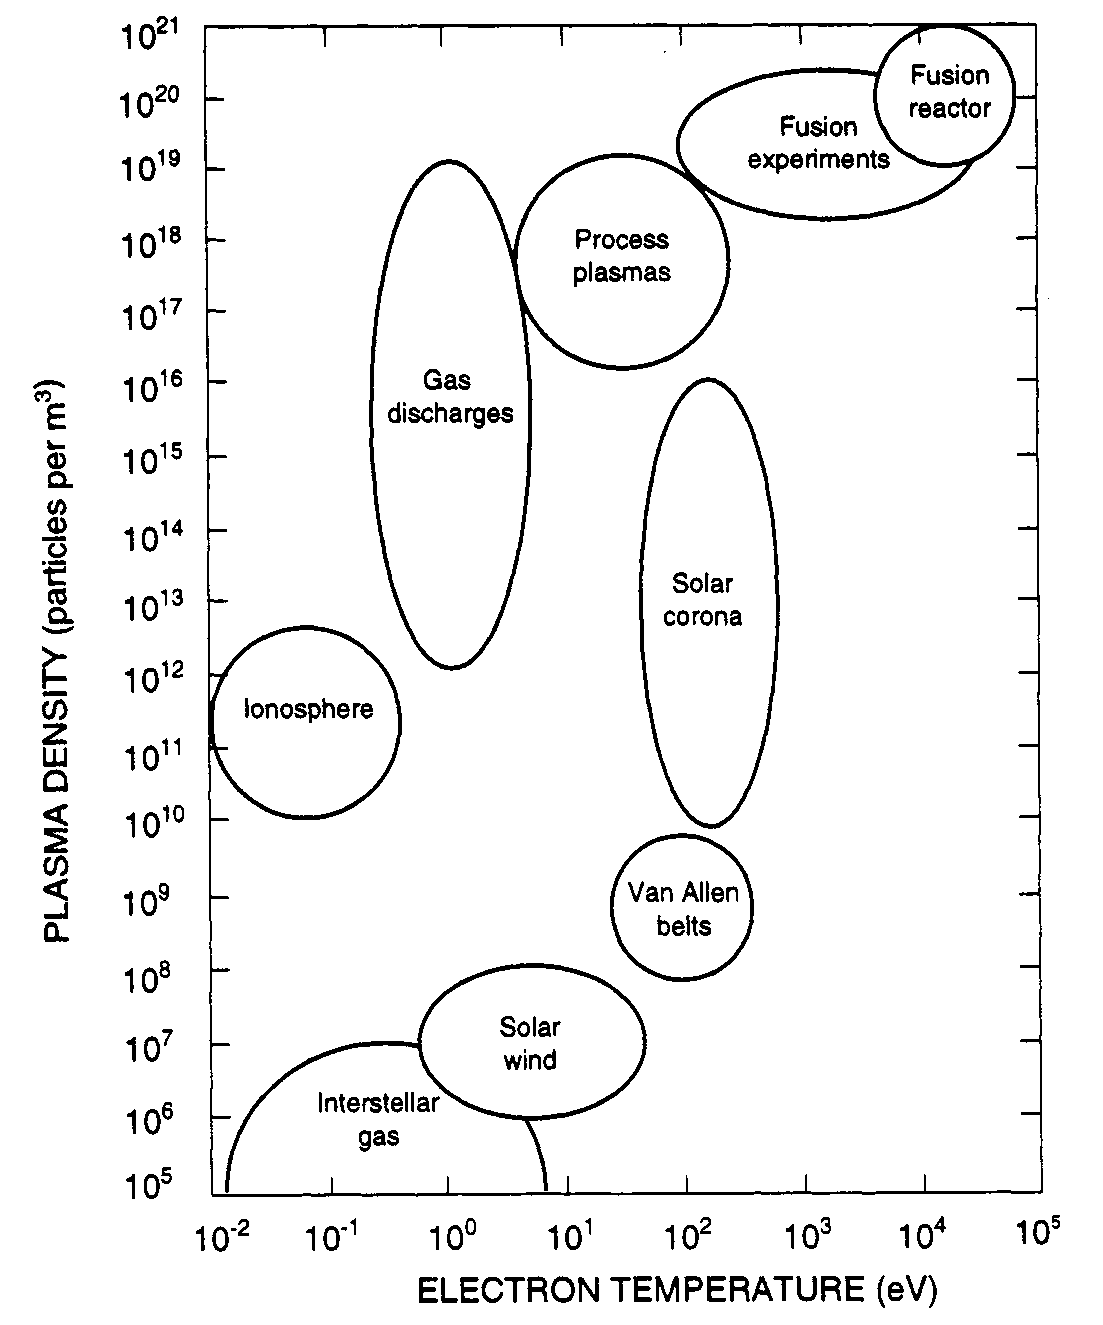
\includegraphics[width = 0.5\textwidth]{figures/theory/plasma_density}
		\end{center}
		\caption{Plasmas occurs both in the hot and dense condiotions in necessary for fusion, as
		well as in the cold and sparse interstellar environment. [NOTE MAKE BETTER FIGURE]
		}
	\end{figure}



    \subsection{Plasma Parameters}
		\label{sec:parameters}
		\subsubsection{Temperature}
		A modern view of temperature comes from kinetic theory developed by
		Maxwell and Boltzmann \citep{swendsen_statistical_2006}. We will not go through it
		here but a treatment is available in \citet{goldston_introduction_1995}.
		Temperature is then related to the average kinetic energy of a particle.
		For an ideal monoatomic gas the kinetic energy is then

		\begin{equation}
			\bar{E}_k = \frac{1}{2} m v_{th}^2 = \frac{3}{2} kT \label{eq:temperature}
		\end{equation}

		Here we have introduced \(v_{th} \equiv  \sqrt{kT/m}\) as the thermal velocity, i.e.
		the average velocity of a particle. It should be mentioned that the fraction in
		front of the temperature is dependent on the degrees of freedom of the particle.
		A monoatomic particle can only move in three directions, but a diatomic particle
		can also vibrate and spin. (Correct?)

		In high energy plasma physics it is also costumary to drop the Boltzmann factor, \(k\),
		in \cref{eq:temperature}, and express temperature directly in electronVolt, \(eV\).
		Electronvolt is defined as the energy it takes to move an elementary charge through
		a potential difference of a \(1\) \si{\volt}, and corresponds to approximately
		\(11600 \si{\kelvin}\). For the space and athmospheric plasmas we are mostly
		dealing with here the temperatures are generally low, so we will use the Kelvin scale
		for temperature.

		If the particles in a plasma collide often compared to the characteristic timescales
		of energy and particle changes, the particle velocity distribution can be approximated
		by a maxwellian distribution. It is only then that the concept of
		temperature is valid \citep{goldston_introduction_1995}.

		\subsubsection{Electron Plasma Frequency}
		The most important timescale in plasma physics is the plasma frequency,

		\begin{equation}
			\omega_{pe} \equiv \sqrt{\frac{ne^2}{\epsilon_0 m_e}}
		\end{equation}

		which corresponds to a typical electrostatic oscillatory frequency.
		Consider an electrically neutral 1D slab, which is then disturbed, from its
		neutrality, by an infinitesimal charge density on one side.

		\begin{equation}
			\sigma = en\delta x
		\end{equation}

		It will have an equal and opposite charge density on the other side. The slab
		will then have an electric field due to the charge density, caused by Gauss' Law.

		\begin{equation}
			\pdv{E_x}{x} = -\frac{\sigma}{\epsilon_0} \qquad\rightarrow\qquad
			E_x = \frac{-en\delta x}{\epsilon_0}
		\end{equation}

		Inserting this field as the only force in Newtons law for a single particle yields

		\begin{equation}
			m\pdv{\delta x}{t} = eE_x = -m\omega_{pe}^2\delta x
		\end{equation}

		The particle will then oscillate around its equilibrium position with
		the electron plasma frequency. The same phenomen often happens in plasma as
		it tries to go back to its equilibrium and is called plasma oscillations,
		or Langmuir oscillations, see \cref{sec:langmuir} for a treatment of plasma oscillations.

		An otherwise useful timescale is the reciprocal of the plasma frequency,
		the plasma period

		\begin{equation}
			\tau_p \equiv 2\pi/\omega_{pe}
		\end{equation}

		Some researchers prefer to define the \(\tau_p\), without the \(2\pi\) prefactor,
		as that makes some consepts neater.

		\subsubsection{Debye Shielding}
		Debye shielding length is the distance at which the electric influence
		from a particle is shielded out by the surrounding plasma.
		Consider a charged particle immersed in a plasma bath. The plasma is in
		a thermodynamically equilibrium, i.e. there is no significant temperature
		gradients. We artificially place a positively charged ion into the plasma.
		This ion will then attract electrons and repel positive ions. There will be a tendency
		for there to be more negativily charged particles, and less positive, near the
		ion, which in effect will work as an electric shield around the ion. The
		distance away from a particle where its field, is typically cancelled out is called the
		Debye Shielding Length, \(\lambda_D\).


		\begin{equation}
			\lambda_D \equiv \sqrt{\frac{\epsilon_0 kT_e}{n_e e^2}}
		\end{equation}

		This is a definition that is often used, \citep{goldston_introduction_1995},
		neglecting the ion influence since they often have a much lower temperature.
		In cases where we also need to account for ions, a more complete definition can be used

		\begin{equation}
			\lambda_D \equiv \sqrt{\frac{\epsilon_0 k T_e}{n_e e^2(1+Z \frac{T_e}{T_i})}}
		\end{equation}

		Due to the earlier argument, and the statistical approach used when deriving it \citep{goldston_introduction_1995},
		there must be a significant amount particles close to the ion to shield it out.

		It should be noted that the shielding length is related \citep{fitzpatrick_plasma_2014} to the
		the plasma period and the thermal velocity through

		\begin{equation}
			\lambda_D \propto \tau_p v_{th}
		\end{equation}


		\subsubsection{Quasineutrality}
		The assumption of quasi-neutrality is often a valid approximation in plasma
		physics. By quasi-neutrality we assume that we in the analysis set the electron
		density equal to the electron density, \(n_e \approx n_i\). This is often called the
		\textit{"plasma approximation"}, see \citep{chen_introduction_1984}. This approximation is often valid on scales
		much larger than the shielding length due to the following arguement. If a
		large volume of plasma lost a significant amount of charge a large electric
		field accompany the density imbalance. This electric field would quickly correct
		the imbalance.

		\subsubsection{Plasma Classification}
        For a plasma description to be useful the system we consider must have
        a typical length scale, \(L\), and time scale, \(\tau\), larger than the Debye length and plasma
        period respectively.

        \[\frac{\lambda_D}{L} \ll 1  \qquad{} \qquad \frac{\tau_p}{\tau} \ll 1 \]


















%Stay here fucker

    %!TEX root=../../thesis.tex

\section{Single Particle Motion}
	To better understand the collective motion of plasma it is useful to consider
	the motions of the single particles that the plasma consists of. By at first
	treating only one particle we can ignore the electromagnetic influence from
	the other particles which greatly simplifies the situation. The Lorentz
	force, \cref{eq:lorentz}, governs the dynamics of a charged particle in a plasma,
	provided that other forces, e.g. gravity, are neglible.
	The Lorentz force consist of a combination of the velocity, \(\vb{v}\), electric field, \(\vb{E}\), and
	magnetic field \(\vb{B}\).
 	\begin{align}
		\vb{F} = q\left(\vb{E} + \vb{v}\cross\vb{B}\right) \label{eq:lorentz}
	\end{align}
	To simplify matters we will only consider particles in static electromagnetic field,
	as that is often a valid approximation on the time and spatial scales of interest.

	\subsection{Gyration}
		\label{sec:gyration}
		Let us consider a situation with a single particle in a static and isotropic external
 		magnetic field, with an initial velocity, as in \citet{goldston_introduction_1995}.
		Newtons Second law together with \cref{eq:lorentz} then gives

		\begin{align}
			m\pdv{\vb{v}}{t} &= q\vb{v}\cross\vb{B} \label{eq:simple_gyration}
			\intertext{The velocity component parallel to the magnetic field is unaffected by the field and
			will remain constant. If we take perform a temporal differention on the
			perpendicular part we get}
			% So we will
			% seperate the velocity into a parallel and perpendicular velocity with respect to the magnetic field,
			% \(\vb{v}=\vb{v}_\parallel + \vb{v}_\perp\). The parallel motion is fully described by
			% \(\pdv{\vb{v}_\parallel}{t} = 0\).
			% We remove the parallel part and perform temporal derivative on the equation of motion to get }
			\pdv[2]{\vb{v}_\perp}{t} &= \frac{q}{m} \pdv{\vb{v}_\perp}{t}\cross \vb{B}
			\intertext{Then we insert \cref{eq:simple_gyration} into the equation and use the vector relation
			\( a\cross b\cross c = b(a\cdot b) - c(a\cdot b) \).}
			\pdv[2]{\vb{\omega}_\perp}{t} + \left(\frac{qB}{m}\right)^2\vb{\omega}_\perp &= 0
		\end{align}

		\begin{figure}
			\centering
			\begin{subfigure}{0.45\textwidth}
				\begin{tikzpicture}
      \draw[->] (0,0) -- (5,0) node[below] {$x$};
      \draw[->] (0,0) -- (0,5) node[left] {$y$};
      \draw (5,5)   node {$\vec{B}$};
      \draw[scale=0.5,domain=0:5,smooth,variable =\x, blue] plot ({\x},{sqrt(\x)});
    %   \draw[scale=0.5,domain=-3:3,smooth,variable=y,red]  plot ({\y*\y},{y});
    \draw[color=blue] plot[id=sin] function{cos(x)}
            node[right] {$f(x) = \sin x$};
\end{tikzpicture}

				\caption{The blue line shows the motion of a particle moving in the presense of a magnetic
				field pointing out of the paper. The particles trajectory is a gyration around the magnetic field lines.}
			\end{subfigure}
			\begin{subfigure}{0.45\textwidth}
				\missingfigure[figwidth=\textwidth]{Gyration E\_parallel}
				\caption{Here we can see a particle experiencing the E-cross-B drift. The motion consists of a gyration
				as well a constant drift along the \(x\)-axis.}
			\end{subfigure}
		\end{figure}


		This differential equation corresponds to a gyration around the magnetic field lines
		with the gyration frequency, \(\omega_c = \frac{qB}{m}\), as the frequency.
		In the last equation we also changed the term describing the rotational motion
		to \(\vb{\omega}_\perp\), which is often used in plasma literature to
		signify gyration.

	\subsection{E-cross-B Drift}
	The E-cross-B drift happens when a particle is moving within static and isotrop
	electric and magnetic fields. The equation of motion, neglecting all forces
	except the electromagnetic, is then

	\begin{align}
		m\pdv{v}{t} &= q(\vb{E} + \vb{v}\cross\vb{B}) \label{eq:EcrossB}
	\end{align}

	As in the previous section we decompose the velocity into a parallel and perpendicular
 	velocity. We also assume there exists a constant drift \(\vb{v}_D\), somewhat unfounded at this stage,
	so that we can seperate the perpendicular motion into the drift and the gyration.
	The velocity is then given by \(\va{v} = \va{v}_\parallel + \va{\omega}_\perp + \va{v}_D\),
	and we insert this into the equation of motion.

	\begin{align}
		m\pdv{}{t}\left( \va{v}_\parallel + \va{\omega}_\perp + \va{v}_D\right) &=
		q \left( \va{E} +   \left( \va{v}_\parallel + \va{\omega}_\perp +
		\va{v}_D \right)  \cross \va{B}_0 \right)
	\end{align}


	As before the parallel velocity is unaffected by the magnetic field we subtract
	it from the equation. From \cref{sec:gyration} we know that the gyration
	part is given by

	\begin{align}
		m\pdv{\vb{\omega}_\perp}{t} &= q\vb{\vb{\omega}_\perp}\cross\vb{B}
	\end{align}

	After we have subtracted these two parts we are left with

	\begin{align}
		\pdv{\va{v}_D}{t} &= \frac{q}{m} \left( \va{E}_\perp + \va{v}_D \cross \va{B} \right)
	\end{align}

	Then we use the previous assumption that the drift velocity is constant,
	cross the equation with \(\vb{B}\) and perform some algebra, see \citet{goldston_introduction_1995} to arrive at

	\begin{align}
		\vb{v}_D &= \frac{\vb{E}\cross\vb{B}}{B^2}
	\end{align}

	As we can see the E-cross-B drift is independent of particle charge and mass,
	which means both the ions and electrons will be drifting at the same velocity
	subject to the drift which will be perpendicular to electric and magnetic fields.

	There several other types of drift, and motions, that appear in various configurations,
	that we will not go through here, i.e. gradient-B drift, curvature drift, polarization drift and magnetic mirror
	to mention a few.

    \section{Kinetic Theory}
    Here we will shortly introduce kinetic theory in relation to plasma physics.
	To consider a large amount of particles we consider a charge and current density
	instead of the individual particles.
	Let \(\mathcal{F}_s\) be the exact phase-space density of a particle species,
	it contains all the positions, velocities for all the particles at
	all times. By integrating over all velocities and multiplying with the charge
	for all species we obtain the charge density, \(\rho_c\).

	\[\rho_c = \sum_s e_s \int \mathcal{F}_s(\vb{r},\vb{v},t)\dd[3]{\vb{v}}\]

	Likewise we find the current density, \(\vb{j}\) by:

	\[\vb{j} = \sum_s e_s \int \vb{v}\mathcal{F}_s(\vb{r},\vb{v},t)\dd[3]{\vb{v}}\]

	Then its seems we can derive all plasma interaction from considering
	the conservation of the phase-space density, coupled with Maxwells equations.
	The phase-space conservation is given by what is known as Vlasovs equation \cref{eq:vlasov}
	\citep{pecseli_waves_2012}).

	\begin{align}
		\pdv{\mathcal{F}}{t} + \vb{v}\cdot\nabla\mathcal{F}_s + \frac{e_s}{m_s}\left( \vb{E} + v\cross\vb{B} \right) \cdot \nabla_v\mathcal{F}_s = 0 \label{eq:vlasov}
	\end{align}

	where \(\nabla_v\) is the velocity grad-operator.
	Unfortunately this expression, combined with Maxwells equations, is only solvable
	for special simple geometries.

    \section{Fluid Description}
	This section aims to provide an overview of the derivation of the fluid equations
	from a Kinetic Theory perspective. First the Vlasov equation is introduced,
	then it is explained how the fluid equations can be obtained by taking different
	order moments of the Vlasov equation. This can help understand the limitations
	of the fluid model of plasma. Lastly a few different approximations
	to make the fluid equations closable.

\subsection{Velocity Moments}
	To investigate plasma as a fluid we have to make certain fluid approximations.
	The plasma is then characterized by local parameters describing particle
	density, kinetic temperature, flow velocity and so on. These parameters refer
	to a small volume of plasma, in contrast with the discussions earlier \cref{sec:single_particle}.
	The time evolution is then governed by the fluid equation, but unfortunately the resulting
	equations are generally less tractable than the usual hydrodynamical
	equations.

	The usual quantity known as the momemt is given by mass times velocity,
	here we will introduce a more general form of moment where the usual moment
	is the first order moment. This will help understand how the fluid
	equations result from averaging over different moments of the general
	transport equation. The zeroth, first and second order moment is respectively
	given by

	\begin{subequations}
		\begin{equation}
			\Phi^0(\vb{v}) = m
		\end{equation}
		\begin{equation}
			\Phi^1(\vb{v}) = m\vb{v}
		\end{equation}
		\begin{equation}
			\Phi^2(\vb{v}) = m\vb{v}\vb{v}
		\end{equation}
	\end{subequations}

	By integrating the moment functions and the distribution function
	\(\mathcal{F}\), over the velocity space we can retrieve different quantities.

	Integrating the zeroth order moment gives the density, if we divide by the
	mass.

	\begin{equation}
			n = \frac{1}{m}\int m \mathcal{F} \dd\vb{v}
	\end{equation}

	Integrating over the first order moment gives the momentum, if we divide
	by density.

	\begin{equation}
			m\vb{v} = \int m \vb{v} \mathcal{F} \dd\vb{v}
	\end{equation}

	We can in fact find the mean of any order moment by integrating the
	distribution function over \(\mathcal{F}\).

	\begin{equation}
		\left< \Phi^n(\vb{v}) \right> = \frac{1}{n} \int \Phi^n \mathcal{F} \dd\vb{v}
	\end{equation}

\subsection{Transport Equation}
	By multiplying the a momentum function, \( \Phi \), with the Vlasov equation, \cref{eq:vlasov},
	we obtain the general momentum transport equation \citep{shu_physics_2010}.

	\begin{equation}
		\pdv{n\left< \Phi^n(\vb{v}) \right>}{t} + \nabla \cdot \left( \left< \Phi^n(\vb{v})\vb{v} \right> \right)
		= \frac{n}{m} \left< \vb{F}_L \cdot \nabla_v \Phi^n(\vb{v}) \right>
	\end{equation}

	This then becomes a conservation equation for the average macroscopic quantity
	\(\left< \Phi \right>\). By using this equation and inserting in the zeroth, first and second order
	moment we obtain the fluid equations, \cref{eq:continuity,eq:momentum,eq:pressure}.
	We refer you to \citet{fitzpatrick_plasma_2014} to see a derivation of the fluid
	equations.


	% To simplify matters we can average over an ensemble to obtain the
	% average distribution function \(\mathcal{\bar{F}}_s\),
	% \[\mathcal{\bar{F}}_s \equiv \left< \mathcal{F}_s\right>_{ensemble}\].
	%
	% The averaged distribution is then used in \cref{eq:vlasov} to make it more tractable.
	% The electric, \(\vb{E}\), and magnetic fields, \(\vb{B}\), is statistically
	% dependent of the distribution function and this leads to correlations when
	% using the averaged distribution. We will not go into those here, so see
	% \textit{\citetitle{fitzpatrick_plasma_2014}}\citep{fitzpatrick_plasma_2014}
	% for a treatment of it.


\subsection{Fluid Equations}
	\label{sec:fluid}
	The generalized fluid equations is given in \cref{eq:continuity,eq:momentum,eq:pressure}, where the three equations
	describe the conservation of mass, momentum and energy respectively. The collision term is negleted.
	We refer you to the earlier mentioned \citet{fitzpatrick_plasma_2014}, although some
	notation differ, for the rather involved derivation to obtain them.

	\begin{subequations}
		\begin{equation}
			\left( \pdv{t} + \vb{u}_s\cdot\nabla \right)n_s + n_s\nabla\cdot \vb{u}_s =0
			\label{eq:continuity}
		\end{equation}
		\begin{equation}
			m_sn_s\left( \pdv{t} + \vb{u}_s \cdot \nabla \right)\vb{u}_s = - \nabla p_s - \nabla \cdot \pi  + n_s\vb{f}_s
			\label{eq:momentum}
		\end{equation}
		\begin{equation}
			\left( \pdv{t} + \vb{u_s} \cdot \nabla \right)p_s =
			- \frac{5}{3} p_s\nabla \cdot \vb{u}_s -
			\frac{2}{3}\pi_s : \nabla{\vb{u_s}}
			- \frac{2}{3}\nabla \cdot \vb{q}_s
			\label{eq:pressure}
		\end{equation}
	\end{subequations}

	% (NOTE TO SELF: NEED TO DEFINE PROPERLY ALL TERMS)
	% To simplify matters we can average over an ensemble to obtain the
	% average distribution function \(\mathcal{\bar{F}}_s\),
	% \[\mathcal{\bar{F}}_s \equiv \left< \mathcal{F}_s\right>_{ensemble}\].
	%
	% The averaged distribution is then used in \cref{eq:vlasov} to make it more tractable.
	% The electric, \(\vb{E}\), and magnetic fields, \(\vb{B}\), is statistically
	% dependent of the distribution function and this leads to correlations when
	% using the averaged distribution. We will not go into those here, so see
	% \textit{\citetitle{fitzpatrick_plasma_2014}}\citep{fitzpatrick_plasma_2014}
	% for a treatment of it.

	The first equation, \cref{eq:continuity}, is the continuity equation, it states that the total mass
	in a volume	should be preserved. \(\vb{u}_s\) is the flow velocity and \(n_s\) is the number density, i.e.
	number of particles in a volume. The divergence terms signifies change due to the compressability of the fluid
	and can in many cases be set to \(0\). The total derivative, i.e. \(\left(\pdv{t} + \vb{u}_s\cdot\nabla \right)\) accounts for
	change in density in a volume taking into account substance exiting and entering.
	The momentum equation \cref{eq:momentum} shows that the fluid momentum change, left hand side,
	is due to pressure gradients, \(\nabla p_s\), visceous forces, \(\nabla \cdot \pi \) and external forces, \(n_s\vb{f}_s\),
	per unit volume.
	Lastly we have the energy equation, in its pressure form, which shows that changes to thermal
	energy, \(p = nkT\), is caused by compression, \(p_s\nabla \cdot \vb{u}_s\), visceous effects \(\pi_s : \nabla{\vb{u_s}}\)
	and heat transport	\(\frac{2}{3}\nabla \cdot \vb{q}_s\).
	The fluid equations is in general not closeable and adding higher order moments
	always introduces more unknowns. Due to this one generally uses different closing
	schemes, some of which is described in the next section, to make them tractable.

\subsection{Plasma States}
	Plasma can be classified according to which	approximations and simplifications
	that are valid for them. Here we will go through a few of them.

	\subsubsection{Local Thermodynamic Equilibrium}
	A plasma is said to be in a \textit{local thermodynamic equalibrium} (LTE)
	if the phase-space distribution is locally Maxwellian. This means the variations
	in temperature is slow enough that we can consider it to flow no heat. We can also ignore
	the viscosity due to there being little local variations to the momentum flow.

	\begin{align}
		\mathcal{F}_m = \frac{n}{(2\pi )^{3/2}v_t^3} \exp{-\frac{(v-u)^2}{2v_t^2}}
	\end{align}

	Since the viscosity tensor, \(\vb{\pi}\), and the heat flux tensor, \(\vb{q}\)
	contains odd integrals over the distribution, see \citet{fitzpatrick_plasma_2014},
	they dissappear.

	\subsubsection{Cold Plasma}
	In what we consider a cold plasma the pressure, \(p\), and viscosity, \(\pi\), is set to zero.
	This can be useful if the velocities of interest far exceed the thermal velocities.
	(ADD MORE)


	\subsubsection{Isothermal}
	An isothermal plasma is one where we assume an infinite heat conductivity,
	this means the temperatures is constant in all space and time. This can be used to
	describe macroscopic plasma.
	(ADD MORE)

    \section{Plasma Oscillations}
	\label{sec:langmuir}

	Plasma oscillations, also called Langmuir oscillations, is the basic resulting
	oscillation	that happens as a plasma tries to reach a stable equilibrium, due to
	a small perturbation of its density.
	We will use this to show how the fluid equations can be closed for a simple system
	using assumptions. This is also very suited to test simulations, as we do later
	in \cref{sec:langmuir_verification}.

	Here we will consider an one specie plasma fluid consisting of electrons under local thermal equilibrium, LTE.
	The electron density, \(n_0\) and pressure, \(p_0\), is initally homogenous.
 	The fluid has a vanishing flow, \(\va{u}_0 = 0\), and no initial potential gradient \(\phi_0 = 0\).
	The ele
 	See \citet{pecseli_waves_2012} for a another discussion.

	A small perturbation of the electron density will cause the electric field
	to try to restore the equilibrium. When the electrons reach the equilibrium
	position they will have a kinetic energy and will overshoot.This will cause
	a new perturbation away from the equilibrium.

	Under the LTE conditions the fluid equations simplify to

	\begin{subequations}
		\begin{equation}
		\pdv{n_e}{t} + \nabla \cdot (n_e \va{u}_e) = 0
		\end{equation}
		\begin{equation}
		m_en_e\left( \pdv{}{t} + \va{u}_e \cdot \nabla \right)\va{u}_e = e n_e \nabla \phi - \nabla p_e
		\end{equation}
		\begin{equation}
		\left( \pdv{}{t} + \va{u}_e \cdot \nabla \right) p_e + \frac{5}{3} p_e\nabla \cdot \va{u}_e = 0
		\end{equation}
	\end{subequations}
	Since this set of equations have more unknowns than equations so we need additional information
	to close the set. Here we can use the Poisson equation to close it.
	\begin{equation}
	\epsilon_0 \nabla^2 \phi = e\left( n_e - n_0 \right)
	\end{equation}

	Now we let a small perturbation, denoted by a tilde, happen to the equilibrium.
	Since we are free to choose an inertial reference frame, we select one co-moving
	with the plasma so the inital fluid velocity is \(\va{u}_0=0\). We also select
	the reference potential so the initial potential, \(\phi_0\),  is \(0\).


	\begin{equation*}
	\text{Perturbation} \rightarrow
	\begin{cases}
	  n_e = n_0 + \tilde{n}_e\\
	  p_e = p_0 + \tilde{p}_e\\
	  \va{u}_e = \tilde{\va{u}}_e\\
	  \phi = \tilde {\phi}
	\end{cases}
	\end{equation*}

	Since the pertubation is small, we can say that any part that contains
	second order terms of perturbation of a quantity will be much smaller than the value
	of the quantity, \(q \gg\tilde q \tilde q\). So even though we may miss some processes
	by doing this, we can drop the second order perturbation terms.
	This process is called linearization.

	Inserting the perturbation and linearizing the equations we get:

	\begin{subequations}
	  \begin{equation}
	    \pdv{\tilde{n}_e}{t} + \nabla \cdot (n_0 \tilde{\va{u}}_e) = 0 \label{eq:langmuir_continuity}
	  \end{equation}
	  \begin{equation}
	    m_e \pdv{\tilde{\va{u}}_e}{t}  = e  \nabla \tilde{ \phi} - \frac{\nabla \tilde{p}_e}{n_0}
	  \end{equation}
	  \begin{equation}
	     \pdv{\tilde{p}}{t} +\frac{5}{3}p_0 \nabla \cdot \tilde{\va{u}}_e = 0 \label{eq:langmuir_energy}
	  \end{equation}
	  \begin{equation}
	    \epsilon_0 \nabla^2 \tilde{\phi} = e\tilde{n}_e
	  \end{equation}
	\end{subequations}

	Then we combine the continuity and energy equations, \cref{eq:langmuir_continuity} and \cref{eq:langmuir_energy}.

	\begin{align}
	\pdv{}{t}\left( \frac{\tilde{p}_e}{p_0} + \frac{5}{3} \frac{\tilde{n}_e}{n_0} \right) &= 0
	\end{align}

	The perturbed pressure and density are proportional, \(\nabla \tilde{p}_e = \left(5p_0/3n_0\right)\nabla \tilde{n}_e\).
	Assuming plane wave solutions along the x-axis, the differential operators become \(\nabla \rightarrow ik\)
 	and \(\pdv{}{t} \rightarrow -i\omega\), we can solve for the dispersion relation.

	\begin{align}
	\epsilon(\omega, k) = 1 + \frac{5}{3} \lambda_{se}^2k ^2 -  \frac{\omega^2}{\omega_{pe}^2}
	\end{align}

	Here the electron debye length, \(\lambda_{D}\), and the plasma frequency, \(\omega_{pe}\), have been inserted.

% \section{Langmuir Oscillations}
% 	REDO, You have already done this in a neater way before!!!!!!!!!!!!
%
% 	In a we consider a homogenous and isotropic plasma, in stable equilibrium,
% 	and let the electrons be pushed, causing a slight perturbation of the equilibrium.
% 	The slightly uneven distribution will cause an electric field pushing against
% 	the perturbation and try to restore the equilibrium. When the electrons reach
% 	the equilibrium position they have a kinetic energy and will overshoot
%  	causing an equal opposite perturbation. Then it repeats and we have a simple
% 	oscillation of the electron density.
%
% 	Certain assumptions are necessary to derive the oscillation mathematically.
% 	First the plasma needs to be in a homogenous and isotropic equilibrium state
%  	so the spatial and temporal derivatives is zero. The magnetic field strength
% 	also needs to be small enough to be safely ignored.	We then consider movements
% 	on a timescale so that the inertial effects of the electrons are important,
% 	while the ions are considered stationary.
%
% 	We start from the electron fluid motion equation,
% 	\begin{equation}
% 	mn_e \left( \pdv{}{t} + \vec{u} \cdot \nabla \right)\vec{u} = -en_e\vec{E} - \nabla p_e
% 	\end{equation}
% 	and we consider a small perturbation to the equilibrium state so the quantities becomes:
% 	\begin{equation}
% 	\vec{u} \approx \vec{u}_0 + \vec{\tilde{u}}; \qquad{}
% 	\vec{E} \approx \tilde{\vec{E}}; \qquad{}
% 	n \approx n_0 + \tilde{n};\qquad{}
% 	p \approx p_0 + \tilde {p}
% 	\end{equation}
% 	Here the subscript for the electron is dropped, the subscript \(0\) is
%  	the equilibrium state and the tilde is the perturbation. Then we apply
% 	linearization to the equation, so that all the second order terms of the
% 	perturbation goes away.
% 	\begin{equation}
% 	mn_0\pdv{}{t} \tilde{\vec{u}} = -en_0\vec{\tilde{E}} - \nabla \tilde{p_e}
% 	\end{equation}
% 	For simplicities sake the perturbation is a plane wave in the x-direction, \(exp[i(kx - i\omega)]\),
% 	as well as what we will program for verification use. Then the differential
% 	operators become \(\nabla \rightarrow ik\) and \(\pdv{}{t} \rightarrow -i\omega\),
% 	using the relation \(\tilde{p} = {3T\tilde{n}}\), see cite{Goldston INtro to plasma 1995}.
% 	Then the x-component of the electron motion equation becomes:
% 	\begin{equation}
% 	i\omega mn_0 \tilde{u} = e n_0 \tilde{E} + i 3 kt\tilde{n}
% 	\end{equation}
%
% 	Using the same procedure the electron continuity equation,
% 	\(\pdv{n}{t} + \nabla \cdot (\vec{u} n) = 0 \), becomes
% 	\begin{equation}
% 		-i\omega \tilde{n} = ikn_0 \tilde{u}
% 	\end{equation}
%
% 	Next we look poisson's equation, \(\epsilon_0 \nabla \cdot \vec{E} = e(n_i-n_e) \), which using the same procedures,
% 	as well as letting the ion density cancel the equilibrium electron density,	ends up as
% 	\begin{equation}
% 		ik\epsilon_0\tilde{E} = -\tilde{n}
% 	\end{equation}

    \section{Magnetohydrodynamics}
    \label{sec:MHD}
    In a plasma there are usually several types of species, then it follows that
    each specie needs its own set of fluid equations. Magnetohydrodynamics, (MDH),
    is an attempt to simplify this situation by combining it into one electrically
    conducting fluid. Conventional MHD assumes local thermodynamical equilibrium,
    negligable electron inertia and quasi-neutrality \citep{goldston_introduction_1995}.
    This simplifies Maxwell's equations to

    \begin{subequations}
		\begin{equation}
			\nabla \cross \vb{B} = \mu_0 \vb{j}
		\end{equation}
		\begin{equation}
			\nabla \cross \vb{E} = -\pdv{\vb{B}}{t}  \label{eq:mhd_eCurl}
		\end{equation}
		\begin{equation}
			\nabla \cdot \vb{B} = \nabla \cdot \vb{E} = 0
		\end{equation}
	\end{subequations}
%
    The MHD fluid can be considered a neutral fluid with a current running through it
    \citep{hockney_computer_1988}. The current is described by the conductivity \(\sigma\)
    and the bulk velocity \(\vb{v}\) and is given as

    \begin{equation}
        \vb{j} = \sigma \vb{v}
    \end{equation}
%
    With the condition that the condictivity is high and a finite current \cref{eq:mhd_eCurl}
    becomes

    \begin{equation}
        \pdv{\vb{B}}{t} = \nabla \cross \left( \vb{v} \cross \vb{B} \right)
    \end{equation}
%
    Then it remains to close the MHD equations by continuity and momentum conservation,
    where \(\rho\) is the mass density and \(p\) is the scalar pressure.

    \begin{subequations}
		\begin{equation}
			\pdv{\rho}{t} = \nabla \cdot (\rho \vb{v})
		\end{equation}
		\begin{equation}
            \rho \pdv{\vb{v}}{t} = - \nabla p + \vb{j} \cross \vb{B}
		\end{equation}
	\end{subequations}
%

    \section{Numerical Simulations}

	The mathematical description of plasma is helpful to improve our
	understanding of the physics, many problems doesn't fall neatly into convenient
	assumptions or are untractable. Then we need to turn to experiments and computer simulations
	solve them. All of these methods work in symbiosis and is interdependent
	on each other. Numerical simulations bears many similarities to
	experiments, but it also has the advantage of being applied to situations that no
	experiment can reproduce. In addition physical experiments often has constraints on what can
 	be measured directly, while numerical experiments have all the wanted data readily available.
	Modelling generally needs to be validated against
	against experiments and has a foundation built upon theory. As the computational
	resources have improved, more sophisticated simulations have been possible.
	Plasma simulations vary from fluid descriptions, as MHD codes, to kinetic descriptions,
	as Particle-in-Cell and Vlasov codes, with hybrid codes inbetween as well.
	This thesis focuses on the development of a Particle-in-Cell code, but here we will give a brief
	overview of other modelling approaches as well.
	%
	% As there are several theoretical branches within the field of plasma physics,
	% magnetohydrodynamics, kinetic theory (Note to self:  Need better overview, and citations),
	% that are suited to investigate plasma physics at different scales and different phenonema,
	% there are also different approaches to conduct numerical plasma studies.
	% Plasma simulation codes can be classified along the extent they are using a
	% kinetic kinetic or fluid description of the plasma. Kinetic codes include
	% Vlasov simulations (cite), Fokker-Planck simulations (Cite) and particle codes like the
	% Particle-in-Cell code, that the development of, was a large part of this master thesis.
	% Plasma fluid simulations are called MHD and are based on magnetohydrodynamical theory, (mention some).
	% In the fluid description some of the detailed physics is averaged out and this causes
	% MHD codes to be unsuited to study results depending on some small scale phenomena.
	% Their advantage is that due to the reduced detail they can simulate on a much larger scale.
	% Kinetic simulations generally have more detail and capture more physics (rewrite),
	% and as a tradeof they are restricted to simulate over a physical domain due to
	% limited computation power and memory storage.
	% Since the relevant timescales vary vastly between ions and electrons a multitude
	% of hybrid codes has also been developed. (Search for multitude of hybrid codes and ref).
	% These types of codes can e.g. treat some of the species as fluids and some as
	% particles capturing the wanted phenomena. Particle based codes can also be combined
	% with molecular dynamics code, if the algorithm is unsuited in a regime.

	\subsubsection{MHD}
		Magnetohydrodynamical codes solve the one-fluid equations, given in \cref{sec:MHD},
		with various approaches and has
		similarities to Computational Fluid Dynamics. For the fluid equations
		to be a reasonable description of plasma, the dynamics needs to happen at much larger scales
		than the Debye Shielding Length. This approach has been widely used in large scale
		plasma simulations such as astrophysics, see \citet{hawley_numerical_1995} where an MHD approach is discussed with regards to astrophysical problems,
 		and space physics, see \citet{watanabe_global_1990} for an investigation of the solar wind-magnetsphere interaction.

	\subsubsection{Particle-in-Cell}
		Particle-in-Cell models the particles directly, this has the advantage that
		few approximations are done, but computational increases fast with more particles.
		Numerical PiC codes has been used extensively to research charging- and wake-effect on spacecraft
		operating in the upper earth atmosphere \citep{}.

	\subsubsection{Vlasov}
		Vlasov codes takes the kinetic description as the starting point and are often used
		in plasma laser modelling \citep{bertrand_nonperiodic_1990}. It has an advantage over
		PiC in low density zones, where there is often too few particles for PiC.

    \section{Collisions: MCC-Null Model}
    First we will go through the Monte Carlo Collisional model and then show how
    the Null-Collision scheme can reduce the amount of arithmetic operations.
    To avoid spending computational time on the neutral particles we consider
    them as background species.
    We assume for simplicity that the neutral particles are
    uniformly distributed, with a normal velocity distribution.

    Particle species \(s\) has \(N\) type of collisions with a target species. Each particle
    has kinetic energy

    \begin{equation}
        \varepsilon_i = \frac{1}{2}m_s \left(v_x + v_y +v_z \right)
    \end{equation}
    %
    The collisional cross section \(\sigma_j\) for each type of collision is dependent on the
    kinetic energy of the particle and the total cross section is given by adding
    together all the types of collisions.

    \begin{equation}
        \sigma_T(\varepsilon_i) = \sum_j^N \sigma_j(\varepsilon_i)
    \end{equation}
    %
    The probability that a particle has a collision with a target species, in one timestep, is
    be dependent on the collisional cross section, distance travelled, \(\Delta r_i = v_i\Delta t\), and the
    density of the target specie, \( n_t(\vec{r_i}) \) by the following relation.

    \begin{equation}
        P_i = 1-\exp{-v_i\Delta t \sigma_T(\varepsilon_i) n_t(\vec{r_i} }
    \end{equation}

    In a Monte Carlo model we say that a collision has taken place for a particle if a random number
    \(r = [0,1]\), is smaller than \(P_i\).
    To compute \(P_i\) for each particle, we need to find \(\varepsilon_i\), all the cross sections
    \(\sigma_j\), and the density \(n_t(\vec{r_i}\). This demands many floating point operations for
    each particle, so we will use a Null-Collisional model to only compute the collisional
    probability for a subset of the particles. We compute a maximal collisional frequency
    \begin{equation}
        \nu'= \max({v_i\Delta t \sigma_T(\varepsilon_i)})\max({n_t(n_t)})
    \end{equation}
    %
    and consider if it was a dummy or one of the proper collisions, if \(r\) is smaller
    than the resulting constant \(P_{Null} =  1-\exp{\nu'}\).

    The maximum collisional frequency may need to be recomputed each timestep due
    to the density of the target specie,  \(n_t\), changing. The algorithm for
    each particle is then.
    \\ \\
    \begin{table}
        \begin{algorithmic}
            \For{Each particle}
                \If {$r \leq P_{Null}$}\\
                    \begin{tabular}{r c l l}
                        & \(r\) &\(\leq \nu_0(\varepsilon_i)/\nu' \qquad\)
                        & Type 0
                        \\
                        \(\nu_0(\varepsilon_i)/\nu' \leq\) & \(r\) & \( \leq (\nu_0(\varepsilon_i) + \nu_1(\varepsilon_i))/\nu'\)
                        & Type 1
                        \\
                        & \(\vdots\) &
                        \\
                        \(\sum_j(\nu_j(\varepsilon_i))/\nu' \leq\) & r & & Type Null
                    \end{tabular}
                \EndIf
            \EndFor
        \end{algorithmic}
        \caption{Algorithm to select a particle collisions (Need to be improved)}
    \end{table}

% %
\chapter{Method}
    
\section{Particle-in-Cell}
 To investigate the mechanics involved in a wide variety of plasma phenomenens,
 computer simulation. Particle-in-Cell, PiC, is a model that takes a particle based approach,
 where each particle is simulated seperately, or a collection. If we naively would
 attempt to compute the electrical force between each particle, the necessary
 computational power would grow quickly as the number of particle increases, \(\order{#particles^2}\).
 Since a large number of particles is often neccessary the PiC method seeks to
 the problem by computing the electrical field produces by the particles, and then
 compute the force on the particle directly from the field instead. From the charge
 distribution we can find the electric potential through the use of Poissons
 equation, \cref{eq:poisson}, and subsequently find the electrical field from the electrical potential.
 So an important part of a PiC simulation is an numerically efficient Poisson Solver.

	\begin{align}
		\nabla ^2 \Phi &= -\rho \qquad \text{in} \qquad \Omega \label{eq:poisson}
	\end{align}

	The problem also need boundary conditions in which we will focus on periodic,
	Dirichlet and Neumann boundary conditions.



	\subsection{Spectral Methods}
		The spectral methods is based on Fourier transforms of the problem and solving
		the problem in it's spectral version, see \citep{shen_efficient_1994}, for an
		implementation of an spectral poisson solver. They are efficient solvers that
		can be less intricate to implement (?), but can be inaccurate for complex geometries.

		When looking for a solution with a spectral method we first rewrite the
		functions as Fourier series, which for the three-dimensional Poisson equation would be

		\begin{align}
			\nabla^2 \sum A_{j,k,l} e^{i(jx + ky + lz)} &= \sum B_{j,k,l} e^{i(jx + ky + lz)}
			\intertext{From there we get a relation between the coefficients}
			A_{j,k,l} &= -\frac{B_{j,k,l}}{j^2 + k^2 + l^2}
			\intertext{Then we compute the Fourier transform of the right hand side obtaining
			the coefficients \(B_{j,k,l}\). We compute all the coefficients \(A_{j,k,l}\)
			from the relation between the coefficients. At last we perform a inverse
			Fourier transform of the left hand side obtaining the solution.}
		\end{align}

	\subsection{Finite Element Methods}

		The finite element is a method to numerically solve a partial differential
		equations (PDE) first transforming the problem into a variational problem and
		then constructing a mesh and local trial functions, see \cite{alnaes_fenics_2011}
		for a more complete discussion.

		To transform the PDE to a variational problem we first multiply the PDE by a
		test function \(v\), then it is integrated using integration by parts on the
		second order terms. Then the problem is separated into two parts, the bilinear
		form \(a(u,v)\) containing the unknown solution and the test function and the
		linear form \(L(v)\) containing only the test function.

		\begin{align}
			a(u,v) = L(v)	\qquad v\epsilon \hat{V}
		\end{align}

		Next we construct discrete local function spaces of that we assume contain
		the trialfunctions and testfunctions. The function spaces often consists of
		locally defined functions that are \(0\) except in a close neighbourhood of
		a mesh point, so the resulting matrix to be solved is sparse and can be computed
		quickly. The matrix system is then solved by a suiting linear algebra algorithm,
		before the solution is put together.


\section{Multigrid}
	The multi grid, MG, method used to solve the Poisson equation and obtain the
	electric field is a widely used and highly efficient solver for elliptic equations,
	having a theoretical scaling of \(\order{N}\) \citep{press_numerical_1988},
	where \(N\) is the grid points. Here I will go through the main theory and
	algorithm behind the method, as explained in more detail in \citep{press_numerical_1988,trottenberg_multigrid_2000}
	as well as go through some of possible algorithms to parallelize the method.

	We want to solve a linear elliptic problem,
		\begin{align}
			\mathcal{L} u = f
		\end{align}
	where \(\mathcal{L}\) is a linear operator, \(u\) is the solution and \(f\) is a source term. In our specific case the operator is given by the laplacian, the source term is given by the charge density and we solve for the electric potential.

	We discretize the equation onto a grid of size \(q\).
	\begin{align}
		\mathcal{L}_q u_q &= f_q \label{eq:difference}
	\end{align}

	Let the error, \(v_q\) be the difference between the exact solution and an approximate solution to the difference equation (\ref{eq:difference}), \( v_q = u_q - \tilde{u}_q \). Then we define the residual as what is left after using the approximate solution in the equation.

	\begin{align}
		d_q &= \mathcal{L}_q \tilde{u}_q - f_q
	\end{align}

	Since \(\mathcal{L}\) is a linear operator the error satisfies the following relation

	\begin{align}
		\mathcal{L}_q v_q &= \mathcal{L}(u_q - \tilde{u}_q)  + (f_q- f_q)
		\\
		\mathcal{L}_q v_q &= - d_q \label{eq:diff_MG}
	\end{align}

	In the multigrid methods instead of solving the equation directly here, we set up a system of nested coarser square grids, \(\mathfrak{T}_1 \subset \mathfrak{T}_2 \subset \cdots \subset \mathfrak{T}_\ell\), where \(1\) is the coarsest grid and \(\ell\) is the finest. Then the main thought behind the methods is that instead of solving the problem directly on the initial grid, we use restriction, \( \mathcal{R} \), and interpolation, \( \mathcal{P} \), operators to change the problem between the different grid levels and solve them on there. (Fix previous sentence) Due to the fewer grid points the problem is faster to solver on the coarser grid levels than on the fine grid.

	If we then apply a restriction operator on the residual we go down a level on the grids and the opposite for the interpolation operator.

	\begin{align}
		\mathcal{R} d_q = d_{q-1} \qquad \text{and} \qquad \mathcal{P} d_q = d_{q + 1}
	\end{align}


	\subsection{Algorithm}
		A sequential algorithm for a two grid V shaped algorithm, where the coarse grid and fine grid has respectively \(q = 1,2\).

	\begin{itemize}
		\item Initial approximation. \(\tilde{u}\)
		\item for \(i < \) nCycles:
			\begin{itemize}
				\item Presmooth: \(\hat{u}_2 = S_{pre}(u)_2\)
				\item Calculate defect: \( d_2 = f_2 - \mathcal{L}\hat{u}_2\)
				\item Restrict defect: \( d_1 = Rd_2 \)
				\item Initial guess: 	\( \tilde{u}_1 = 0 \)
				\item Solve (G-S RB): 	\( L_1 \tilde{u}_1 = d_1 \)
				\item Interpolate:		\( \tilde{u}_2 = I \tilde{u}_1 \)
				\item Add correction:	\( u^{new}_2 = \hat{u}_2 + \tilde{u}_2 \)
			\end{itemize}
	\end{itemize}

	\subsection{Smoothing: Gauss-Seidel}
		Relaxation methods, such as Gauss-Seidel, work by looking for the setting up the equation as a diffusion equation, and then solve for the equilibrium solution.

		So suppose we want to solve the elliptic equation
		\begin{align}
			\mathcal{L}u &= \rho
			\intertext{Then we set it up as a diffusion equation}
			\pdv{u}{t} &= \mathcal{L}u - \rho
			\intertext{By starting with an initial guess for what \(u\) could be the equation will relax into the equilibrium solution \(\mathcal{L}u = \rho\).
			By using a Forward-Time-Centered-Space scheme to discretize, along with the largest stable timestep \(\Delta t = \Delta^2 / (2\cdot d))\) (Double check the factor.), we arrive at Jacobi's method, which is an averaging of the neighbors in addition to a contribution from the source term. By using the already updated values for in the calculation of the \(u^{new}\) we arrive at the method called Gauss-Seidel which for two dimensions is the following}
			u^{n+1}_{i,j} &= \frac{1}{4}\left( u^n_{i+1,j} + u^{n +1}_{i-1,j} + u^{n}_{i, j+1} + u^{n+1}_{i,j-1}  \right) - \frac{\Delta^2 \rho_{i,j}}{4}
		\end{align}

		To achieve a vectorization of the calculation of \(u^{n+1}_{i,j}\) we will use Red and Black ordering, first calculating the odd nodes and then the even nodes, so the method has the available information.




\section{Parallelization}
	For the parallelization of an algorithm there is two obvious issues that need to be addressed to ensure that the algorithm retains a high degree of parallelization; communication overhead and load imbalance \citep{hackbusch_multigrid_1982}. Communication overhead means the time the computational nodes spend communicating with each other, if that is longer than the actual time spent computing the speed of the algorithm will suffer, and load imbalance appears if some nodes need to do more work than others causing some nodes to stand idle.

	Here we will focus on multigrid of a 3D cubic (to be expanded to rectangular cubes) grid, where each grid level has half the number of grid points. We will use grid partitioning to divide the domain, GS-RB (Gauss-Seidel Red-Black) as both a smoother and a coarse grid solver.

	We need to investigate how the different steps: interpolation, restriction, smoothing and the coarse grid solver, in a MG method will handle parallelization.

	\subsection{Grid Partition}
		\label{sec:grid_partitioning}
		There are several well explored options for how a multigrid method can be parallized, for example Domain Decomposition \citep{arraras_domain_2015}, Algebraic Multigrid \citep{stuben_review_2001}, see \citet{chow_survey_2006} for a survey of different techniques. Here we will focus on Geometric Multigrid (GMG) with grid partitioning used for the parallelization, as described in the books \cite{trottenberg_multigrid_2000, hackbusch_multigrid_1982}.

		With grid partitioning we divide the grid \(\mathcal{T}\) into geometric subgrids, then we can let each processes handle one subgrid each, as we will see it can be useful when using the G-S RB smoothing to let the subgrids overlap 1 layer deep. since it on the edges of the subgrid it will need the adjacent node values.

	\subsection{Distributed and accumulated data}
		During the parallel execution of the code there can be useful to keep track of the different data structures and what needs to be accumulated over all the computational nodes and what only needs to be distributed on the individual computational nodes.

		\begin{itemize}
			\item \(u\) solution (\(\Phi\))
			\item \(w\) temporary correction
			\item \(d\) defect
			\item \(f\) source term (\(\rho\))
			\item \(\mathcal{L}\) differential operator
			\item \(\mathcal{I}\) interpolation operator
			\item \(\mathcal{R}\) restriction operator
			\item \( \va{u}\) Bold means accumulated vector
			\item \( \tilde{\va{ u }} \) is the temporary smoothed solution
		\end{itemize}

		\begin{itemize}
			\item Accumulated vectors:	\(\va{u}_q\), \( \hat{\va{u}}_q \), \(\tilde{\va{u}}_q\), \(\hat{\va{w}}_q\) \(\va{w}_{q-1}\), \(\va{I}\),\(\va{R}\)
			\item Distributed vectors:  \( f_q \), \(d_q\), \(d_{q-1}\)
		\end{itemize}
		% Algorithm: P is the number of processes
		% \begin{itemize}
		% 	\item If (q == 1): Solve: \(\sum_{s=1}^P\mathcal{L}_{s,1} \va{u}_1 = \sum_{s=1}^Pf_{s,1}\)
		% 	\item else:
		% 		\begin{itemize}
		% 			\item Presmooth: \( \hat{\va{u}}_q = \mathcal{S}_{pre} \va{u_q}\)
		% 			\item Compute defect: \( d_q = f_q - \mathcal{L}_q \hat{\va{u}}_q \)
		% 			\item Restrict defect: \( d_{q -1} = \mathcal{R} d_q \)
		% 			\item Initial guess:   \( \va{w}_{q-1} = 0 \)
		% 			\item Solve defect system: \( \va{w}_{q-1} = PMG(\va{w}_{q-1}, d_{q -1} ) \)
		% 			\item Interpolate correction: \( \va{w}_q = \mathcal{R} \va{w}_{q-1} \)
		% 			\item Add correction:		\( \tilde{\va{u}}_q = \hat{\va{u}}_q + \va{w}_q \)
		% 			\item Post-smooth:			\( \va{u}_q = \mathcal{S}_{post}\)
		% 		\end{itemize}
		% \end{itemize}


	\subsection{Smoothing}
		% Will use G-S with R-B ordering, supposedly good parallel properties \citep{chow_survey_2006}. Follow algorithm I in \cite{adams_distributed_2001} (alternatively try to implement the more complicated version)?

		We have earlier divided the grid into subgrids, with overlap, as described in subsection \ref{sec:grid_partitioning} and given each processor responsibility for a subgrid. Then do a a GS-RB method we start with an approximation of \(u^{n}_{i,j}\). Then we will obtain the next iteration by the following formula

		\begin{align}
			u^{n+1}_{i,j} &= \frac{1}{4}\left( u^n_{i+1,j} + u^{n +1}_{i-1,j} + u^{n}_{i, j+1} + u^{n+1}_{i,j-1}  \right) - \frac{\Delta^2 \rho_{i,j}}{4}
		\end{align}

		We can see that the for the inner subgrid we will have no problems since we have all the surrounding grid points. On the edges we will need the adjacent grid points that are kept in the other processors. To avoid the algorithm from asking neighboring subgrids for adjacent grid points each time it reaches a edge we instead update the entire neighboring column at the start. So we will have a 1-row overlap between the subgrids, that need to be updated for each iteration.


	\subsection{Restriction}
		For the transfer down a grid level, to the coarser grid we will use a half weighting stencil. In two dimensions it will be the following

		\begin{align}
			\mathcal{R} &= \frac{1}{8}
			\begin{bmatrix}
				0 & 1 & 0
				\\
				1 & 4 & 1
				\\
				0 & 1 & 0
			\end{bmatrix}
		\end{align}

		With the overlap of the subgrids we will have the necessary information to perform the restriction without needing communication between the processors \citep{hackbusch_multigrid_1982}.

	\subsection{Interpolation}
		For the interpolation we will use bilinear interpolation:

		\begin{align}
			\mathcal{I} &= \frac{1}{4}
			\begin{bmatrix}
				1 & 2 & 1
				\\
				2 & 4 & 2
				\\
				1 & 2 & 1
			\end{bmatrix}
		\end{align}

		Since the interpolation is always done after GS-RB iterations the the outer part overlapped part of the grid updated, and we can have all the necessary information.

	\subsection{Scaling}
		\subsubsection{Volume-Boundary effect}
		While a sequential MG algorithm has a theoretical scaling of \(\order{N}\) \citep{press_numerical_1988}, where \(N\) is the number of grid points, an implementation will have a lower scaling efficiency due to interprocessor communication. We want a parallel algorithm that attains a high speedup with more added processors \(P\),  compared to sequential \(1\) processor algorithm. Let \(T(P)\) be the computational time needed for solving the problem on \(P\) processors. Then we define the speedup \(S(P)\) and the parallel efficiency \(E(P)\) as

		\begin{align}
			S(P) = \frac{T(1)}{T(P)} \qquad E(P) = \frac{S(P)}{P}
		\end{align}

		A perfect parallel algorithm would the computational time would scale inversely with the number of processors, \(T(P) \propto 1/P\) leading to \( E(P) =1 \). Due to the necessary interprocessor communication that is generally not achievable. The computational time of the algorithm is also important, if the algorithm is very slow but has good parallel efficiency it is often worse than a fast algorithm with a worse parallel efficiency.

		The parallel efficiency of an algorithm is governed by the ratio between the time of communication and computation, \(T_{comm}/T_{comp}\). If there is no need for communication, like on \(1\) processor, the algorithm is perfectly parallel efficient. In our case the whole grid is diveded into several subgrids, which is assigned to different processors. In many cases the time used for computation is roughly scaling with the interior grid points, while the communication time is scaling with the boundaries of the subgrids. If a local solution method is used on a local problem it is only the grid points at the boundary that needs the information from grid points on the other processors. Since the edges has lower dimensionality than the inner grid points. So when the problem is is increasing the time for computation grows faster than the time for communication, and a parallel algorithm often has a higher parallel efficiency on a larger problem. This is called the Boundary-Volume effect.

		\subsubsection{Parallel complexity}
			The complexities, as in needed computational work, of sequential and parallel MG cycles is calculated in \cite{hackbusch_multigrid_1982} and is shown in \cref{tab:parallel_complexity}. In the table we can see that in the parallel case there is a substantial increase in the complexity in the case of \(W\) cycles compared to \(V\) cycles. In the sequential case the change in complexity when going to a \(W\) cycle is not dependent on the problem size, but it is in the parallel case.


		\begin{table}
			\centering
			\begin{tabular}{ c  c c c}
				& Cycle & Sequential & Parallel
			  	\\  \hline
			  	MG & V & \(\order{N}\) & \(\order{\log N}\)
			  	\\
			  	& W & $\order{N}$ & $\order{\sqrt{N}}$
			  	\\ \hline
				FMG & V & $\order{N}$ & $\order{\log^2 N}$
				\\
				& W & $\order{N}$ & \( \order{\sqrt{N} \log{N}} \)
			\end{tabular}
			\caption{The parallel complexities of sequential and parallel multigrid cycles}
			\label{tab:parallel_complexity}
		\end{table}

    \section{Particle-in-Cell}
 To investigate the mechanics involved in a wide variety of plasma phenomenens,
 computer simulation. Particle-in-Cell, PiC, is simulation model that takes a
 particle based approach, where each particle is simulated seperately, or a
 collection. If we naively would attempt to compute the electrical force between each particle, the necessary
 computational power would grow quickly as the number of particle increases, \(\order{(\#particles)^2}\).
 Since a large number of particles is often neccessary the PiC method seeks to
 the problem by computing the electrical field produces by the particles, and then
 compute the force on the particle directly from the field instead. From the charge
 distribution we can find the electric potential through the use of Poissons
 equation, \cref{eq:poisson}, and subsequently find the electrical field from
 the electrical potential. See \cref{fig:schematic} for an overview of the

    \begin{align}
        \nabla ^2 \Phi &= -\rho \qquad \text{in} \qquad \Omega \label{eq:poisson}
    \end{align}

  
\begin{tikzpicture}[
    >=triangle 60,              % Nice arrows; your taste may be different
    start chain=going below,    % General flow is top-to-bottom
    node distance=10mm and 25mm, % Global setup of box spacing
    every join/.style={norm},   % Default linetype for connecting boxes
    scale=0.1]
% -------------------------------------------------
% A few box styles
% <on chain> *and* <on grid> reduce the need for manual relative
% positioning of nodes
\tikzset{
  base/.style={draw, on chain, on grid, align=center, minimum height=4ex},
  proc/.style={base, rectangle, text width=10em},
  test/.style={base, diamond, aspect=2, text width=5em},
  term/.style={proc, rounded corners},
  % coord node style is used for placing corners of connecting lines
  coord/.style={coordinate, on chain, on grid, node distance=6mm and 45mm},
  % nmark node style is used for coordinate debugging marks
  nmark/.style={draw, cyan, circle, font={\sffamily\bfseries}},
  % -------------------------------------------------
  % Connector line styles for different parts of the diagram
  norm/.style={->, draw, royalBlue},
  free/.style={->, draw, cadred},
  cong/.style={->, draw, slateGray},
  it/.style={font={\small\itshape}}
}
% -------------------------------------------------
% Start by placing the nodes
\node[term] (move) {Particle Mover};
\node[coord] (center) {};
\node[term]	(field) {Solver};
\node[term, right =of center] (density) {Distribute};
\node[term, left =of center] (force) {Projection};

%Lines
\draw [*->, royalBlue, yshift = -1em] (move.east) -- (density);  %MAke curved if time
\draw [*->, royalBlue] (density) -- (field.east);  %MAke curved if time
\draw [*->, royalBlue] (field.west) -- (force);  %MAke curved if time
\draw [*->, royalBlue] (force) -- (move.west);  %MAke curved if time

\end{tikzpicture}


    % The problem also need boundary conditions in which we will focus on periodic,
    % Dirichlet and Neumann boundary conditions.

    \section{Stability}
    \label{sec:stability}
    A numerical model often has numerical stability criterias that need to be fulfilled
    for the model to work. This is caused by the inherent discretization of the problem
    in a numerical method. Here we will investigate an harmonic oscillator and a
    wave to find the stability criterias for the time and spatial discretization.

    \subsection{Time Stability Criterion}
        \label{sec:time_stability}
        A one-dimensional harmonic oscillator, i.e. a pendulum in gravity, is described by
        \begin{equation}
            \pdv[2]{x}{t} = - \omega_0^2 x
        \end{equation}
        %
        and has a solution of the form
        %
        \begin{equation}
            x(t) = C e^{-i\omega t} \label{eq:harmonic_sol}
        \end{equation}
        %
        Then we replace the temporal derivative with a centered finite difference.
        %
        \begin{equation}
            \frac{x^{n+\Delta t} - 2 x^{n} + x^{n-\Delta t}}{\Delta t^2} = -\omega_0^2 x^n
        \end{equation}
        %
        Inserting the harmonic solution in place of the \(x^n\), \(x^{n+ \Delta t}\) and \(x^{n-\Delta t}\).
        \begin{equation}
            \frac{ e^{-i\omega (t + \Delta t)} -2e^{-i\omega t} + e^{-i\omega (t - \Delta t)}}{\Delta t^2} = -\omega_0^2 e^{-i\omega t}
        \end{equation}
        %
        Using Eulers relation, (\(e^{-ix} = \cos(x) + i\sin{x}\)), this yields
        %
        \begin{equation}
            2\cos(\omega \Delta t)- 2 = -\omega_0 \Delta t
        \end{equation}
        %
        which can be reshuffled to
        %
        \begin{equation}
                \sin(\frac{\omega \Delta t}{2}) = \pm \frac{\omega_0 \Delta t}{2}
        \end{equation}
        %
        In the case, \(\frac{\omega_0 \Delta t}{2} > 1\), \(\omega\) has an imaginary component
        and the numerical solution is unstable.

    \subsection{Spatial Stability Criterion}
        A 1-dimensional wave equation is described by:
        %
        \begin{equation}
                \pdv[2]{\varphi}{t} = c^2 \pdv{\varphi}{x}
        \end{equation}
        %
        Applying a centered difference
        \begin{equation}
            \frac{\varphi^{n + \Delta t}_{j} - 2 \varphi^{n}_{j} + ^{n - \Delta t}_{j}}{\Delta t^2}
            =
            c^2\frac{\varphi^n_{j+\Delta x} - 2\varphi^n_{j} + \varphi^n_{j-\Delta x}}{\Delta x^2}
        \end{equation}
        %
        Let us assume sinusoidal waves, \(\varphi^n_j = e^{i(\omega t  - \tilde{k}j\Delta x)}\).
        %
        \begin{equation}
            \frac{e^{i\omega \Delta t} - 2 +e^{-i\omega \Delta t} }{\Delta t^2}
            = c^2 \frac{e^{-i\tilde k \Delta x} - 2 + e^{i\tilde k \Delta x}}{\Delta x ^2}
        \end{equation}
        %
        Which can be rewritten to
        %
        \begin{equation}
            \cos(\omega \Delta t) = \left(c\frac{\Delta t}{\Delta x}\right)^2\left(\cos(\tilde k \Delta x) - 1 \right) + 1
        \end{equation}
        %
        \(\omega\) needs an imaginary part if \( \left(c\frac{\Delta t}{\Delta x}\right)>1\), this is called the \textit{Courant-Lewy Stability criterion}
        \citep{courant_uber_1869}. In general for more dimensions it becomes
        \begin{equation}
            \Delta t \leq \frac{1}{c} \left(\sum_i\Delta x_i^-2\right)^{-\frac{1}{2}}
        \end{equation}

    \subsection{Finite Grid Instability}
        \label{sec:finite_grid_instability}

    \section{Normalization}
    For most numerical code significant computational gains can be achieved
    relatively easy by smart normalization. With a succesful normalization most
    of the multiplications with constants will dissappear. Numerical errors
    due to machine precision are smallest close to unity, \(\order{1}\), (Find Citation) so we
    want to work with numbers as close to unity as we can. As a sidebenefit it also
    makes the code easier to write and cleaner to read. Consider a single particle,
    with mass \(m\) and charge \(q\), in an electric field \(\vb{E}\). Its equation of motion is then

    \begin{align}
        m\pdv[2]{\vb{r}}{t} &= q\vb{E}
    \end{align}

    To compute the acceleration of this particle completely naive would at each point
    cost \(1\) multiplications and \(1\) division, \(m/q*E\). If we instead use smartly normalized
    values the equation could look like this

    \begin{align}
        \pdv[2]{\tilde {\vb{r}}}{t} &= \tilde{\vb{E}}
    \end{align}

    where \(\tilde {\vb{r}}\) and \(\tilde{\vb{E}}\) is normalized so the dimensionality of the
    equation works out. Here we get away with no multiplications and no divisions,
    but we do have the added task of transforming our variables first to the normalized variables
    and then back to the original after the simulation has run.

    \subsection{Non-dimensionality PinC}
        A good dimensionalizing strategy is to first remove
        dimensionality from the fundamental quantities, and then work out the
        normalizations necessary for the derived quantities.

        The fundamental quantities that are involved in our PiC simulation is
        mass \(m\), position \(\vb{r}\), time \(t\) and charge \(q\). Since we are dealing with
        plasma it is useful to normalize with Debye-length, \(\lambda_D\), and electron plasma frequency, \(\omega_{pe}\).
        The normalized quantities are then:

        \begin{subequations}
	        \begin{equation}
	            \tilde{\vb{r} }= \frac{\vb{r}}{\lambda_D} \label{eq:pos_nondim}
	        \end{equation}
	        \begin{equation}
	            \tilde {t} = \omega_{pe} t	\label{eq:time_nondim}
	        \end{equation}
			\begin{equation}
				\tilde m = \frac{m}{m_e}	\label{eq:mass_nondim}
			\end{equation}
			\begin{equation}
				\tilde q = \frac{q}{e}	\label{eq:charge_nondim}
			\end{equation}
    	\end{subequations}

		Next we need the velocity, which is the temporal derivative of
		the position. This is normalized by transforming the position to the
		nondimensional position, by \cref{eq:pos_nondim}, as well as changing the temporal derivative
		to a nondimensional temporal, by \cref{eq:time_nondim}.

		\begin{equation}
			\pdv{\vb{r}}{t} = v \quad \rightarrow  \quad \pdv{\tilde{\vb{r}}}{\tilde t} = \tilde{\vb{v}} = \frac{\vb{v}}{v_{th}}
		\end{equation}

        Here we have introduced the thermal velocity, mentioned in \cref{sec:parameters}, \(v_{th} = \lambda_{De} \omega_{pe}\).

		Now we will use the Lorentz force to normalize the electromagnetic fields.

 		\begin{equation}
 			\pdv{\vb{v}}{t} = \frac{q}{m}\left( \vb{E} + \vb{v}\cross \vb{B} \right)
 		\end{equation}

		Swapping in all the nondimensional values from \cref{eq:pos_nondim,eq:time_nondim,eq:mass_nondim,eq:charge_nondim}
		we obtain

		\begin{equation}
            \pdv{(\tilde{\vb{v}}v_{th})}{(\tilde{t}/{\omega_{pe}})}
            = \frac{(\tilde{q}e)}{(\tilde{m}m_e)}\left( \vb{E} + (\vb{v}v_{th})\cross \vb{B} \right)
		\end{equation}
		\begin{equation}
			\pdv{\tilde{\vb{v}}}{\tilde{t}} =
            \frac{\tilde q}{\tilde m} \left(\frac{e}{v_{th}\omega_{pe}m_e}\vb{E}
            + \tilde{\vb{v}} \cross  \frac{e}{\omega_{pe}m_e}\vb{B}
 			 \right)
		\end{equation}

        This suggests that we use the following nondimensionalized fields

        \begin{equation}
            \tilde{\vb{E}} = \frac{e}{v_{th}\omega_{pe}m_e}\vb{E} \quad{\text{and}} \quad \tilde{\vb{B}} = \frac{e}{\omega_{pe}m_e}\vb{B}
        \end{equation}

        The electric field is related to the charge density \(\rho\) through Gauss'
        law.

        \begin{equation}
            \nabla \cdot \vb{E} = \frac{\rho}{\epsilon_0}
        \end{equation}

        Inserting normalized quantities for \(\vb{E}\) and the gradient operator
        \[\tilde{\nabla}=\left(\pdv{\tilde x}, \pdv{\tilde y} , \pdv{\tilde z}\right) = \lambda_D \nabla\]

        \begin{equation}
            \frac{1}{\lambda_D}\tilde\nabla \cdot \frac{v_{th}\omega_{pe}m_e}{e}\tilde{\vb{E}} = \frac{\rho}{\epsilon_0}
        \end{equation}
        \begin{equation}
            \tilde\nabla \cdot\tilde{\vb{E}} = \frac{\lambda_De}{v_{th}\omega_{pe}m_e}\frac{\rho}{\epsilon_0}
        \end{equation}
        This gives the dimensionless charge density
        \begin{equation}
            \tilde \rho = \frac{\rho}{n_0e}
        \end{equation}

        (NOTE TO SELF: I think Sigvalds notes had an error in his dimensionless E and B)

    \subsection{Normalization PinC}
        It should be mentioned that the normalization scheme for PinC was mostly worked
        out by Sigvald Marholm, and I am mostly repeating his work here. It is still
        included here to give complete understanding of our PiC implementation.
        The general aim of the normalization scheme is to reduce the number of
        floating point operations on the particles. Since there are usually
        fewer grid points, i.e. values for fields such as \(\rho\) and \(\vb{E}\),
        than particles in a simulation a multiplication should preferably be done to
        a field instead of each particle. From now on we will omit the \(~\) on dimensionless
        quantities and consider all quantities dimensionless.
\\ \\
        (NOTE TO SELF: I think Sigvald had maybe erroneously used \(\frac{(\Delta t)^2}{\Delta x \Delta y \Delta z}\) during the normalization of
        \(\vb{E}\), this is not the same as \(\frac{(\Delta t)^2}{\Delta \vb{r}}\), but there are more errors.)
\\ \\(ExtraNote TO SELF: Not sure if this was actually correct and how it was implemented, or
        where the discretization normalization of E is.)
\\ \\(ExtraEaxtraNOTE TO SELF: Why was not gNormalizeE used??)

\\ \\ (NOTE TO SELF: Fix problem with E normalization, tomorrow. Write time (Also discovered problem with rho sign (+-), appearent if only
    one specie, can be because I don't have a rho neutralize function, should write that sometime))

        \subsection{Mover}
            We use the Leapfrog algorithm from \textit{\citetitle{birdsall_plasma_2004}} \citep{birdsall_plasma_2004}
            book. This has the perks of second order accuracy and stability for oscillatory motion
            with the same number of function calls as Euler integration. It is
            a momentum conserving algorithm. Here we assume that we have a solver
            that will give us an electric field.

            The finite difference discretization of a leapfrog step is given by

            \begin{equation}
                \frac{\vb{r}^{n+1}-\vb{r}^n}{\Delta t} = \vb{v}^{n+\frac{1}{2}}
            \end{equation}

    	\subsection{Grid Structs and Partitioning}
		In this section our overall parallelization strategy is discussed as well
		as the storage needs for the grids.

	\subsubsection{Data structures}
	The fields and quantities in PINC are discretized on a \(3\)-dimensional
	grid. In the multigrid calculation
	several grids of varying spatial coarseness are used. So it will
	be useful for us to organize the data so that we have the grid stored as an
	independent structure available for the program, while the multigrid part uses
	an extended version where it also has access to different subgrids of different
	coarseness. Each multigrid struct will have an array of different subgrids,
	where the first is a pointer to the fine grid used in the rest of the calculations,
	this makes it easy to select a grid level to perform an algorithm on.

	\subsubsection{Domain partitioning}
		We have chosen to divide the physical domain onto different processors so that each takes
		care of a physical subdomain. This is known as Domain Partitioning, and suits
		our distribution algorithm as well as the multigrid method, see \cref{sec:grid_partitioning}
		for the consequences of Domain Partitioning for multigrids. Since each
		subdomain only needs to store the particles, and grids, on its physical subdomain
		the model can be upscaled in principle without any additional need for memory storage,
		by adding more processors.
		The subdomains are dependent on each other and we need
		some communication between them, which we solve by letting each subdomain
		also store the edge of the neighboring subdomain. Depending on the boundary
		conditions it could also be useful to store an extra set of values on the
		outer domain boundary as well, which will be called ghost points, \(N_G\).
		The extra grid points due the overlap between the subdomains we will call
		overlap points, \(N_O\). Let us for simplicity consider a regular domain,
		with equal size in all dimensions, with \(N\) grid points per dimension,
		\(d\) and consider how many grid values we need to store as a singular domain
		and the grid values needed when it is divided amongst several processors. Such
		a 2 dimensional case is depicted in \cref{fig:domain_part}.

		\subsection{Singular domain}
		In the case where the whole domain is worked on by one process we need \(N^d\)
		to store the values on the grid representing the physical problem, in addition
		we see that we also need to store values for the ghost points along the domain
		boundary. Given that we have one layer of ghost points on all the boundaries,
		and there is 2 boundaries per dimension, the total number of ghost points is
		given by \(N_G = 2dN\). Since there is only 1 domain we don't need to account
		for any overlap between subdomains and the total number of grid points we need to store is:

		\begin{align}
			N_{Tot} = N^d + N_G + N_O = N^d + 2dN^{d-1}
		\end{align}

		For the 2 dimensional case, shown in \cref{fig:domain_part}, that adds up to
		\(N_{Tot} = 8^2 + 2\times4\times 8 = 128\).

		\subsection{Several subdomains}
		In the case where we introduce several subdomains, in addition to storing the
		grid values and the ghost points we also need to store an overlap between the
		subdomains. If we take our whole domain \(\Omega\) and divide in up into several
		small domains \(\Omega_S\), the smaller domains only takes a subset of the
		grid points. For simplicity, and for equal load on processors, we let the
		subdomains as well be regular, with the whole domain being a multiple of the
		subdomains. Our whole domain has \(N\) grid points in each direction, if we
		then divide that domain into \(\#\Omega\) domains, then each of those subdomains
		will have \(N_S = N^d/\#\Omega\) grid points. Each of those subdomains will also
		need values representing the ghost points and overlap from the neighboring nodes.
		A boundary of a subdomain will either have overlap points, or ghost points,
		not both at the same time so for each boundary we need to 1 layer, \( N_S^{d-1}  \).
		Each subdomain will have \(2\) boundaries per dimension since we have regular subdomains.
		The total number of grid points needed per subdomain is then

		\begin{align}
			N_{Tot, S} &= N_S^d + (N_G + N_O) =  N_S^d + 2d N_S^{d-1}
			\intertext{while the total number of grid points is}
			N_{Tot} = \#\Omega N_{Tot,S}
		\end{align}

		For the 2 dimensional case discussed earlier we need \( N_{Tot,S} = 4^2 + 2\times2\times4^1 = 32\).
		Since the effect of the subdomain boundaries increases the coarser the grid is,
		we should not let the coarsest multigrid level be too small. We also don't need
		the spatial extent of the grid to be equal on all sides, but it was done here
		to keep the computations simple.

	%%%%%%%%%%%%%%%%%%%%%%%%%%%%%%%%%%%%%%%%%%%%%%%%%%%%%%%%%%%%%%%%%%%%%%%%%%%%%%%%%%%%5
	%%%		Tikz picture
	%%%%%%%%%%%%%%%%%%%%%%%%%%%%%%%%%%%%%%%%%%%%%%%%%%%%%%%%%%%%%%%%%%%%%%%%%%%%%%%%%%%%
	\tikzstyle{vertex}=[circle,fill=black!25,minimum size=20pt,inner sep=0pt]
	\tikzstyle{ghost}=[circle,fill=blue!25,minimum size=20pt,inner sep=0pt]
	\tikzstyle{overlap}=[circle,fill=red!50,minimum size=20pt,inner sep=0pt]

	%Note to self: This should really have been done in a more automated/smarter way
	\begin{figure}
		\centering
			\begin{subfigure}[b]{1\textwidth}
\centering
\begin{tikzpicture}[scale=0.75, auto,swap]
    %Adding the ghost nodes along the edges
    \foreach \pos/\name in 	{	{(0,0)/00},			{(1,0)/10}, 	{(2,0)/20},		{(3,0)/30},
                             {(4,0)/40},	{(5,0)/50}, 	{(6,0)/60},		{(7,0)/70},
                             {(8,0)/80}, {(9,0)/90}}
    \node[ghost] (\name) at \pos {$\name$};
    \foreach \pos/\name in 	{{(0,1)/01}, 	{(0,2)/01},		{(0,3)/03},
                            {(0,4)/04},		{(0,5)/05}, 	{(0,6)/06},		{(0,7)/07},
                            {(0,8)/08}, {(0,9)/09}}
    \node[ghost] (\name) at \pos {$\name$};
    \foreach \pos/\name in 	{	{(1,9)/19}, 	{(2,9)/29},		{(3,9)/39},
                             {(4,9)/49},	{(5,9)/59}, 	{(6,9)/69},		{(7,9)/79},
                             {(8,9)/89}}
    \node[ghost] (\name) at \pos {$\name$};
    \foreach \pos/\name in 	{	{(9,1)/91}, 	{(9,2)/91},		{(9,3)/93},
                            {(9,4)/94},		{(9,5)/95}, 	{(9,6)/96},		{(9,7)/97},
                            {(9,8)/98}, {(9,9)/99}}
    \node[ghost] (\name) at \pos {$\name$};
    %The inner nodes
    \foreach \pos/\name in {{(1,1)/11}, 	{(1,2)/12},		{(1,3)/13},		{(1,4)/14},
                            {(1,5)/15}, 	{(1,6)/16},		{(1,7)/17},		{(1,8)/18}}
    \node[vertex] (\name) at \pos {$\name$};
    \foreach \pos/\name in {{(2,1)/21}, 	{(2,2)/22},		{(2,3)/23},		{(2,4)/24},
                            {(2,5)/25}, 	{(2,6)/26},		{(2,7)/27},		{(2,8)/28}}
    \node[vertex] (\name) at \pos {$\name$};
    \foreach \pos/\name in {{(3,1)/31}, 	{(3,2)/32},		{(3,3)/33},		{(3,4)/34},
                            {(3,5)/35}, 	{(3,6)/36},		{(3,7)/37},		{(3,8)/38}}
    \node[vertex] (\name) at \pos {$\name$};
    \foreach \pos/\name in {{(4,1)/41}, 	{(4,2)/42},		{(4,3)/43},		{(4,4)/44},
                            {(4,5)/45}, 	{(4,6)/46},		{(4,7)/47},		{(4,8)/48}}
    \node[vertex] (\name) at \pos {$\name$};
    \foreach \pos/\name in {{(5,1)/51}, 	{(5,2)/52},		{(5,3)/53},		{(5,4)/54},
                            {(5,5)/55}, 	{(5,6)/56},		{(5,7)/57},		{(5,8)/58}}
    \node[vertex] (\name) at \pos {$\name$};
    \foreach \pos/\name in {{(6,1)/61}, 	{(6,2)/62},		{(6,3)/63},		{(6,4)/64},
                            {(6,5)/65}, 	{(6,6)/66},		{(6,7)/67},		{(6,8)/68}}
    \node[vertex] (\name) at \pos {$\name$};
    \foreach \pos/\name in 	{{(7,1)/71}, 	{(7,2)/72},		{(7,3)/73},		{(7,4)/74},
                            {(7,5)/75}, 	{(7,6)/76},		{(7,7)/77},		{(7,8)/78}}
    \node[vertex] (\name) at \pos {$\name$};
    \foreach \pos/\name in 	{{(8,1)/81}, 	{(8,2)/82},		{(8,3)/83},		{(8,4)/84},
                            {(8,5)/85}, 	{(8,6)/86},		{(8,7)/87},		{(8,8)/88}}
    \node[vertex] (\name) at \pos {$\name$};
\end{tikzpicture}
\caption{The grid points needed for an \(8\cross8\) domain.}
\end{subfigure}
\begin{subfigure}[b]{1\textwidth}
\centering
\begin{tikzpicture}[scale=0.75, auto,swap]
    %Left bottom corner inner
    \foreach \pos/\name in 	{{(1,1)/11}, 	{(1,2)/12},		{(1,3)/13},		{(1,4)/14},
                            {(2,1)/21}, 	{(2,2)/22},		{(2,3)/23},		{(2,4)/24},
                            {(3,1)/31}, 	{(3,2)/32},		{(3,3)/33},		{(3,4)/34},
                            {(4,1)/41}, 	{(4,2)/42},		{(4,3)/43},		{(4,4)/44}}
    \node[vertex] (\name) at \pos {$\name$};
    %Left bottom corner outer
    \foreach \pos/\name in 	%Bottom
        {{(0,0)/00}, {(1,0)/10},		{(2,0)/13},		{(3,0)/30},		{(4,0)/40}, {(5,0)/50}}
    \node[ghost] (\name) at \pos {$\name$};
    \foreach \pos/\name in 	%Top
        {{(1,5)/15},		{(2,5)/15},		{(3,5)/35},		{(4,5)/45}, {(5,5)/55}}
    \node[overlap] (\name) at \pos {$\name$};
    \foreach \pos/\name in 	%Left
        {{(0,1)/01}, 	{(0,2)/02},		{(0,3)/03},		{(0,4)/04}, {(0,5)/05}}
    \node[ghost] (\name) at \pos {$\name$};
    \foreach \pos/\name in 	%Right
        {{(5,1)/51}, 	{(5,2)/52},		{(5,3)/53},		{(5,4)/54}}
    \node[overlap] (\name) at \pos {$\name$};
    %Left bottom corner inner
    \foreach \pos/\name in 	{{(8,1)/51}, 	{(8,2)/52},		{(8,3)/53},		{(8,4)/54},
                            {(9,1)/61}, 	{(9,2)/62},		{(9,3)/63},		{(9,4)/64},
                            {(10,1)/71}, 	{(10,2)/72},	{(10,3)/73},	{(10,4)/74},
                            {(11,1)/41}, 	{(11,2)/42},	{(11,3)/43},	{(11,4)/44}}
    \node[vertex] (\name) at \pos {$\name$};
    %Right bottom corner outer
    \foreach \pos/\name in 	%Bottom
        {{(7,0)/40}, {(8,0)/50},		{(9,0)/60},		{(10,0)/70},		{(11,0)/80}, {(12,0)/90}}
    \node[ghost] (\name) at \pos {$\name$};
    \foreach \pos/\name in 	%Top
        {{(7,5)/45}, {(8,5)/55},		{(9,5)/65},		{(10,5)/75},		{(11,5)/85}}
    \node[overlap] (\name) at \pos {$\name$};
    \foreach \pos/\name in 	%Left
        {{(7,1)/41}, 	{(7,2)/42},		{(7,3)/43},		{(7,4)/44}}
    \node[overlap] (\name) at \pos {$\name$};
    \foreach \pos/\name in 	%Right
        {{(12,1)/91}, 	{(12,2)/92},	{(12,3)/93},		{(12,4)/94}, {(12,5)/95}}
    \node[ghost] (\name) at \pos {$\name$};
    %Left top corner inner
    \foreach \pos/\name in 	{{(1,8)/15}, 	{(1,9)/16},		{(1,10)/17},		{(1,11)/18},
                            {(2,8)/25}, 	{(2,9)/26},		{(2,10)/27},		{(2,11)/28},
                            {(3,8)/35}, 	{(3,9)/36},		{(3,10)/37},		{(3,11)/38},
                            {(4,8)/45}, 	{(4,9)/46},		{(4,10)/47},		{(4,11)/48}}
    \node[vertex] (\name) at \pos {$\name$};
    %Left top corner outer
    \foreach \pos/\name in 	%Bottom
        {{(0,7)/04}, {(0,8)/05},	{(0,9)/06},		{(0,10)/07},	{(0,11)/08}, {(0,12)/09}}
    \node[ghost] (\name) at \pos {$\name$};
    \foreach \pos/\name in 	%Top
        {{(5,7)/54}, {(5,8)/55},	{(5,9)/56},		{(5,10)/57},	{(5,11)/58}}
    \node[overlap] (\name) at \pos {$\name$};
     \foreach \pos/\name in %Left
        {{(1,7)/14}, 	{(2,7)/24},		{(3,7)/34},		{(4,7)/44}}
    \node[overlap] (\name) at \pos {$\name$};
    \foreach \pos/\name in 	%Right
        {{(1,12)/19}, 	{(2,12)/29},	{(3,12)/39},	{(4,12)/49}, {(5,12)/59}}
    \node[ghost] (\name) at \pos {$\name$};
    %Right top corner inner
    \foreach \pos/\name in 	{{(8,8)/55}, 	{(8,9)/56},		{(8,10)/57},		{(8,11)/58},
                            {(9,8)/65}, 	{(9,9)/66},		{(9,10)/67},		{(9,11)/68},
                            {(10,8)/75}, 	{(10,9)/76},	{(10,10)/77},		{(10,11)/78},
                            {(11,8)/85}, 	{(11,9)/86},	{(11,10)/87},		{(11,11)/88}}
    \node[vertex] (\name) at \pos {$\name$};
    %Right top corner outer
    \foreach \pos/\name in 	%Bottom
        {{(7,7)/44}, {(7,8)/45},	{(7,9)/46},		{(7,10)/47},	{(7,11)/48}}
    \node[overlap] (\name) at \pos {$\name$};
    \foreach \pos/\name in 	%Top
        {{(7,12)/49}, {(12,7)/85}, {(12,8)/95},	{(12,9)/96},	{(12,10)/97},	{(12,11)/98}, {(12,12)/99}}
    \node[ghost] (\name) at \pos {$\name$};
     \foreach \pos/\name in %Left
        {{(8,7)/54}, 	{(9,7)/64},		{(10,7)/74},	{(11,7)/84}}
    \node[overlap] (\name) at \pos {$\name$};
    \foreach \pos/\name in 	%Right
        {{(7,12)/49}, {(8,12)/59}, 	{(9,12)/69},	{(10,12)/79},	{(11,12)/89}}
    \node[ghost] (\name) at \pos {$\name$};
\end{tikzpicture}
\caption{The \(8\cross8\) grid divided into 4 subdomains}
\end{subfigure}

		\caption{Each circle in the figures represents 1 grid point, and the first number is the column while the second is the row. The grey colour represents physical space the computational node works on, the blue color is the outer grid points for boundary conditions and the red colour is the overlapping grid points.}
		\label{fig:domain_part}
    \end{figure}

    
\section{Multigrid}
	The multi grid, MG, method used to solve the Poisson equation and obtain the
	electric field is a widely used and highly efficient solver for elliptic equations,
	having a theoretical scaling of \(\order{N}\) \citep{press_numerical_1988},
	where \(N\) is the grid points. Here I will go through the main theory and
	algorithm behind the method, as explained in more detail in \citep{press_numerical_1988,trottenberg_multigrid_2000}
	as well as go through some of possible algorithms to parallelize the method.

	We want to solve a linear elliptic problem,
		\begin{align}
			\mathcal{L} u = f
		\end{align}
	where \(\mathcal{L}\) is a linear operator, \(u\) is the solution and \(f\) is
  a source term. In our specific case the operator is given by the laplacian, the
  source term is given by the charge density and we solve for the electric potential.

	We discretize the equation onto a grid of size \(q\).
	\begin{align}
		\mathcal{L}_q u_q &= f_q \label{eq:difference}
	\end{align}

	Let the error, \(v_q\) be the difference between the exact solution and an approximate
  solution to the difference equation (\ref{eq:difference}), \( v_q = u_q - \tilde{u}_q \).
  Then we define the residual as what is left after using the approximate solution
  in the equation.

	\begin{align}
		d_q &= \mathcal{L}_q \tilde{u}_q - f_q
	\end{align}

	Since \(\mathcal{L}\) is a linear operator the error satisfies the following relation

	\begin{align}
		\mathcal{L}_q v_q &= \mathcal{L}(u_q - \tilde{u}_q)  + (f_q- f_q)
		\\
		\mathcal{L}_q v_q &= - d_q \label{eq:diff_MG}
	\end{align}

	In the multigrid methods instead of solving the equation directly here, we set
	up a system of nested coarser square grids,
	\(\mathfrak{T}_1 \subset \mathfrak{T}_2 \subset \cdots \subset \mathfrak{T}_\ell\),
	where \(1\) is the coarsest grid and \(\ell\) is the finest. Then the main thought
	behind the methods is that instead of solving the problem directly on the initial
	grid, we use restriction, \( \mathcal{R} \), and interpolation, \( \mathcal{P} \),
	operators to change the problem between the different grid levels and solve them
	on there. (Fix previous sentence) Due to the fewer grid points the problem is
	faster to solver on the coarser grid levels than on the fine grid.

	If we then apply a restriction operator on the residual we go down a level on
	the grids and the opposite for the interpolation operator.

	\begin{align}
		\mathcal{R} d_q = d_{q-1} \qquad \text{and} \qquad \mathcal{I} d_q = d_{q + 1}
	\end{align}

    % %Figure
\begin{figure}
    \center
    \begin{tikzpicture}[%
        >=triangle 60,              % Nice arrows; your taste may be different
        start chain=going below,    % General flow is top-to-bottom
        node distance=6mm and 2mm, % Global setup of box spacing
        every join/.style={norm},   % Default linetype for connecting boxes
        scale = 1]
        % -------------------------------------------------
        % A few box styles
        % <on chain> *and* <on grid> reduce the need for manual relative
        % positioning of nodes
        \tikzset{
        base/.style={draw, on chain, on grid, align=center, minimum height=8ex, color = black},
        proc/.style={base, rectangle, text width=5em},
        % test/.style={base, diamond, aspect=2, text width=5em},
        term/.style={proc},
        % coord node style is used for placing corners of connecting lines
        coord/.style={coordinate, on chain, on grid, node distance=6mm and 9mm},
        point/.style={draw, circle, thick ,color = black},
        % nmark node style is used for coordinate debugging marks
        move/.style={draw, blue,rounded corners, fill=white, text = black, align = left},
        comp/.style={text = black}
        % -------------------------------------------------
        % Connector line styles for different parts of the diagram
        norm/.style={->, draw, lcnorm},
        free/.style={->, draw, lcfree},
        cong/.style={->, draw, lccong},
        it/.style={font={\small\itshape}}
        }
        % -------------------------------------------------
        % Start by placing the nodes
        \node[term] (U) {0};

        \node[coord, below =of U] (U1)      {};
        \node[coord, below =of U1] (U2) {};
        \node[coord, below =of U2] (U3) {};
        \node[coord, below =of U3] (U4) {};
        \node[coord, below =of U4] (U5) {};
        \node[coord, right =of U5] (U6) {};

        \node[term, right =of U6] (V) {1};

        \node[coord, below =of V] (V1) {};
        \node[coord, below =of V1] (V2) {};
        \node[coord, below =of V2] (V3) {};
        \node[coord, below =of V3] (V4) {};
        \node[coord, below =of V4] (V5) {};
        \node[coord, right =of V5] (V6) {};

        \node[term, right =of V6] (W) {2};

        \node[coord, above =of W] (Wup1) {};
        \node[coord, above =of Wup1] (Wup2) {};
        \node[coord, above =of Wup2] (Wup3) {};
        \node[coord, above =of Wup3] (Wup4) {};
        \node[coord, above =of Wup4] (Wup5) {};
        \node[coord, right =of Wup5] (Wup6) {};

        \node[term, right =of Wup6] (Vup) {1};

        \node[coord, above =of Vup] (Vup1) {};
        \node[coord, above =of Vup1] (Vup2) {};
        \node[coord, above =of Vup2] (Vup3) {};
        \node[coord, above =of Vup3] (Vup4) {};
        \node[coord, above =of Vup4] (Vup5) {};
        \node[coord, right =of Vup5] (Vup6) {};


        \node[term, right =of Vup6] (Uup) {0};

        %Top level Equations
        \node[point, left =of U]  { \(1\)};

        \node[point, right =of Uup]	{ \(5\)};

        %Center level
        \node[point, left =of V]   { \(2\)};

        \node[point, right =of Vup]   { \(4\)};

        %Bottom level
        \node[point, left =of W]	{ \(3\)};

        \draw[*->, lccong] (U) -- (V) node[move, midway] {Restrict};
        \draw[*->, lccong] (V) -- (W) node[move, midway] {Restrict};
        \draw[*->, lccong] (W) -- (Vup) node[move, midway] {Prolongate};
        \draw[*->, lccong] (Vup) -- (Uup) node[move, midway] {Prolongate};

        \draw[bend right = 50t,*->, thick]  (Uup) to node [auto, swap] {Repeat} (U);
    \end{tikzpicture}
    \caption{Schematic overview of the PIC method. In a three level MG implementation, there is 5 main steps in a cycle that needs to be considered.}
    \label{fig:MG_schematic}
\end{figure}


    The \cref{fig:MG_schematic} shows a schematic overview of the multigrid cycle described here.


	% \subsection{Algorithm}
	% 	A sequential algorithm for a two grid V shaped algorithm, where the coarse
	% 	grid and fine grid has respectively \(q = 1,2\).
    %
	% \begin{itemize}
	% 	\item Initial approximation. \(\tilde{u}\)
	% 	\item for \(i < \) nCycles:
	% 		\begin{itemize}
	% 			\item Presmooth: \(\hat{u}_2 = S_{pre}(u)_2\)
	% 			\item Calculate defect: \( d_2 = f_2 - \mathcal{L}\hat{u}_2\)
	% 			\item Restrict defect: \( d_1 = Rd_2 \)
	% 			\item Initial guess: 	\( \tilde{u}_1 = 0 \)
	% 			\item Solve (GS-RB): 	\( L_1 \tilde{u}_1 = d_1 \)
	% 			\item Interpolate:		\( \tilde{u}_2 = I \tilde{u}_1 \)
	% 			\item Add correction:	\( u^{new}_2 = \hat{u}_2 + \tilde{u}_2 \)
	% 		\end{itemize}
	% \end{itemize}

	\subsection{Smoothing}
        Note-to-self: Should be overview of Smoothers and properties we want them to have.

		Relaxation methods, such as Gauss-Seidel, work by looking for the setting up
		the equation as a diffusion equation, and then solve for the equilibrium solution.

		So suppose we want to solve the elliptic equation
		\begin{align}
			\mathcal{L}u &= \rho
			\intertext{Then we set it up as a diffusion equation}
			\pdv{u}{t} &= \mathcal{L}u - \rho
			\intertext{By starting with an initial guess for what \(u\) could be the
			equation will relax into the equilibrium solution \(\mathcal{L}u = \rho\).
			By using a Forward-Time-Centered-Space scheme to discretize, along with
			the largest stable timestep \(\Delta t = \Delta^2 / (2\cdot d))\), we
			arrive at Jacobi's method, which is an averaging of the neighbors in
			addition to a contribution from the source term. By using the already
			updated values for in the calculation of the \(u^{new}\) we arrive at the
			method called Gauss-Seidel which for two dimensions is the following}
			u^{n+1}_{i,j} &= \frac{1}{4}\left( u^n_{i+1,j} + u^{n +1}_{i-1,j} + u^{n}_{i, j+1} + u^{n+1}_{i,j-1}  \right) - \frac{\Delta^2 \rho_{i,j}}{4}
		\end{align}

    A slight improvement of the Gauss-Seidel algorithm is achieved by updating
    every other grid point at a time, by using Red and Black Ordering.
    This allows a vectorization of the problem and avoids any uneccessary copying.

    \subsubsection{Jacobian and Gauss-Seidel RB}
    	\label{sec:GSRB}
    	The main iterative PDE solver, in this version of the multigrid program, is a Gauss-Seidel
    	Red-Black, in addition a Jacobian solver was developed as a stepping stone and for testing purposes.
    	It is a modification of the Jacobian method, where the updated values are used where available, which lead
    	to it converging twice as fast \cite{press_numerical_1988}.

    	Our problem is given by \(\nabla^2 \phi= -\rho\), one way to think of the jacobian method is as
    	a diffusion problem, and with the equilibrium solution as our wanted solution. If we then discretize the
    	diffusion problem by a Forward-Time-Centralized-Space scheme, we arrive at the Jacobian method, which is shown explicitly below
    	for 1 dimension.

     	\begin{align}
    		\pdv{\phi}{t} &= \nabla^2 \phi + \rho
    		\intertext{The subscript \(j\) indicates the spatial coordinate, and the superscript \(n\) is the 'temporal' component.}
    		\frac{\phi^{n+1}_{j} - \phi^{n+1}_{j}}{\Delta t} &= \frac{\phi^n_{j+1} - 2 \phi^n_{j} + \phi^n_{j-1}}{\Delta x^2} + \rho_j
    		\intertext{This is numerically stable if \( \Delta t/\Delta x^2 \le 1/2 \), so using the timestep \( \Delta t = \Delta x^2/2 \) we get}
    		\phi^{n+1}_j &= \phi^{n}_j + \frac{1}{2}\left( \phi^n_{j+1} - 2 \phi^n_{j} + \phi^n_{j-1} \right) + \frac{\Delta x^2}{2} \rho_j
    		\intertext{Then we arrive at the Jacobian method}
    		\phi^{n+1}_j &= \frac{1}{2}\left(  \phi^n_{j+1} +\phi^n_{j-1} + \Delta x^2 \rho_j \right)
    		\intertext{The Gauss-Seidel method uses updated values, where available, and is given by}
    		\phi^{n+1}_j &= \frac{1}{2}\left(  \phi^n_{j+1} +\phi^{n+1}_{j-1} + \Delta x^2 \rho_j \right)
    	\end{align}

    	Following the same procedure we get the Gauss-Seidel method for for 2 and 3 dimensions.

    	\begin{equation}
    		\phi^{n+1}_{j,k} = \frac{1}{4} \left( \phi^n_{j+1,k} +\phi^{n+1}_{j-1,k} + \phi^n_{j,k+1} + \phi^{n+1}_{j,k-1} + \Delta x^2 \rho_{j,k} \right)
    	\end{equation}

    	\begin{equation}
    		\phi^{n+1}_{j,k,l} = \frac{1}{8} \left( \phi^n_{j+1,k,l} +\phi^{n+1}_{j-1,k,l} + \phi^n_{j,k+1,l} + \phi^{n+1}_{j,k-1,l} +
     							\phi^n_{j,k,l+1} + \phi^{n+1}_{j,k,l-1} + \Delta x^2 \rho_{j,k,l} \right)
    	\end{equation}

    	Here we have implemented a different version of the Gauss-Seidel algorithm called Red and Black ordering, which has conseptual similarities
    	to the leapfrog algorithm, where usually position and velocity is computed at \(t\) and \( t+(\delta t)/2 \). Every other grid point is labeled a
    	red point, and the remaining is black. When updating a red node only black nodes are used, and when updating black nodes only
    	red nodes are used. Then a whole cycle consists of two halfsteps which calculates the red and black nodes seperately.

    	\begin{itemize}
    		\item For all red points:
    			\[\phi^{n+1/2}_{j,k,l} = \frac{1}{8} \left( \phi^n_{j+1,k,l} +\phi^{n}_{j-1,k,l} + \phi^n_{j,k+1,l} + \phi^{n}_{j,k-1,l} +
    	 							\phi^n_{j,k,l+1} + \phi^{n}_{j,k,l-1} + \Delta x^2 \rho_{j,k,l} \right)
    			\]
    		\item For all black points:
    		\[\phi^{n+1}_{j,k,l} = \frac{1}{8} \left( \phi^{n+1/2}_{j+1,k,l} +\phi^{n+1/2}_{j-1,k,l} + \phi^{n+1/2}_{j,k+1,l} + \phi^{n+1/2}_{j,k-1,l} +
    							\phi^{n+1/2}_{j,k,l+1} + \phi^{n+1/2}_{j,k,l-1} + \Delta x^2 \rho_{j,k,l} \right)
    		\]
    	\end{itemize}

        \subsection{Restriction}
            Note to self: Overview of restriction stencils/methods/algorithms/order\\

            	\label{sec:restr_simple}
            	The multigrid method (MG) has several grids of different resolution, and we need to
             	convert the problem between the diffrent grids during the overarching the MG-algorithm.
             	The restriction algorithm has the task of translating from a fine grid to a coarser grid.
            	In this implementation we use a half weight stencil to restrict a quantity from a fine
            	grid to a coarse grid. To get the coarse grid value it gives half weighting to
            	the fine grid point corresponding directly to the coarse grid point, and gives the remaining
            	half to the adjacent fine grid values, see \eqref{eq:restriction_stencils}, for 1D,
            	2D and 3D examples.

            	\begin{equation}
            		\begin{aligned}
            			\mathcal{R}_{1\text{D}} &= \frac{1}{4}
            			\begin{bmatrix}
            				1 & 2 & 1
            			\end{bmatrix}
            			\\
            			\mathcal{R}_{2\text{D}} &= \frac{1}{8}
            			\begin{bmatrix}
            				0 & 1 & 0
            				\\
            				1 & 4 & 1
            				\\
            				0 & 1 & 0
            			\end{bmatrix}
            			\\
            			\mathcal{R}_{3\text{D}} &= \frac{1}{12} \left(
            			\begin{bmatrix}
            				0 & 0 & 0
            				\\
            				0 & 1 & 0
            				\\
            				0 & 0 & 0
            			\end{bmatrix}
            			,
            			\begin{bmatrix}
            				0 & 1 & 0
            				\\
            				1 & 6 & 1
            				\\
            				0 & 1 & 0
            			\end{bmatrix}
            			,
            			\begin{bmatrix}
            				0 & 0 & 0
            				\\
            				0 & 1 & 0
            				\\
            				0 & 0 & 0
            			\end{bmatrix}
            			\right)
            			\label{eq:restriction_stencils}
            		\end{aligned}
            	\end{equation}

                \subsection{Prolongation}
                    NOTE TO SELF: Should contain overview of different prolongation algorithms/stencils/

                    \label{sec:prol_simple}

                    Along with the restriction operator described in the previous section, we also need prolongation
                    operator to go from a coarse grid to a finer grid.	Here we will use bilinear interpolation, for
                    two dimensions and trilinear interpolation for 3 dimensions. In bilinear interpolation seperate
                    linear interpolation is done in the x- and y-direction, then those are combined to give a result
                    on the wanted spot. (Note to self: Add source here) The same concept is expanded to give trilinear
                    interpolation. The two and three dimensional stencils is given in \eqref{eq:prolongation_stencils}


                    \begin{equation}
                        \centering
                        \begin{aligned}
                            \mathcal{P}_{2\text{D}} &= \frac{1}{4}
                            \begin{bmatrix}
                                1 & 2 & 1
                                \\
                                2 & 4 & 2
                                \\
                                1 & 2 & 1
                            \end{bmatrix}
                            \\
                            \mathcal{P}_{3\text{D}} &= \frac{1}{8} \left(
                            \begin{bmatrix}
                                1 & 2 & 1
                                \\
                                2 & 4 & 2
                                \\
                                1 & 2 & 1
                            \end{bmatrix}
                            ,
                            \begin{bmatrix}
                                2 & 4 & 2
                                \\
                                4 & 8 & 4
                                \\
                                2 & 4 & 2
                            \end{bmatrix}
                            ,
                            \begin{bmatrix}
                                2 & 2 & 1
                                \\
                                2 & 4 & 2
                                \\
                                1 & 2 & 1
                            \end{bmatrix}
                            \right)
                            \label{eq:prolongation_stencils}
                        \end{aligned}
                    \end{equation}

    \section{Boundary conditions}
	\label{sec:bnd_method}
	A simulation must necessarily have finite extent, we need to employ boundary condtions
	to deal with the edges of the simulation. Here we will go through \(3\) different schemes
	corresponding to periodic boundaries, depicted in \cref{fig:bnd}, Dirichlet conditions and Von Neumann conditions.
	Periodic conditions is used when we want to simulate an infinite plasma sheet.
	It is fitting to use when the plasma sheet is of a much larger extent than the
	length scale of the phenomena we want to investigate, or when we the investegated
	dynamics happen away from the edges.
	Dirichlet conditions is useful when the voltage on the edge of the simulation
	can be known beforehand, as it is often in laboratory experiments.
	When the electric field, or alternatively gradient of the voltage, along the edges is known
	von Neumann conditions should be used. The boundary conditions must also be coupled
	with fitting boundary conditions applied to the particles in a full PiC simulation.
	Particle conditions include periodic, bouncing and absorbing boundaries.
	To maintain the design aim of inherent modularity of our PiC model, the boundary conditions
	are defined using ghost points, avoiding different discretization stencils at
	the boundary. This reduces the complexity the smoothers, makes the boundary
	conditions easier to implement and opens the possiblity of using them with other
	solvers.

	%Color scheme
	\tikzstyle{true}=[circle,fill=blue!40,minimum size=25pt,inner sep=0pt]
	\tikzstyle{ghost}=[circle,fill=black!40,minimum size=25pt,inner sep=0pt]
	\tikzstyle{changed} = [circle,fill=red!40,minimum size=25pt,inner sep=0pt]
	\tikzstyle{dirichlet} = [circle,fill=red!40,minimum size=25pt,inner sep=0pt]
	\tikzstyle{periodic} = [circle,fill=green!40,minimum size=25pt,inner sep=0pt]
	\tikzstyle{numbering} = [circle,minimum size=10pt,inner sep=0pt]
	\tikzstyle{edges} = [diamond,fill=black!40,minimum size=25pt,inner sep=0pt]

	\begin{figure}
		\centering
		\begin{subfigure}[b]{0.9\textwidth}
			\centering
			
\begin{tikzpicture}%[scale=1, auto,swap]
    %True nodes
    \foreach \pos/\name in 	{{(1,0)/1}, 	{(2,0)/2},	{(3,0)/3},
                             {(4,0)/4},	{(5,0)/5}, {(6,0)/6}, {(7,0)/7}}
    \node[true] (\name) at \pos {$\name$};
    %Ghost nodes
    \node[ghost] (0) at (0,0) {$0$};
    \node[ghost] (8) at (8,0) {$8$};
\end{tikzpicture}

			\caption{A \(1\) dimensional domain with grid points before the boundary conditions has been applied.
			The numbers denote the indexes for the values in the grid array. The blue grid points, (\(1-7\)) represents
			the true grid and the grey points, ($0$ and $8$), is the ghost cell values. The concepts illustrated here should easily be
			expanded to more dimensions.}
			\label{fig:initial}
			% \caption{}
		\end{subfigure}
		\begin{subfigure}[b]{0.9\textwidth}
			\centering
			
\begin{tikzpicture}%[scale=1, auto,swap]
    %True nodes
    \foreach \pos/\name in 	{{(1,0)/1}, 	{(2,0)/2},	{(3,0)/3},
                             {(4,0)/4},	{(5,0)/5}, {(6,0)/6}, {(7,0)/7}}
    \node[true] (\name) at \pos {$\name$};
    %Ghost nodes
    \node[changed] (0) at (0,0) {$7$};
    \node[changed] (8) at (8,0) {$1$};
\end{tikzpicture}

			\caption{Here periodic boundary conditions has been applied to the \(1\)D domain above. Here and in the following the
			red color means a point has been changed. The ghost points at the edges has been set to equal the
			true grid points at the opposite edge giving periodic boundary conditions.}
			% \caption{}
			\label{fig:periodic}
		\end{subfigure}
		\begin{subfigure}[b]{0.9\textwidth}
			\centering
			
\begin{tikzpicture}%[scale=1, auto,swap]
    %True nodes
    \foreach \pos/\name in 	{{(1,0)/1}, 	{(2,0)/2},	{(3,0)/3},
                             {(4,0)/4},	{(5,0)/5}, {(6,0)/6}, {(7,0)/7}}
    \node[true] (\name) at \pos {$\name$};
    %Ghost nodes
    \node[changed] (0) at (0,0) {$\partial\Omega_0$};
    \node[changed] (8) at (8,0) {$\partial\Omega_8$};
\end{tikzpicture}

			\caption{For Dirichlet boundary conditions we have predetermined values along the edge, this are here represented as the ghost cells
			being set to a given value defined by \(\partial\Omega_i\). The boundary function can be as simple as setting everything along
			the edge to a constant, but it could also be a spatially and time varying function. It is also possible to let it correspond to
			input given by coupled computer model.}
			% \caption{}
			\label{fig:dirichlet}
		\end{subfigure}
		\begin{subfigure}[b]{0.9\textwidth}
			\centering
			
\begin{tikzpicture}%[scale=1, auto,swap]
    %True nodes
    \foreach \pos/\name in 	{{(1,0)/1}, 	{(2,0)/2},	{(3,0)/3},
                             {(4,0)/4},	{(5,0)/5}, {(6,0)/6}, {(7,0)/7}}
    \node[true] (\name) at \pos {$\name$};
    %Ghost nodes
    \node[changed] (0) at (0,0) {$f_0$};
    \node[changed] (8) at (8,0) {$f_8$};
\end{tikzpicture}

			\caption{Von Neumann boundary conditions specifies what the derivative is on the edge. To achieve that we set the ghost points to
			a specified value that will give the wanted derivative when a finite difference method swipes over the point. For the left side
			the function should be set to \(f_0 = u_2 - 2\Delta x A\) and to \(f_8 = u_6 - 2\Delta x A\) for the right side. Here \(A\) is the
			predetermined values that the derivative should correspond to.}
			% \caption{}
			\label{fig:neumann}
		\end{subfigure}
		\caption{An overview of 3 boundary conditions applied to a \(1\)D domain.}
		\label{fig:bnd}
	\end{figure}



\subsection{Periodic Boundaries}
	\label{sec:bnd_periodic}
	With periodic boundary conditions we want the boundary on one side to be equal
	to the field on the other side of the plasma. For the \(1\)D case, see \cref{fig:periodic},
	this can be written as

	\begin{equation}
		\nabla^2 \phi = -\rho \qquad \Omega = [0,L]
	\end{equation}

	With boundaries

	\begin{equation}
		\phi(0) = \phi(L)
	\end{equation}

	Here we should note that this is very similar to what happens between the subdomains
	in a Domain Partitioning parallelization scheme, so often the same algorithm and code
	can be reused to achieve periodic boundary conditions.

	Solutions for the contineous problem with periodic boundary conditions exists only if
	the \textit{compatibility condition} \citep{trottenberg_multigrid_2000}

	\begin{equation}
			\int_\Omega \rho\differential \vb{x} = 0
	\end{equation}

	is held. This means that the total charge in the domain must be zero, which
	is often true in plasma due to quasi-neutrality.

	To ensure a unique discretized solution need to set the integration constant, this can be done
	by setting a \textit{global constraint} on the solution

	\begin{equation}
		\sum_{\Omega} \phi = 0 \label{eq:global_constraint}
	\end{equation}

\subsection{Dirichlet Boundaries}
	With Dirichlet conditions the boundaries of the potential are known and given by a function,
	\(\partial \phi = f\). Then a \(1\)D problem, \cref{fig:dirichlet} , is represented by

	\begin{equation}
		\nabla^2 \phi = -\rho \qquad \Omega = [0,L]
	\end{equation}
	with boundaries
	\begin{equation}
		\phi(0) =  f(0), \qquad f(L) =   f(L)
	\end{equation}


\subsection{Neumann Boundaries}
	Now we assume we know the gradient of the potential along the boundary, \(\nabla\phi_{\partial \Omega} = f\).
	This is often used in hydrodynamics to represent reflecting boundaries.
	Then our \(1\)D example problem will look like

	\begin{equation}
		\nabla^2 \phi = -\rho \qquad \Omega = [0,L] \label{eq:1D_poisson}
	\end{equation}
	with boundaries
	\begin{equation}
		\partial \phi(0) = f(0), \qquad \partial \phi(L) = f(L)
	\end{equation}

	The boundary condition is then stated as a gradient and we need to approximate it
	to \(\phi\) to use it in the poisson equation, \cref{eq:1D_poisson}.
	We do this by a \(2\)nd order central difference to the gradient.

	\begin{equation}
		\pdv{\phi(x)}{x} = \frac{\phi(x +\Delta x ) - \phi(x -\Delta x )}{2\Delta x} = f(x)
	\end{equation}

	At the lower boundary, \(x=0\), this can then be written as
	\begin{equation}
		\phi(-\Delta x) = \phi(\Delta x) - 2\Delta x f(0) \label{eq:neumann_lower}
	\end{equation}
	and at the upper
	\begin{equation}
		\phi(L + \Delta x) = \phi(L + \Delta x) - 2\Delta x f(L) \label{eq:neumann_upper}
	\end{equation}

	With our discretization, where the internal cell sizes are \(1\), the \(\phi(-\Delta x)\)
	correspond directly to a ghost cell. So we can implement the Neumann boundary conditions
	easily by setting the ghost cells equal to \cref{eq:neumann_lower,eq:neumann_upper},
	see \cref{fig:neumann}.
	This scheme completely avoids any modification of the smoother stencils at the boundaries.

	\subsection{Boundaries in Multigrid}
	The multigrid algorithm solves the problem on several discretization levels.
	Due to this we need to represent the boundaries on the coarser grid levels as well.

	\subsubsection{Periodic}
		Since the periodic boundary conditions can be tougth of to set the domain next
		a copy of itself the boundary treatment will remain equal on the coarser
		grids. It should also be mentioned that the \textit{global constraint}, \cref{eq:global_constraint},
		only needs to be set on the coarsest grids to achieve good convergence
		rates \citep{trottenberg_multigrid_2000}.

	\subsubsection{Dirichlet}
		The Dirichlet condition specifies the potential at the boundaries. Since the conditions
		should apply to the problem at all coarseness levels, we need a restriction
		operator specific to the boundary.

		The easiest boundary restriction operator is direct injection, letting each
		coarse grid point correspond to a grid point on the boundary of the finer grid.
		This is often sufficient, especially in the case of spatially constant boundaries.
		If the boundaries constant in time computing time can be saved by computing the boundaries for all levels
		once at the start of the simulation.

		If the boundaries are more complicated first or second order interpolation
		could be used to restrict them.

	\subsubsection{Neumann}
		The Neumann conditions are dependent on the next to outermost grid point,
		i.e. grid point \(2\) in \cref{fig:neumann} on the lower side,
		because of this they will have to be recomputed each time they are used.
		But still the function \(f\) should be restricted seperately from the
		finer grid restriction.


	\subsection{Mixed Conditions}
		All the boundary conditions can be implemented with the use of ghost cells,
		this enables the use of the \(5\)-point stencil for the smoothers. This
		greatly simplifies mixed boundary conditions, the boundaries are set on the
		ghost layer of the grid seperately, then the smoother runs. Here it should
		be noted that the boundaries need to be reset for each halfcycle in GS-RB.

		As can be seen in \cref{fig:mixed} we do not have to care for the corners
		of the domain, as long as we are using a \(5\)-point stencil. This allows us to not
		need to care of which boundary conditions takes precedence when they clash.
		For a higher order, or different, stencils the corner ghost cells may be important
		and the mixing of boundary conditions need to be given extra care.

		\begin{figure}
			\centering
			
%Figure
\tikzstyle{true}=[circle,fill=blue!70,minimum size=10pt,inner sep=0pt]
\tikzstyle{ghost}=[circle,fill=black!40,minimum size=10pt,inner sep=0pt]
\tikzstyle{numbering} = [circle,minimum size=10pt,inner sep=0pt]


\begin{tikzpicture}[scale=0.50, auto,swap]
    %Adding the ghost nodes along the edges
    \foreach \pos/\name in 	{{(0,0)/},	{(1,0)/}, 	{(2,0)/},	{(3,0)/},
                             {(4,0)/},	{(5,0)/}, 	{(6,0)/},	{(7,0)/},
                             {(8,0)/},	{(9,0)/}}
    \node[ghost] (\name) at \pos {$\name$};
    \foreach \pos/\name in 	{			{(0,1)/}, 	{(0,2)/},		{(0,3)/},
                            {(0,4)/},	{(0,5)/}, 	{(0,6)/},		{(0,7)/},
                            {(0,8)/}, 	{(0,9)/}}
    \node[ghost] (\name) at \pos {$\name$};
    \foreach \pos/\name in 	{{(0,0)/},	{(1,9)/}, 	{(2,9)/},		{(3,9)/},
                             {(4,9)/},	{(5,9)/}, 	{(6,9)/},		{(7,9)/},
                             {(8,9)/}, 	{(9,9)/}}
    \node[ghost] (\name) at \pos {$\name$};
    \foreach \pos/\name in 	{{(9,0)/},	{(9,1)/}, {(9,2)/},		{(9,3)/},
                             {(9,4)/},	{(9,5)/}, {(9,6)/},		{(9,7)/},
                             {(9,8)/},	{(9,9)/}}
    \node[ghost] (\name) at \pos {$\name$};
    %Adding true grid
    \foreach \pos/\name in 	{{(1,1)/},	{(2,1)/},	{(3,1)/},	 {(4,1)/},
                            {(5,1)/}, 	{(6,1)/},	{(7,1)/},	 {(8,1)/}}
    \node[true] (\name) at \pos {$\name$};
    \foreach \pos/\name in 	{{(1,2)/},	{(2,2)/},	{(3,2)/},	 {(4,2)/},
                            {(5,2)/}, 	{(6,2)/},	{(7,2)/},	 {(8,2)/}}
    \node[true] (\name) at \pos {$\name$};
    \foreach \pos/\name in 	{{(1,3)/},	{(2,3)/},	{(3,3)/},	 {(4,3)/},
                            {(5,3)/}, 	{(6,3)/},	{(7,3)/},	 {(8,3)/}}
    \node[true] (\name) at \pos {$\name$};
    \foreach \pos/\name in 	{{(1,4)/},	{(2,4)/},	{(3,4)/},	 {(4,4)/},
                            {(5,4)/}, 	{(6,4)/},	{(7,4)/},	 {(8,4)/}}
    \node[true] (\name) at \pos {$\name$};
    \foreach \pos/\name in 	{{(1,5)/},	{(2,5)/},	{(3,5)/},	 {(4,5)/},
                            {(5,5)/}, 	{(6,5)/},	{(7,5)/},	 {(8,5)/}}
    \node[true] (\name) at \pos {$\name$};
    \foreach \pos/\name in 	{{(1,6)/},	{(2,6)/},	{(3,6)/},	 {(4,6)/},
                            {(5,6)/}, 	{(6,6)/},	{(7,6)/},	 {(8,6)/}}
    \node[true] (\name) at \pos {$\name$};
    \foreach \pos/\name in 	{{(1,7)/},	{(2,7)/},	{(3,7)/},	 {(4,7)/},
                            {(5,7)/}, 	{(6,7)/},	{(7,7)/},	 {(8,7)/}}
    \node[true] (\name) at \pos {$\name$};

    \foreach \pos/\name in 	{{(1,8)/},	{(2,8)/},	{(3,8)/},	 {(4,8)/},
                            {(5,8)/}, 	{(6,8)/},	{(7,8)/},	 {(8,8)/}}
    \node[true] (\name) at \pos {$\name$};
    %Adding numbering
    \foreach \pos/\name in 	{{(0,-1)/0},	{(1,-1)/1}, 	{(2,-1)/2},	{(3,-1)/3},
                             {(4,-1)/4},	{(5,-1)/5}, 	{(6,-1)/6},	{(7,-1)/7},
                             {(8,-1)/8},	{(9,-1)/9}}
    \node[numbering] (\name) at \pos {$\name$};
    \foreach \pos/\name in 	{{(-1,0)/0},	{(-1,1)/1}, 	{(-1,2)/2},		{(-1,3)/3},
                            {(-1,4)/4},		{(-1,5)/5}, 	{(-1,6)/6},		{(-1,7)/7},
                            {(-1,8)/8}, 	{(-1,9)/9}}
    \node[numbering] (\name) at \pos {$\name$};
    \draw[->, black, thick] (-1.5,-1.5) -- (9,-1.5);
    \draw[->, black, thick] (-1.5,-1.5) -- (-1.5,9);
\end{tikzpicture}

			\caption{This is a \(2\)D domain with mixed boundary conditions, along the $x$-axis there are
			periodic boundary conditions, green ghost points, and the $y$-axis there are dirichlet boundary conditions, red ghost points. If
			the smoothers are using a 5 point discretization stencil the corners, grey diamonds, are neglected when
			computing the inner, i.e. true,  grid.}
			\label{fig:mixed}
		\end{figure}




		%

    \section{Parallelization}
	For the parallelization of an algorithm there are two obvious issues that need
	to be addressed to ensure that the algorithm retains a high degree of parallelization;
	communication overhead and load imbalance \citep{hackbusch_multigrid_1982}.
	Communication overhead means the time the computational nodes spend communicating
	with each other, if that is longer than the actual time spent computing the speed
	of the algorithm will suffer, and load imbalance appears if some nodes need to
	do more work than others causing some nodes to stand idle.

	Here we will focus on multigrid of a 3D cubic grid, where each grid level has
	half the number of grid points. We will use grid
	partitioning to divide the domain, GS-RB (Gauss-Seidel Red-Black) as both a
	smoother and a coarse grid solver.

	We need to investigate how the different steps: interpolation, restriction,
	smoothing and the coarse grid solver, in a MG algorithm will handle the parallelization.

	\subsection{Grid Partition}
		\label{sec:grid_partitioning}
		There are several well explored options for how a multigrid method can be
		parallized, for example Domain Decomposition \citep{arraras_domain_2015},
		Algebraic Multigrid \citep{stuben_review_2001}, see \citet{chow_survey_2006}
		for a survey of different techniques. Here we will focus on Geometric
		Multigrid (GMG) with domain decomposition used for the parallelization, as
		described in the books \citet{trottenberg_multigrid_2000,hackbusch_multigrid_1982}.

		With the domain partitioning we divide the grid into geometric
		subgrids, then we can let each processes handle one subgrid each. As we will
		see it can be useful when using the GS-RB smoothing, as well as other parts
	    of a PiC program, to extend the subgrids with layers of ghost cells. The GS-RB
	    algorithm will directly need the adjacent nodes, in its neighbour subdomain.

	\subsection{Distributed and accumulated data}
		One possible strategy to implement a parallel multigrid solver is to keep
		some of the quantities distributed, i.e. they are only stored locally
		on the local computational nodes, while the other are accumulated and
		shared between the nodes. In PINC the accumulated quantities
 		are all stored only locally, but the processors obtain the needed information
		from the nearby subdomains when needed. Below follows an overview of which quantities
		need only be accessed locally and which need a global presence
		during a parallel execution of the code.
	\\	\\
		\begin{tabular} {c c}
			\(u\) & solution (\(\Phi\))
			\\
			\(w\) & temporary correction
			\\
			\(d\) & defect \\
			\(f\) & source term (\(\rho\)) \\
			\(\mathcal{L}\) & differential operator \\
			\(\mathcal{P}\) & prolongation operator \\
			\(\mathcal{R}\) & restriction operator \\
			 \( \va{u}\) & Bold means accumulated vector \\
			\( \tilde{\va{ u }} \) & is the temporary smoothed solution
		\end{tabular}

		\begin{itemize}
			\item Accumulated quantities:	\(\va{u}_q\), \( \hat{\va{u}}_q \), \(\tilde{\va{u}}_q\), \(\hat{\va{w}}_q\) \(\va{w}_{q-1}\), \(\mathcal{P}\),\(\mathcal{R}\)
			\item Distributed quantities:  \( f_q \), \(d_q\), \(d_{q-1}\)
		\end{itemize}

		To avoid the accumulated quantities, which can cause memory issues, we have therefore
		gone for a strategy where all the quantities are only locally distributed.
		Instead of gathering all of the accumulated quantities, each of the subdomains
		gathers only the needed part of the quantities from its neighboring subdomains.
		With this strategy the local memory needs should not increase as the number
		of processors grow.

		% Algorithm: P is the number of processes
		% \begin{itemize}
		% 	\item If (q == 1): Solve: \(\sum_{s=1}^P\mathcal{L}_{s,1} \va{u}_1 = \sum_{s=1}^Pf_{s,1}\)
		% 	\item else:
		% 		\begin{itemize}
		% 			\item Presmooth: \( \hat{\va{u}}_q = \mathcal{S}_{pre} \va{u_q}\)
		% 			\item Compute defect: \( d_q = f_q - \mathcal{L}_q \hat{\va{u}}_q \)
		% 			\item Restrict defect: \( d_{q -1} = \mathcal{R} d_q \)
		% 			\item Initial guess:   \( \va{w}_{q-1} = 0 \)
		% 			\item Solve defect system: \( \va{w}_{q-1} = PMG(\va{w}_{q-1}, d_{q -1} ) \)
		% 			\item Interpolate correction: \( \va{w}_q = \mathcal{R} \va{w}_{q-1} \)
		% 			\item Add correction:		\( \tilde{\va{u}}_q = \hat{\va{u}}_q + \va{w}_q \)
		% 			\item Post-smooth:			\( \va{u}_q = \mathcal{S}_{post}\)
		% 		\end{itemize}
		% \end{itemize}


	\subsection{Smoothing}
		% Will use G-S with R-B ordering, supposedly good parallel properties \citep{chow_survey_2006}.
		% Follow algorithm I in \cite{adams_distributed_2001} (alternatively try to implement the more complicated version)?

		We have earlier divided the grid into subgrids, with overlap, as described
		in subsection \ref{sec:grid_partitioning} and given each processor
		responsibility for a subgrid. We broadly follow the algorithm in \cite{adams_distributed_2001}.
		A GS-RB algorithm start with a
		guess, or approximation, of the solution \(u^{n}_{i,j}\). Then we will obtain the next iteration by
		the following formula, for a \(2\)D case,

		\begin{align}
			u^{n+1}_{i,j} &= \frac{1}{4}\left( u^n_{i+1,j} + u^{n +1}_{i-1,j} + u^{n}_{i, j+1} + u^{n+1}_{i,j-1}  \right) - \frac{\Delta^2 \rho_{i,j}}{4}
		\end{align}

		We can see that for the inner subgrid we will have no problems since
		all the surrounding grid points are known. On the edges we will need the adjacent
		grid points that are kept in the other processors. To avoid the algorithm
		from asking neighboring subgrids for adjacent grid points each time it
		reaches a edge we instead update the entire neighboring column at the start.
		So we will have a 1-row overlap between the subgrids, that needs to be updated
		for each iteration.

	\subsection{Restriction}
		For the transfer down a grid level, to the coarser grid we will use a half
		weighting stencil. In two dimensions it will be the following

		\begin{align}
			\mathcal{R} &= \frac{1}{8}
			\begin{bmatrix}
				0 & 1 & 0
				\\
				1 & 4 & 1
				\\
				0 & 1 & 0
			\end{bmatrix}
		\end{align}

		With the overlap of the subgrids we will have the necessary information to
		perform the restriction without needing communication between the processors
		\citep{hackbusch_multigrid_1982}.

	\subsection{Interpolation}
		For the interpolation we will use a bilinear interpolation stencil,
		which for \(2\) dimensions is:

		\begin{align}
			\mathcal{P} &= \frac{1}{4}
			\begin{bmatrix}
				1 & 2 & 1
				\\
				2 & 4 & 2
				\\
				1 & 2 & 1
			\end{bmatrix}
		\end{align}

		Since the interpolation is always done after GS-RB iterations the outer
		part overlapped part of the grid updated, and we can have all the necessary
		information. We note again that the is N-dimensional and the stencils are different for the
		1D, 2D and 3D cases. However for clarity we present here a 2D case.

	\subsection{Scaling}
		\subsubsection{Volume-Boundary effect}
		While a sequential MG algorithm has a theoretical scaling of \(\order{N}\)
		\citep{press_numerical_1988}, where \(N\) is the number of grid points, an
		implementation will have a lower scaling efficiency due to interprocessor
		communication. We want a parallel algorithm that attains a high speedup with
		more added processors \(P\),  compared to sequential \(1\) processor algorithm.
		Let \(T(P)\) be the computational time needed for solving the problem on \(P\)
		processors. Then we define the speedup \(S(P)\) and the parallel efficiency \(E(P)\) as

		\begin{align}
			S(P) = \frac{T(1)}{T(P)} \qquad E(P) = \frac{S(P)}{P}
		\end{align}

		A perfect parallel algorithm would the computational time would scale inversely
		with the number of processors, \(T(P) \propto 1/P\) leading to \( E(P) =1 \).
		Due to the necessary interprocessor communication that is generally not
		achievable. The computational time of the algorithm is also important, if
		the algorithm is very slow but has good parallel efficiency it is often
		worse than a fast algorithm with a worse parallel efficiency.

		The parallel efficiency of an algorithm is governed by the ratio between the
		time of communication and computation, \(T_{comm}/T_{comp}\). If there is no
		need for communication, like on \(1\) processor, the algorithm is perfectly
		parallel efficient. In our case the whole grid is diveded into several subgrids,
		which is assigned to different processors. In many cases the time used for
		computation is roughly scaling with the number of interior grid points, while the
		communication time is scaling with the boundaries of the subgrids. If a
		local solution method is used on a local problem it is only the grid points
		at the boundary that need the information from grid points on the other
		processors. Since the edges have lower dimensionality than the inner grid
		points, the boundary grows slower than the inner domain. As the size of the subdomains is increasing,
		the computational time increases
		faster than the time for communication. This causes a parallel algorithm to often have
		higher parallel efficiency on a larger problem. This is called the Boundary-Volume effect \citep{trottenberg_multigrid_2000}.

		\subsubsection{Parallel complexity}
			\label{sec:para_comp}
			The computational complexity of sequential and
			parallel MG cycles are calculated in \citet{hackbusch_multigrid_1982} and are
			shown in \cref{tab:parallel_complexity}. In the table we can see that in
			the parallel case there is a substantial increase in the complexity in the
			case of \(W\) cycles compared to \(V\) cycles. In the sequential case the
			change in complexity when going to a \(W\) cycle is not dependent on the
			problem size, but it is in the parallel case.


		\begin{table}
			\centering
			\begin{tabular}{ c  c c c}
				& Cycle & Sequential & Parallel
			  	\\  \hline
			  	MG & V & \(\order{N}\) & \(\order{\log N\log\varepsilon}\)
			  	\\
			  	& W & $\order{N}$ & $\order{\sqrt{N}}$
			  	\\ \hline
				FMG & V & $\order{N}$ & $\order{\log^2 N}$
				\\
				& W & $\order{N}$ & \( \order{\sqrt{N} \log{N}} \)
			\end{tabular}
			\caption{The parallel complexities of sequential and parallel multigrid cycles. }
		%	(NOTE TO SELF: See also \cite{zhukov_parallel_2014})
			\label{tab:parallel_complexity}
		\end{table}

		\subsection{Updating the Halo}
		All of the subgrids have a halo of ghostslayers around it, which is used to simplify boundary conditions and subdomain communication. Each computational node
		represents a subdomain of the whole, with the neighboring node being the boundary. So between two subdomains each subdomain updates the boundary according to
		the neigbouring subdomain. In addition the halo is used to facilitate boundary conditions on the whole domain. For some of the grid operators
		the ghost are not used, while some of them need updated values. All of the iterative solvers, that are used
		for smoothing, need updated values of the solution, \(\phi\). The prolongation and residual operators need updated values
		for the solution \(\phi\), and the restrictor need updated residual values, \(\rho\), as long as direct insertion is not used.
		We also need to take into account that the smoothers outputs an updated halo for \(\phi\), to avoid
		unnecessary communication between the processors.




		% \subsection{Smoothing}
		% 	% Will use G-S with R-B ordering, supposedly good parallel properties \citep{chow_survey_2006}. Follow algorithm I in \cite{adams_distributed_2001} (alternatively try to implement the more complicated version)?
		%
		% 	We have earlier divided the grid into subgrids, with overlap, as described
		% 	in subsection \ref{sec:grid_partitioning} and given each processor
		% 	responsibility for a subgrid. Then do a a GS-RB method we start with an
		% 	approximation of \(u^{n}_{i,j}\). Then we will obtain the next iteration by
		% 	the following formula
		%
		% 	\begin{align}
		% 		u^{n+1}_{i,j} &= \frac{1}{4}\left( u^n_{i+1,j} + u^{n +1}_{i-1,j} + u^{n}_{i, j+1} + u^{n+1}_{i,j-1}  \right) - \frac{\Delta^2 \rho_{i,j}}{4}
		% 	\end{align}
		%
		% 	We can see that the for the inner subgrid we will have no problems since we
		% 	have all the surrounding grid points. On the edges we will need the adjacent
		% 	grid points that are kept in the other processors. To avoid the algorithm
		% 	from asking neighboring subgrids for adjacent grid points each time it
		% 	reaches a edge we instead update the entire neighboring column at the start.
		% 	So we will have a 1-row overlap between the subgrids, that need to be updated
		% 	for each iteration.
		%
		%
		% \subsection{Restriction}
		% 	For the transfer down a grid level, to the coarser grid we will use a half
		% 	weighting stencil. In two dimensions it will be the following
		%
		% 	\begin{align}
		% 		\mathcal{R} &= \frac{1}{8}
		% 		\begin{bmatrix}
		% 			0 & 1 & 0
		% 			\\
		% 			1 & 4 & 1
		% 			\\
		% 			0 & 1 & 0
		% 		\end{bmatrix}
		% 	\end{align}
		%
		% 	With the overlap of the subgrids we will have the necessary information to
		% 	perform the restriction without needing communication between the processors
		% 	\citep{hackbusch_multigrid_1982}.
		%
		% \subsection{Interpolation}
		% 	For the interpolation we will use bilinear interpolation:
		%
		% 	\begin{align}
		% 		\mathcal{P} &= \frac{1}{4}
		% 		\begin{bmatrix}
		% 			1 & 2 & 1
		% 			\\
		% 			2 & 4 & 2
		% 			\\
		% 			1 & 2 & 1
		% 		\end{bmatrix}
		% 	\end{align}
		%
		% 	Since the interpolation is always done after GS-RB iterations the the outer
		% 	part overlapped part of the grid updated, and we can have all the necessary
		% 	information.


\chapter{Implementation}
    Presently PINC is not publicly available, contact 4DSpace at UiO for access\footnote{www.mn.uio.no/4dspace}.
The model has been implemented in the language c, and is the common git repository
within 4DSpace strategic Research Initiative at the University of Oslo.
The module for the Poisson solver is about \(2000\) and is a part of the PINC code which is
still under development. For this reason the code is not explicitly included in this thesis.
However once the code is completed it will be released publicly.

\section{Implementation}
	In general there are \(4\) different quantities, that we need to keep track of: the source, the solution, the residual and the correction.
	On each grid level the residual is computed, then it is set as the source term for the next level and then it is not used anymore.
	The correction,which is the improvement to the finer grid, is only used when going to a finer grid. Due to this we can save some memory by
	letting the correction and the residual share the same memory, so both are stored in the same structure. There is a \textbf{regular} as well as a \textbf{recursive} implementation
	of the V-cycle, see \cref{fig:V_c}. The functions take the current level, the bottom of the cycle as well as the end point of the cycle. Thus, several different cycles
	can be built from the functions. A W cycle, see \cref{sec:algorithm}, can be built from a V cycle that starts at the finest level and stops at a mid level, and then a new V-cycle is started at
	the mid level that ends at the finest level. A full multigrid algorithm (FMG) can also be implemented by first restricting the original source term down to the coarsest
	level and then run a V-cycle that ends at the finest level. The choice between different cycles can be selected in the input file of PINC,
	and more type of cycles can easily be constructed if needed.

	The \textbf{regular} V cycle algorithm is quite straightforward, first it computes the residual and restrict it down to the bottom level,
	then it solves it directly on the bottom level. Then the correction is brought up and improved through the grid up to the top level.
	See \cref{sec:mg_V_regular} for an example code.

	The \textbf{recursive} algorithm uses an algorithm similar to the one described in \cref{sec:V_cycle}. First it computes the steps necessary
	so the grid below has an updated source term, then it calls itself on a lower level. After receiving the correction from
	the lower level it is improved and sent to the level above. If the function is at the bottom level, it solves the problem directly and sends
	the correction up.

	It should also be mentioned that there are both \(3\)-dimensional algorithms, as well as a set of recursive \(N\)-dimensional algorithms
	that are built to handle \(2-\) and \(1-\)dimensional simulations. The \(N-\)dimensional algorithms were easier to maintain than seperate algorithms
	for \(1\) and \(2\) dimensions.

	\begin{figure} %(NOTE ref it)
		\centering
		\tikzstyle{blank} = [circle,minimum size=10pt,inner sep=0pt]
\tikzstyle{texting} = [circle,minimum size=10pt,inner sep=0pt]



\begin{tikzpicture}[scale = 1.45, auto,swap]
    \node[blank] (start) at (0,5) {};
    \node[blank] (bot_start) at (2,0) {};
    \node[blank] (bot_end) at (8,0) {};
    \node[blank] (end) at (10,5) {};
    %Draw lines
    \draw[*->] (start) -- (bot_start);
    \draw[*->] (bot_start) -- (bot_end);
    \draw[*->] (bot_end) -- (end);
    %Put in Algorithm steps
    %Downwards
    \node[texting] (haloDown)       at (1.2,4.5) {HaloBnd($\phi$)};
    \node[texting] (smoothDown)     at (1.7,3.5) {Smooth($\phi, \rho$)};
    \node[texting] (haloDown2)      at (1.7,2.5) {Halo($\rho$)};
    \node[texting] (resDown)        at (2.7,1.5) {Residual($\text{res},\phi,\rho$)};
    \node[texting] (restrict)       at (2.9,0.5) {Restrict($\text{res},\rho$)};
    %Bottom
    \node[texting] (halo1)      at (2.5,-0.5) {Halo($\rho$)};
    \node[texting] (smooth1)    at (4.3,-0.5) {Smooth($\phi,\rho$)};
    \node[texting] (halobnd)    at (6.1,-0.5) {HaloBnd($\phi$)};
    \node[texting] (prol)       at (7.6,-0.5) {Prol($\rho$)};
    %Upwards
    \node[texting] (sub)        at (7.4,1.0) {Sub($\phi,\text{res}$)};
    \node[texting] (halobndUp)  at (7.8,2.0) {HaloBnd($\phi$)};
    \node[texting] (smoothUp)   at (8.2,3.0) {Smooth($\phi$)};
    \node[texting] (prolongate) at (8.2,4.0) {Prolongate($\text{res},\phi$)};
\end{tikzpicture}

		\caption{The functions used in \(2\) grid deep multigrid. The algorithm follows the steps needed for a complete V cycle.}
		\label{fig:V_c}
	\end{figure}


	% \subsubsection{Recursive algorithm}

    


\section{Restriction}
	In our implementation we first cycle through all of the true coarse grid points, then
	the two main tasks is to find the specific fine grid point corresponding to the specific
 	coarse grid point, and finding the indexes of the fine grid points surrounding the grid point.

	Since the value in both grids are stored in a first order lexicographical array, we should treat the
	grid points in the same fashion, so the values are stored close to each other in the array.
	The first dimension is treated first, then the next is dimension is incremented followed by
	treating the first dimension again, then increment the next and so on. The fine grid has twice the
	resolution of the coarse grid, so for each time the coarse grid index is incremented,
	the fine grid index is incremented twice.

	Along the x-axis each incrementation is the number of values stored in the grid, which for scalars
	is \(1\) (This is only used for scalars, so now the 1 is hardcoded, I will need to test
	if using \(size[0]\) instead affects speed), and 2 for the fine index. The fine index will in addition
	need to skip 1 row each time, each time the y-axis is incremented, due to the finer resolution and 1 layer each time
	the z-axis is incremented.

	At the edges of the grid we have ghost layers, which have equal thickness for both the grids, so the
	coarse grid needs to increment over the ghost values, in the x-direction, each time y is incremented.
	When z is incremented the index need to skip over a row of ghost values. The fine index follows
	the same procedure as the coarse index when dealing with the ghost layers.

	When correct fine grid index is found, corresponding to a coarse grid index, the stencil needs to be applied around
 	that grid value. This is done by first calculating the index of the first coarse and find indexes and setting
	the correct indexes for the surrounding grid values, then the surrounding grid indexes can be incremented
	exactly as the fine grid index and they will keep their shape around the fine grid index. Since our indexes
	in x, y and z are labeled j,l,k, the next value along the x-axis is labeled 'fj' and the previous is labeled
	'fjj'. The coarse and fine grid indexes are label 'c' and 'f' respectively.


\section{Prolongation}


	%Citation Numerical Recipes in C
	The algorithm implemented for the interpolation is based on the method, described in
	\cite{press_numerical_1988}, has the following steps, which is also shown for a 2D case in \ref{fig:prolongation}.

 	\begin{enumerate}
		\item Direct insertion: Coarse$\rightarrow$ Fine
		\item Interpolation on highest Dimension: \(f(x) = \frac{f(x+h) + f(x-h)}{2h}\)
		\item Fill needed ghosts.
		\item Interpolation on next highest Dimension
	\end{enumerate}

	The interpolation should always first be done on the highest dimension, because the grid values are stored further
	apart along the highest axis in the memory, and the each succesive interpolation needs to apply to more grid points. (Note to self: should test)

	%%%%%%%%%%%%%%%%%%%%%%%%%%%%%%%%%%%%%%%%%%%%%%%%%%%%%%%%%%%%%%%%%%%%%%%%%%%%%%%%%%%%5
	%%%		Tikz picture
	%%%%%%%%%%%%%%%%%%%%%%%%%%%%%%%%%%%%%%%%%%%%%%%%%%%%%%%%%%%%%%%%%%%%%%%%%%%%%%%%%%%%
	\tikzstyle{vertex}=[circle,fill=blue!40,minimum size=10pt,inner sep=0pt]
	\tikzstyle{ghost}=[circle,fill=blue!20,minimum size=10pt,inner sep=0pt]
	\tikzstyle{whole}=[circle, fill=black!100, minimum size = 10pt, inner sep=0pt]
	\tikzstyle{half}=[circle, fill=black!50, minimum size = 10pt, inner sep=0pt]
	\tikzstyle{quarter}=[circle, fill=black!25, minimum size = 10pt, inner sep=0pt]


	%Note to self: This should really have been done in a more automated/smarter way
	\begin{figure}
		\centering
		\begin{subfigure}[b]{0.45\textwidth}
		\centering
		\begin{tikzpicture}[scale=0.50, auto,swap]
			%Adding the ghost nodes along the edges
			\foreach \pos/\name in 	{{(0,0)/},	{(1,0)/}, 	{(2,0)/},	{(3,0)/},
									 {(4,0)/},	{(5,0)/}, 	{(6,0)/},	{(7,0)/},
									 {(8,0)/},	{(9,0)/}}
			\node[ghost] (\name) at \pos {$\name$};
			\foreach \pos/\name in 	{			{(0,1)/}, 	{(0,2)/},		{(0,3)/},
									{(0,4)/},	{(0,5)/}, 	{(0,6)/},		{(0,7)/},
									{(0,8)/}, 	{(0,9)/}}
			\node[ghost] (\name) at \pos {$\name$};
			\foreach \pos/\name in 	{{(0,0)/},	{(1,9)/}, 	{(2,9)/},		{(3,9)/},
									 {(4,9)/},	{(5,9)/}, 	{(6,9)/},		{(7,9)/},
									 {(8,9)/}, 	{(9,9)/}}
			\node[ghost] (\name) at \pos {$\name$};
			\foreach \pos/\name in 	{{(9,0)/},	{(9,1)/}, {(9,2)/},		{(9,3)/},
									 {(9,4)/},	{(9,5)/}, {(9,6)/},		{(9,7)/},
									 {(9,8)/},	{(9,9)/}}
			\node[ghost] (\name) at \pos {$\name$};
			%The inner nodes
			\foreach \pos/\name in {{(1,1)/}, 	{(1,2)/},		{(1,3)/},		{(1,4)/},
									{(1,5)/}, 	{(1,6)/},		{(1,7)/},		{(1,8)/}}
			\node[vertex] (\name) at \pos {$\name$};
			\foreach \pos/\name in {{(2,1)/}, 	{(2,2)/},		{(2,3)/},		{(2,4)/},
									{(2,5)/}, 	{(2,6)/},		{(2,7)/},		{(2,8)/}}
			\node[vertex] (\name) at \pos {$\name$};
			\foreach \pos/\name in {{(3,1)/}, 	{(3,2)/},		{(3,3)/},		{(3,4)/},
									{(3,5)/}, 	{(3,6)/},		{(3,7)/},		{(3,8)/}}
			\node[vertex] (\name) at \pos {$\name$};
			\foreach \pos/\name in {{(4,1)/}, 	{(4,2)/},		{(4,3)/},		{(4,4)/},
									{(4,5)/}, 	{(4,6)/},		{(4,7)/},		{(4,8)/}}
			\node[vertex] (\name) at \pos {$\name$};
			\foreach \pos/\name in {{(5,1)/}, 	{(5,2)/},		{(5,3)/},		{(5,4)/},
									{(5,5)/}, 	{(5,6)/},		{(5,7)/},		{(5,8)/}}
			\node[vertex] (\name) at \pos {$\name$};
			\foreach \pos/\name in {{(6,1)/}, 	{(6,2)/},		{(6,3)/},		{(6,4)/},
									{(6,5)/}, 	{(6,6)/},		{(6,7)/},		{(6,8)/}}
			\node[vertex] (\name) at \pos {$\name$};
			\foreach \pos/\name in 	{{(7,1)/}, 	{(7,2)/},		{(7,3)/},		{(7,4)/},
									{(7,5)/}, 	{(7,6)/},		{(7,7)/},		{(7,8)/}}
			\node[vertex] (\name) at \pos {$\name$};
			\foreach \pos/\name in 	{{(8,1)/}, 	{(8,2)/},		{(8,3)/},		{(8,4)/},
									{(8,5)/}, 	{(8,6)/},		{(8,7)/},		{(8,8)/}}
			\node[vertex] (\name) at \pos {$\name$};
			%Adding direct insertion
			\foreach \pos/\name in 	{{(1,1)/}, 	{(3,1)/},		{(5,1)/},		{(7,1)/},
									 {(1,3)/}, 	{(3,3)/},		{(5,3)/},		{(7,3)/},
									 {(1,5)/}, 	{(3,5)/},		{(5,5)/},		{(7,5)/},
									 {(1,7)/}, 	{(3,7)/},		{(5,7)/},		{(7,7)/}}
			\node[whole] (\name) at \pos {$\name$};
		\end{tikzpicture}
		\caption{Direct insertion}
		\label{fig:direct}
		\end{subfigure}
		\centering
		\begin{subfigure}[b]{0.45\textwidth}
		\centering
		\begin{tikzpicture}[scale=0.50, auto,swap]
			%Adding the ghost nodes along the edges
			\foreach \pos/\name in 	{{(0,0)/},	{(1,0)/}, 	{(2,0)/},	{(3,0)/},
									 {(4,0)/},	{(5,0)/}, 	{(6,0)/},	{(7,0)/},
									 {(8,0)/},	{(9,0)/}}
			\node[ghost] (\name) at \pos {$\name$};
			\foreach \pos/\name in 	{			{(0,1)/}, 	{(0,2)/},		{(0,3)/},
									{(0,4)/},	{(0,5)/}, 	{(0,6)/},		{(0,7)/},
									{(0,8)/}, 	{(0,9)/}}
			\node[ghost] (\name) at \pos {$\name$};
			\foreach \pos/\name in 	{{(0,0)/},	{(1,9)/}, 	{(2,9)/},		{(3,9)/},
									 {(4,9)/},	{(5,9)/}, 	{(6,9)/},		{(7,9)/},
									 {(8,9)/}, 	{(9,9)/}}
			\node[ghost] (\name) at \pos {$\name$};
			\foreach \pos/\name in 	{{(9,0)/},	{(9,1)/}, {(9,2)/},		{(9,3)/},
									 {(9,4)/},	{(9,5)/}, {(9,6)/},		{(9,7)/},
									 {(9,8)/},	{(9,9)/}}
			\node[ghost] (\name) at \pos {$\name$};
			%The inner nodes
			\foreach \pos/\name in {{(1,1)/}, 	{(1,2)/},		{(1,3)/},		{(1,4)/},
									{(1,5)/}, 	{(1,6)/},		{(1,7)/},		{(1,8)/}}
			\node[vertex] (\name) at \pos {$\name$};
			\foreach \pos/\name in {{(2,1)/}, 	{(2,2)/},		{(2,3)/},		{(2,4)/},
									{(2,5)/}, 	{(2,6)/},		{(2,7)/},		{(2,8)/}}
			\node[vertex] (\name) at \pos {$\name$};
			\foreach \pos/\name in {{(3,1)/}, 	{(3,2)/},		{(3,3)/},		{(3,4)/},
									{(3,5)/}, 	{(3,6)/},		{(3,7)/},		{(3,8)/}}
			\node[vertex] (\name) at \pos {$\name$};
			\foreach \pos/\name in {{(4,1)/}, 	{(4,2)/},		{(4,3)/},		{(4,4)/},
									{(4,5)/}, 	{(4,6)/},		{(4,7)/},		{(4,8)/}}
			\node[vertex] (\name) at \pos {$\name$};
			\foreach \pos/\name in {{(5,1)/}, 	{(5,2)/},		{(5,3)/},		{(5,4)/},
									{(5,5)/}, 	{(5,6)/},		{(5,7)/},		{(5,8)/}}
			\node[vertex] (\name) at \pos {$\name$};
			\foreach \pos/\name in {{(6,1)/}, 	{(6,2)/},		{(6,3)/},		{(6,4)/},
									{(6,5)/}, 	{(6,6)/},		{(6,7)/},		{(6,8)/}}
			\node[vertex] (\name) at \pos {$\name$};
			\foreach \pos/\name in 	{{(7,1)/}, 	{(7,2)/},		{(7,3)/},		{(7,4)/},
									{(7,5)/}, 	{(7,6)/},		{(7,7)/},		{(7,8)/}}
			\node[vertex] (\name) at \pos {$\name$};
			\foreach \pos/\name in 	{{(8,1)/}, 	{(8,2)/},		{(8,3)/},		{(8,4)/},
									{(8,5)/}, 	{(8,6)/},		{(8,7)/},		{(8,8)/}}
			\node[vertex] (\name) at \pos {$\name$};
			%Adding direct insertion
			\foreach \pos/\name in 	{{(1,1)/}, 	{(3,1)/},		{(5,1)/},		{(7,1)/},
									 {(1,3)/}, 	{(3,3)/},		{(5,3)/},		{(7,3)/},
									 {(1,5)/}, 	{(3,5)/},		{(5,5)/},		{(7,5)/},
									 {(1,7)/}, 	{(3,7)/},		{(5,7)/},		{(7,7)/}}
			\node[whole] (\name) at \pos {$\name$};
			%X-Ghosts
			\foreach \pos/\name in 	{{(1,9)/}, 	{(3,9)/},		{(5,9)/},		{(7,9)/}}
			\node[whole] (\name) at \pos {$\name$};
		\end{tikzpicture}
		\caption{Swapping X-Dim ghosts}
		\label{fig:x_ghosts}
		\end{subfigure}
		\centering
		\begin{subfigure}[b]{0.45\textwidth}
		\centering
		\begin{tikzpicture}[scale=0.5, auto,swap]
			%Adding the ghost nodes along the edges
			\foreach \pos/\name in 	{{(0,0)/},	{(1,0)/}, 	{(2,0)/},	{(3,0)/},
									 {(4,0)/},	{(5,0)/}, 	{(6,0)/},	{(7,0)/},
									 {(8,0)/},	{(9,0)/}}
			\node[ghost] (\name) at \pos {$\name$};
			\foreach \pos/\name in 	{			{(0,1)/}, 	{(0,2)/},		{(0,3)/},
									{(0,4)/},	{(0,5)/}, 	{(0,6)/},		{(0,7)/},
									{(0,8)/}, 	{(0,9)/}}
			\node[ghost] (\name) at \pos {$\name$};
			\foreach \pos/\name in 	{{(0,0)/},	{(1,9)/}, 	{(2,9)/},		{(3,9)/},
									 {(4,9)/},	{(5,9)/}, 	{(6,9)/},		{(7,9)/},
									 {(8,9)/}, 	{(9,9)/}}
			\node[ghost] (\name) at \pos {$\name$};
			\foreach \pos/\name in 	{{(9,0)/},	{(9,1)/}, {(9,2)/},		{(9,3)/},
									 {(9,4)/},	{(9,5)/}, {(9,6)/},		{(9,7)/},
									 {(9,8)/},	{(9,9)/}}
			\node[ghost] (\name) at \pos {$\name$};
			%The inner nodes
			\foreach \pos/\name in {{(1,1)/}, 	{(1,2)/},		{(1,3)/},		{(1,4)/},
									{(1,5)/}, 	{(1,6)/},		{(1,7)/},		{(1,8)/}}
			\node[vertex] (\name) at \pos {$\name$};
			\foreach \pos/\name in {{(2,1)/}, 	{(2,2)/},		{(2,3)/},		{(2,4)/},
									{(2,5)/}, 	{(2,6)/},		{(2,7)/},		{(2,8)/}}
			\node[vertex] (\name) at \pos {$\name$};
			\foreach \pos/\name in {{(3,1)/}, 	{(3,2)/},		{(3,3)/},		{(3,4)/},
									{(3,5)/}, 	{(3,6)/},		{(3,7)/},		{(3,8)/}}
			\node[vertex] (\name) at \pos {$\name$};
			\foreach \pos/\name in {{(4,1)/}, 	{(4,2)/},		{(4,3)/},		{(4,4)/},
									{(4,5)/}, 	{(4,6)/},		{(4,7)/},		{(4,8)/}}
			\node[vertex] (\name) at \pos {$\name$};
			\foreach \pos/\name in {{(5,1)/}, 	{(5,2)/},		{(5,3)/},		{(5,4)/},
									{(5,5)/}, 	{(5,6)/},		{(5,7)/},		{(5,8)/}}
			\node[vertex] (\name) at \pos {$\name$};
			\foreach \pos/\name in {{(6,1)/}, 	{(6,2)/},		{(6,3)/},		{(6,4)/},
									{(6,5)/}, 	{(6,6)/},		{(6,7)/},		{(6,8)/}}
			\node[vertex] (\name) at \pos {$\name$};
			\foreach \pos/\name in 	{{(7,1)/}, 	{(7,2)/},		{(7,3)/},		{(7,4)/},
									{(7,5)/}, 	{(7,6)/},		{(7,7)/},		{(7,8)/}}
			\node[vertex] (\name) at \pos {$\name$};
			\foreach \pos/\name in 	{{(8,1)/}, 	{(8,2)/},		{(8,3)/},		{(8,4)/},
									{(8,5)/}, 	{(8,6)/},		{(8,7)/},		{(8,8)/}}
			\node[vertex] (\name) at \pos {$\name$};
			%Adding direct insertion
			\foreach \pos/\name in 	{{(1,1)/}, 	{(3,1)/},		{(5,1)/},		{(7,1)/},
									 {(1,3)/}, 	{(3,3)/},		{(5,3)/},		{(7,3)/},
									 {(1,5)/}, 	{(3,5)/},		{(5,5)/},		{(7,5)/},
									 {(1,7)/}, 	{(3,7)/},		{(5,7)/},		{(7,7)/}}
			\node[whole] (\name) at \pos {$\name$};
			%X-Ghosts
			\foreach \pos/\name in 	{{(1,9)/}, 	{(3,9)/},		{(5,9)/},		{(7,9)/}}
			\node[whole] (\name) at \pos {$\name$};
			%Y-Swipe
			\foreach \pos/\name in 	{{(1,2)/}, 	{(3,2)/},		{(5,2)/},		{(7,2)/},
									 {(1,4)/}, 	{(3,4)/},		{(5,4)/},		{(7,4)/},
									 {(1,6)/}, 	{(3,6)/},		{(5,6)/},		{(7,6)/},
									 {(1,8)/}, 	{(3,8)/},		{(5,8)/},		{(7,8)/}}
			\node[half] (\name) at \pos {$\name$};
		\end{tikzpicture}
		\caption{Y-swipe\\\color{white}Lazy fix}
		\label{fig:y_swipe}
		\end{subfigure}
		\begin{subfigure}[b]{0.45\textwidth}
		\centering
		\begin{tikzpicture}[scale=0.5, auto,swap]
			%Adding the ghost nodes along the edges
			\foreach \pos/\name in 	{{(0,0)/},	{(1,0)/}, 	{(2,0)/},	{(3,0)/},
									 {(4,0)/},	{(5,0)/}, 	{(6,0)/},	{(7,0)/},
									 {(8,0)/},	{(9,0)/}}
			\node[ghost] (\name) at \pos {$\name$};
			\foreach \pos/\name in 	{			{(0,1)/}, 	{(0,2)/},		{(0,3)/},
									{(0,4)/},	{(0,5)/}, 	{(0,6)/},		{(0,7)/},
									{(0,8)/}, 	{(0,9)/}}
			\node[ghost] (\name) at \pos {$\name$};
			\foreach \pos/\name in 	{{(0,0)/},	{(1,9)/}, 	{(2,9)/},		{(3,9)/},
									 {(4,9)/},	{(5,9)/}, 	{(6,9)/},		{(7,9)/},
									 {(8,9)/}, 	{(9,9)/}}
			\node[ghost] (\name) at \pos {$\name$};
			\foreach \pos/\name in 	{{(9,0)/},	{(9,1)/}, {(9,2)/},		{(9,3)/},
									 {(9,4)/},	{(9,5)/}, {(9,6)/},		{(9,7)/},
									 {(9,8)/},	{(9,9)/}}
			\node[ghost] (\name) at \pos {$\name$};
			%The inner nodes
			\foreach \pos/\name in {{(1,1)/}, 	{(1,2)/},		{(1,3)/},		{(1,4)/},
									{(1,5)/}, 	{(1,6)/},		{(1,7)/},		{(1,8)/}}
			\node[vertex] (\name) at \pos {$\name$};
			\foreach \pos/\name in {{(2,1)/}, 	{(2,2)/},		{(2,3)/},		{(2,4)/},
									{(2,5)/}, 	{(2,6)/},		{(2,7)/},		{(2,8)/}}
			\node[vertex] (\name) at \pos {$\name$};
			\foreach \pos/\name in {{(3,1)/}, 	{(3,2)/},		{(3,3)/},		{(3,4)/},
									{(3,5)/}, 	{(3,6)/},		{(3,7)/},		{(3,8)/}}
			\node[vertex] (\name) at \pos {$\name$};
			\foreach \pos/\name in {{(4,1)/}, 	{(4,2)/},		{(4,3)/},		{(4,4)/},
									{(4,5)/}, 	{(4,6)/},		{(4,7)/},		{(4,8)/}}
			\node[vertex] (\name) at \pos {$\name$};
			\foreach \pos/\name in {{(5,1)/}, 	{(5,2)/},		{(5,3)/},		{(5,4)/},
									{(5,5)/}, 	{(5,6)/},		{(5,7)/},		{(5,8)/}}
			\node[vertex] (\name) at \pos {$\name$};
			\foreach \pos/\name in {{(6,1)/}, 	{(6,2)/},		{(6,3)/},		{(6,4)/},
									{(6,5)/}, 	{(6,6)/},		{(6,7)/},		{(6,8)/}}
			\node[vertex] (\name) at \pos {$\name$};
			\foreach \pos/\name in 	{{(7,1)/}, 	{(7,2)/},		{(7,3)/},		{(7,4)/},
									{(7,5)/}, 	{(7,6)/},		{(7,7)/},		{(7,8)/}}
			\node[vertex] (\name) at \pos {$\name$};
			\foreach \pos/\name in 	{{(8,1)/}, 	{(8,2)/},		{(8,3)/},		{(8,4)/},
									{(8,5)/}, 	{(8,6)/},		{(8,7)/},		{(8,8)/}}
			\node[vertex] (\name) at \pos {$\name$};
			%Adding direct insertion
			\foreach \pos/\name in 	{{(1,1)/}, 	{(3,1)/},		{(5,1)/},		{(7,1)/},
									 {(1,3)/}, 	{(3,3)/},		{(5,3)/},		{(7,3)/},
									 {(1,5)/}, 	{(3,5)/},		{(5,5)/},		{(7,5)/},
									 {(1,7)/}, 	{(3,7)/},		{(5,7)/},		{(7,7)/}}
			\node[whole] (\name) at \pos {$\name$};
			%X-Ghosts
			\foreach \pos/\name in 	{{(1,9)/}, 	{(3,9)/},		{(5,9)/},		{(7,9)/}}
			\node[whole] (\name) at \pos {$\name$};
			%Y-Ghosts
			\foreach \pos/\name in 	{{(9,1)/}, 	{(9,3)/},		{(9,5)/},		{(9,7)/}, {(9,9)/}}
			\node[whole] (\name) at \pos {$\name$};
			\foreach \pos/\name in 	{{(9,2)/}, 	{(9,4)/},		{(9,6)/},		{(9,8)/}}
			\node[half] (\name) at \pos {$\name$};
			%Y-Swipe
			\foreach \pos/\name in 	{{(1,2)/}, 	{(3,2)/},		{(5,2)/},		{(7,2)/},
									 {(1,4)/}, 	{(3,4)/},		{(5,4)/},		{(7,4)/},
									 {(1,6)/}, 	{(3,6)/},		{(5,6)/},		{(7,6)/},
									 {(1,8)/}, 	{(3,8)/},		{(5,8)/},		{(7,8)/}}
			\node[half] (\name) at \pos {$\name$};
			%X-swipe half
			\foreach \pos/\name in 	{{(2,1)/}, 	{(4,1)/},		{(6,1)/},		{(8,1)/},
									 {(2,3)/}, 	{(4,3)/},		{(6,3)/},		{(8,3)/},
									 {(2,5)/}, 	{(4,5)/},		{(6,5)/},		{(8,5)/},
									 {(2,7)/}, 	{(4,7)/},		{(6,7)/},		{(8,7)/},
									 {(2,9)/}, 	{(4,9)/},		{(6,9)/},		{(8,9)/}}
			\node[half] (\name) at \pos {$\name$};
			%X-Swipe quarter
			\foreach \pos/\name in 	{{(2,2)/}, 	{(4,2)/},		{(6,2)/},		{(8,2)/},
									 {(2,4)/}, 	{(4,4)/},		{(6,4)/},		{(8,4)/},
									 {(2,6)/}, 	{(4,6)/},		{(6,6)/},		{(8,6)/},
									 {(2,8)/}, 	{(4,8)/},		{(6,8)/},		{(8,8)/}}
			\node[quarter] (\name) at \pos {$\name$};
		\end{tikzpicture}
		\caption{Swapping Y-ghostlayer and X-swipe}
		\label{fig:x_swipe}
		\end{subfigure}
		\caption{This figure shows the steps in computing the prolongation stencil in an \([8\times8]\)
 				grid. First a direct insertion from the coarse grid is performed (\ref{fig:direct}),
				followed be filling the ghostlayer perpendicular to the x-axis from the neighbouring grid (\ref{fig:x_ghosts}).
				Then a swipe is performed in the y-direction filling the grid points between, taking half the value
				from the node above, and half from the node below (\ref{fig:y_swipe}). Then a ghost swap is performed before doing a swap in the x-direction (\ref{fig:x_swipe}).}
		\label{fig:prolongation}
	\end{figure}

    
	\section{Smoothers}
		\subsubsection{Jacobi's method}
		The implementation of the Jacobian algorithm, which was described in \cref{sec:GSRB}, is straightforward, but it has the downside of slow convergence and
		bad smoothing properties, in addition to the need of additional grid values. When \(\phi^{n+1}_{i}\) is computed
		we need access to the previous value \(\phi^n_{i-1}\), so either the previous values
		need to stored seperately, or \(\phi^{n+1}_{i}\) can be computed on a new grid and then copied over after completing the cycle.
		In this implementation we computed the solution on a temporary grid and then copied over, since it was mostly for debugging purposes in the early development, and
		efficiency was not a concern.

		The computation is done by starting at index \(g=0\), computing the surrounding grid indexes, \(gj, gjj,...\), where \(gj\)
		is the next grid point along the x-axis, and \(gjj\) is the previous value. Then the entire grid is looped trough over, incrementing
		both \(g\) and the surrounding grid indexes \(gj, gjj,...\). The computation on the ghost layers will be incorrect but those will be overwritten
		when swapping halos. As mentioned Jacobi's method was used for development and testing, but in the final version we use the Gauss-Seidel Red and Black ordering.


		\subsubsection{Gauss-Seidel Red and Black}
		In the implementation of Gauss-Seidel algorithm we use a clever ordering of the computations,
		called Red and Black ordering, both to increase the smoothing properties of the algorithm as well as avoiding
 		creating a temporary grid to store \(\phi^{n+1}\) in. Every grid point where the indexes sum up to an even number
		is labeled a red point and the odd index groupings are labeled black points, see \cref{fig:RB_ordering}. Then
		each red point is directly surrounded by only black points and vica versa.

		A cycle is then divided into 2 halfcycles, where each halfcycle computes \(\phi^{n+1}\) for the red and black points respectively.


		\begin{enumerate}
			\item for(int c = 0; c \(<\) nCycles; c++)
				\begin{itemize}
					\item Cycle through red points and compute \(\phi^{n+1}\)
					\item Swap Halo
					\item Cycle through black points and compute \(\phi^{n+1}\)
					\item Swap Halo
				\end{itemize}
		\end{enumerate}

		For the 2 dimensional case the iteration is done first for the odd rows and even rows seperately, due
		to the similarity between all the red points in the odd rows, and between the red points in the even rows.
		Then the cycling could be generalized into a static inline function used for all the cycling.

		%Figure
		\tikzstyle{red}=[circle,fill=red!70,minimum size=10pt,inner sep=0pt]
		\tikzstyle{black}=[circle,fill=black!40,minimum size=10pt,inner sep=0pt]
		\tikzstyle{ghost}=[circle,fill=blue!20,minimum size=10pt,inner sep=0pt]

		\begin{figure}
			\centering
			\begin{subfigure}[b]{0.45\textwidth}
			\centering
			\begin{tikzpicture}[scale=0.50, auto,swap]
				%Adding the ghost nodes along the edges
				\foreach \pos/\name in 	{{(0,0)/},	{(1,0)/}, 	{(2,0)/},	{(3,0)/},
										 {(4,0)/},	{(5,0)/}, 	{(6,0)/},	{(7,0)/},
										 {(8,0)/},	{(9,0)/}}
				\node[ghost] (\name) at \pos {$\name$};
				\foreach \pos/\name in 	{			{(0,1)/}, 	{(0,2)/},		{(0,3)/},
										{(0,4)/},	{(0,5)/}, 	{(0,6)/},		{(0,7)/},
										{(0,8)/}, 	{(0,9)/}}
				\node[ghost] (\name) at \pos {$\name$};
				\foreach \pos/\name in 	{{(0,0)/},	{(1,9)/}, 	{(2,9)/},		{(3,9)/},
										 {(4,9)/},	{(5,9)/}, 	{(6,9)/},		{(7,9)/},
										 {(8,9)/}, 	{(9,9)/}}
				\node[ghost] (\name) at \pos {$\name$};
				\foreach \pos/\name in 	{{(9,0)/},	{(9,1)/}, {(9,2)/},		{(9,3)/},
										 {(9,4)/},	{(9,5)/}, {(9,6)/},		{(9,7)/},
										 {(9,8)/},	{(9,9)/}}
				\node[ghost] (\name) at \pos {$\name$};
				%The red nodes
				\foreach \pos/\name in {{(1,1)/}, 	{(2,2)/},		{(3,3)/},		{(4,4)/},
										{(5,5)/}, 	{(6,6)/},		{(7,7)/},		{(8,8)/}}
				%Above Diagonal
				\node[red] (\name) at \pos {$\name$};
				\foreach \pos/\name in {{(1,3)/}, {(2,4)/},	{(3,5)/}, {(4,6)/}, {(5,7)/}, {(6,8)/}}
				\node[red] (\name) at \pos {$\name$};
				\foreach \pos/\name in {{(1,5)/}, {(2,6)/},	{(3,7)/}, {(4,8)/}}
				\node[red] (\name) at \pos {$\name$};
				\foreach \pos/\name in {{(1,7)/}, {(2,8)/}}
				\node[red] (\name) at \pos {$\name$};
				%Below Diagonal
				\foreach \pos/\name in {{(3,1)/}, {(4,2)/},	{(5,3)/}, {(6,4)/}, {(7,5)/}, {(8,6)/}}
				\node[red] (\name) at \pos {$\name$};
				\foreach \pos/\name in {{(5,1)/}, {(6,2)/},	{(7,3)/}, {(8,4)/}}
				\node[red] (\name) at \pos {$\name$};
				\foreach \pos/\name in {{(7,1)/}, {(8,2)/}}
				\node[red] (\name) at \pos {$\name$};
				%Black nodes
				%Above diagonal
				\foreach \pos/\name in {{(1,2)/}, 	{(2,3)/},		{(3,4)/},		{(4,5)/},
										{(5,6)/}, 	{(6,7)/},		{(7,8)/}}
				\node[black] (\name) at \pos {$\name$};
				\foreach \pos/\name in {{(1,4)/}, 	{(2,5)/},		{(3,6)/},		{(4,7)/},
										{(5,8)/}}
				\node[black] (\name) at \pos {$\name$};
				\foreach \pos/\name in {{(1,6)/}, 	{(2,7)/},		{(3,8)/}}
				\node[black] (\name) at \pos {$\name$};
				\foreach \pos/\name in {{(1,8)/}}
				\node[black] (\name) at \pos {$\name$};
				%Below diagonal
				\foreach \pos/\name in {{(2,1)/},	{(3,2)/},	{(4,3)/},	{(5,4)/},
 										{(6,5)/},	{(7,6)/}, 	{(8,7)/}}
				\node[black] (\name) at \pos {$\name$};
				\foreach \pos/\name in {{(4,1)/},	{(5,2)/},	{(6,3)/},	{(7,4)/},	{(8,5)/}}
				\node[black] (\name) at \pos {$\name$};
				\foreach \pos/\name in {{(6,1)/},	{(7,2)/},	{(8,3)/}}
				\node[black] (\name) at \pos {$\name$};
				\foreach \pos/\name in {{(8,1)/}}
				\node[black] (\name) at \pos {$\name$};
			\end{tikzpicture}
			\caption{This figure shows the Red and Black ordering, utlized by the GS-RB algorithm. Each color is done seperately.}
			\label{fig:RB_ordering}
			\end{subfigure}
	\end{figure}

	For the 3 dimensional case there are two different approaches to the problem, one where the iteration through the grid is streamlined, but needs
	several loops through the grid to take care of a subset of the grid points each loop. The other algorithm uses one loop through the grid,
	with different conditions on the edges to make it go through the correct grid points in each line.

	When the loops are streamlined the edges the loop go through the entire grid, but when it reaches and edge in it either needs to add or subtract \(1\) to
	the iterator index. In \label{eq:RB_loop} we want to do a red pass, computing all the red values, the grid is cycled through increasing by 2 each time.
	Then it will access up the indexes, \(36, 38, 40,42, \cdots\). In the second row we want it to use the index \(43\), instead of \(42\), so we need to
	increase it by \(1\) when it reaches the edge. When it reaches the end of the second line, we want it to increase from \(47\) to \(48\),
	so then we need to subtract \(1\). In the next layer we need to shift the behaviour on the edges to the opposite.

	\[
	\begin{matrix}
	.	&	.	&	. &	.	& .	& .
	\\
	\textcolor{red}{48} &49 &\textcolor{red}{49} &50 & \textcolor{red}{51} &52
	\\
	42	& \textcolor{red}{43} &44 &\textcolor{red}{45} &46 &\textcolor{red}{47}
	\\
	\textcolor{red}{36} & 37 &\textcolor{red}{38}  &39 & \textcolor{red}{40} & 41
	\end{matrix}
	\label{eq:RB-loop}
	\]

	In the other implementation I tried something similar to the 2D implementation, where it does several
	loops through the grid, computing an easier subgroup of the red nodes each time, so the iteratior index
	can increase by just to each time. So for the red points it computes the odd and even layers and rows seperately.

	\begin{itemize}
		\item Compute Odd layers, odd rows
		\item Compute Odd layers, even rows
		\item Compute Even Layers, odd rows
		\item Compute Even layers, even rows
	\end{itemize}


	% \newpage
	% \subsection{Jacobian code}
	% \label{sec:jacobian}
	%
	% \begin{lstlisting}[language=c, caption = Code snippet 2D jacobian]
	% 	for(int c = 0; c < nCycles; c++){
	% 		// Index of neighboring nodes
	% 		int gj = sizeProd[1];
	% 		int gjj= -sizeProd[1];
	% 		int gk = sizeProd[2];
	% 		int gkk= -sizeProd[2];
	%
	% 		for(long int g = 0; g < sizeProd[rank]; g++){
	% 			tempVal[g] = 0.25*(	phiVal[gj] + phiVal[gjj] +
	% 								phiVal[gk] + phiVal[gkk] + rhoVal[g]);
	%
	% 			gj++;
	% 			gjj++;
	% 			gk++;
	% 			gkk++;
	% 		}
	%
	% 		for(int q = 0; q < sizeProd[rank]; q++) phiVal[q] = tempVal[q];
	% 		for(int d = 1; d < rank; d++) gSwapHalo(phi, mpiInfo, d);
	% 	}
	% \end{lstlisting}

	% \newpage
	% \subsection{GS-RB 2D}
	% \label{sec:GS_RB_2D}
	% \begin{lstlisting}[language=c, caption = Main loop]
	% 		for(int c = 0; c < nCycles;c++){
	%
	% 			//Increments
	% 			int kEdgeInc = nGhostLayers[2] + nGhostLayers[rank + 2] + sizeProd[2];
	%
	% 			/**************************
	% 			 *	Red Pass
	% 			 *************************/
	% 			//Odd numbered rows
	% 			g = nGhostLayers[1] + sizeProd[2];
	% 			loopRedBlack2D(rhoVal, phiVal, sizeProd, trueSize, kEdgeInc, g, gj, gjj, gk, gkk);
	%
	% 			//Even numbered columns
	% 			g = nGhostLayers[1] + 1 + 2*sizeProd[2];
	% 			loopRedBlack2D(rhoVal, phiVal, sizeProd, trueSize, kEdgeInc, g, gj, gjj, gk, gkk);
	%
	% 			for(int d = 1; d < rank; d++) gSwapHalo(phi, mpiInfo, d);
	%
	% 			/***********************************
	% 			 *	Black pass
	% 			 **********************************/
	% 			//Odd numbered rows
	% 			g = nGhostLayers[1] + 1 + sizeProd[2];
	% 			loopRedBlack2D(rhoVal, phiVal, sizeProd, trueSize, kEdgeInc, g, gj, gjj, gk, gkk);
	%
	% 			//Even numbered columns
	% 			g = nGhostLayers[1] + 2*sizeProd[2];
	% 			loopRedBlack2D(rhoVal, phiVal, sizeProd, trueSize, kEdgeInc, g, gj, gjj, gk, gkk);
	%
	%
	% 			for(int d = 1; d < rank; d++) gSwapHalo(phi, mpiInfo, d);
	% 		}
	%
	% 		return;
	% 	}
	% \end{lstlisting}

	% \begin{lstlisting}[language=c, caption = Loop through grid]
	% 	gj = g + sizeProd[1];
	% 	gjj= g - sizeProd[1];
	% 	gk = g + sizeProd[2];
	% 	gkk= g - sizeProd[2];
	%
	% 	for(int k = 1; k < trueSize[2]; k +=2){
	% 		for(int j = 1; j < trueSize[1]; j += 2){
	% 			phiVal[g] = 0.25*(	phiVal[gj] + phiVal[gjj] +
	% 								phiVal[gk] + phiVal[gkk] + rhoVal[g]);
	% 			g	+=2;
	% 			gj	+=2;
	% 			gjj	+=2;
	% 			gk	+=2;
	% 			gkk	+=2;
	% 		}
	% 		g	+=kEdgeInc;
	% 		gj	+=kEdgeInc;
	% 		gjj	+=kEdgeInc;
	% 		gk	+=kEdgeInc;
	% 		gkk	+=kEdgeInc;
	% 	}
	% \end{lstlisting}

	% \newpage
	% \section{GS-RB 3D if tests}
	% \label{sec:GS-RB_if}
	% \begin{lstlisting}[language=c, caption = GS-RB with if-tests]
	%
	% 	/*********************
	% 	 *	Red Pass
	% 	 ********************/
	% 	g = sizeProd[3]*nGhostLayers[3];
	% 	for(int l = 0; l < trueSize[3];l++){
	% 		for(int k = 0; k < size[2]; k++){
	% 			for(int j = 0; j < size[1]; j+=2){
	% 				phiVal[g] = 0.125*(	phiVal[g+gj] + phiVal[g-gj] +
	% 									phiVal[g+gk] + phiVal[g-gk] +
	% 									phiVal[g+gl] + phiVal[g-gl] + rhoVal[g]);
	% 				g	+=2;
	% 			}
	% 			if(l%2){
	% 				if(k%2)	g+=1; else g-=1;
	% 			} else {
	% 				if(k%2) g-=1; else g+=1;
	% 			}
	%
	% 		}
	% 		if(l%2) g-=1; else g+=1;
	% 	}
	%
	% 	for(int d = 1; d < rank; d++) gSwapHalo(phi, mpiInfo, d);
	% \end{lstlisting}

	% \newpage
	% \section{GS-RB 3D without if tests}
	% \begin{lstlisting}[language=c, caption = main routine]
	% /**************************
	%  *	Red Pass
	%  *************************/
	% //Odd layers - Odd Rows
	% g = nGhostLayers[1]*sizeProd[1] + nGhostLayers[2]*sizeProd[2] + nGhostLayers[3]*sizeProd[3];
	% loopRedBlack3D(rhoVal, phiVal, sizeProd, trueSize, kEdgeInc, lEdgeInc,
	% 				g, gj, gjj, gk, gkk, gl, gll);
	%
	% //Odd layers - Even Rows
	% g = (nGhostLayers[1]+1)*sizeProd[1] + (nGhostLayers[2]+1)*sizeProd[2] + nGhostLayers[3]*sizeProd[3];
	% loopRedBlack3D(rhoVal, phiVal, sizeProd, trueSize, kEdgeInc, lEdgeInc,
	% 				g, gj, gjj, gk, gkk, gl, gll);
	%
	% //Even layers - Odd Rows
	% g = (nGhostLayers[1])*sizeProd[1] + (nGhostLayers[2])*sizeProd[2] + (nGhostLayers[3]+1)*sizeProd[3];
	% loopRedBlack3D(rhoVal, phiVal, sizeProd, trueSize, kEdgeInc, lEdgeInc,
	% 				g, gj, gjj, gk, gkk, gl, gll);
	%
	% //Even layers - Even Rows
	% g = (nGhostLayers[1] + 1)*sizeProd[1] + (nGhostLayers[2]+1)*sizeProd[2] + (nGhostLayers[3]+1)*sizeProd[3];
	% loopRedBlack3D(rhoVal, phiVal, sizeProd, trueSize, kEdgeInc, lEdgeInc,
	% 				g, gj, gjj, gk, gkk, gl, gll);
	%
	% for(int d = 1; d < rank; d++) gSwapHalo(phi, mpiInfo, d);
	% \end{lstlisting}
	%
	% \begin{lstlisting}[language=c, caption = loop routine]
	% 	inline static void loopRedBlack3D(double *rhoVal,double *phiVal,long int *sizeProd, int *trueSize, int kEdgeInc, int lEdgeInc,
	% 				long int g, long int gj, long int gjj, long int gk, long int gkk, long int gl, long int gll){
	%
	% 	gj = g + sizeProd[1];
	% 	gjj= g - sizeProd[1];
	% 	gk = g + sizeProd[2];
	% 	gkk= g - sizeProd[2];
	% 	gl = g + sizeProd[3];
	% 	gll= g - sizeProd[3];
	%
	% 	for(int l = 0; l<trueSize[3]; l+=2){
	% 		for(int k = 0; k < trueSize[2]; k+=2){
	% 			for(int j = 0; j < trueSize[1]; j+=2){
	% 				// msg(STATUS, "g=%d", g);
	% 				phiVal[g] = 0.125*(phiVal[gj] + phiVal[gjj] +
	% 								phiVal[gk] + phiVal[gkk] +
	% 								phiVal[gl] + phiVal[gll] + rhoVal[g]);
	% 				g	+=2;
	% 				gj	+=2;
	% 				gjj	+=2;
	% 				gk	+=2;
	% 				gkk	+=2;
	% 				gl	+=2;
	% 				gll	+=2;{subfigure}
	% 			}
	% 		g	+=kEdgeInc;
	% 		gj	+=kEdgeInc;
	% 		gjj	+=kEdgeInc;
	% 		gk	+=kEdgeInc;
	% 		gkk	+=kEdgeInc;
	% 		gl	+=kEdgeInc;
	% 		gll	+=kEdgeInc;
	% 		}
	% 	g	+=lEdgeInc;
	% 	gj	+=lEdgeInc;
	% 	gjj	+=lEdgeInc;
	% 	gk	+=lEdgeInc;
	% 	gkk	+=lEdgeInc;
	% 	gl	+=lEdgeInc;
	% 	gll	+=lEdgeInc;
	% 	}
	%
	% 	return;
	% }
	%
	% \end{lstlisting}

    \section{Implementation of Boundary Conditions}
    Since the subdomains already need to exchange the halo, we already had
    made a suite of function dealing with halo-operations. These functions
    can get, set, add, etc. N-dimensional slices from the halo. As can be seen in \cref{bnd_method}
    this is quite similar to the needs of the varying boundary conditions and we
    will reuse this capability during the implementation of boundary conditions.
    In addition we will also need methods to restrict the part of the conditions
    that need to be restricted. Here we will only deal with time-invariant boundary conditions
    so they can be set, and restricted, once during initializations of the grids.
    It should be easy to expand it to time varying conditions, just restrict the
    boundary function each timestep.

    In general the condition types are stored as a \(2\text{Dim}\) array, in the order
    \(x_{low}, x_{upper}, y_{low}, ...\). Each time the boundary conditions function
    is called it checks if each subdomain edge is at the total domain boundary.
    Since the outer subdomains need to do extra computations here, it shouldn't
    matter if the inner subdomains do some extra calculations. If the subdomain boundary
    is at the boundary it calls the a function depending on which boundary type
    the edge is.

    \subsection{Restriction}
        For now we have choosen to use straight injection, since we will not use any
        complicated boundary conditions in this project, other developers are welcome
        to expand it by more restriction algorithms.

    \subsection{Periodic}
        The periodic boundary conditions are just the same procedure as the halo
        exchange. To try too keep an even load, between the computational nodes,
        the halo exchange is also done between the the boundary subdomains.

        To keep the convergence rate good we also need to keep the \textit{global constraint}
        and \textit{compatibality condition} in mind, see \cref{sec:bnd_periodic}.
        For this we have a N-dimensional parallel algorithm that neutralizes a grid.
        This adds up the values from all the subdomain and makes sure the total of the values is \(0\).

    \subsection{Dirichlet}
        Given that we have a slice, representing the dirichlet conditions on the relevant
        edges, the conditions are easily set by the use of slice-operations.
        The outermost slice, i.e. ghost layer, is set to be equal to the boundary slice.



    \subsection{Neumann}

%
\chapter{Implementation}
    Presently PINC is not publicly available, contact 4DSpace at UiO for access\footnote{www.mn.uio.no/4dspace}.
The model has been implemented in the language c, and is the common git repository
within 4DSpace strategic Research Initiative at the University of Oslo.
The module for the Poisson solver is about \(2000\) and is a part of the PINC code which is
still under development. For this reason the code is not explicitly included in this thesis.
However once the code is completed it will be released publicly.

\section{Implementation}
	In general there are \(4\) different quantities, that we need to keep track of: the source, the solution, the residual and the correction.
	On each grid level the residual is computed, then it is set as the source term for the next level and then it is not used anymore.
	The correction,which is the improvement to the finer grid, is only used when going to a finer grid. Due to this we can save some memory by
	letting the correction and the residual share the same memory, so both are stored in the same structure. There is a \textbf{regular} as well as a \textbf{recursive} implementation
	of the V-cycle, see \cref{fig:V_c}. The functions take the current level, the bottom of the cycle as well as the end point of the cycle. Thus, several different cycles
	can be built from the functions. A W cycle, see \cref{sec:algorithm}, can be built from a V cycle that starts at the finest level and stops at a mid level, and then a new V-cycle is started at
	the mid level that ends at the finest level. A full multigrid algorithm (FMG) can also be implemented by first restricting the original source term down to the coarsest
	level and then run a V-cycle that ends at the finest level. The choice between different cycles can be selected in the input file of PINC,
	and more type of cycles can easily be constructed if needed.

	The \textbf{regular} V cycle algorithm is quite straightforward, first it computes the residual and restrict it down to the bottom level,
	then it solves it directly on the bottom level. Then the correction is brought up and improved through the grid up to the top level.
	See \cref{sec:mg_V_regular} for an example code.

	The \textbf{recursive} algorithm uses an algorithm similar to the one described in \cref{sec:V_cycle}. First it computes the steps necessary
	so the grid below has an updated source term, then it calls itself on a lower level. After receiving the correction from
	the lower level it is improved and sent to the level above. If the function is at the bottom level, it solves the problem directly and sends
	the correction up.

	It should also be mentioned that there are both \(3\)-dimensional algorithms, as well as a set of recursive \(N\)-dimensional algorithms
	that are built to handle \(2-\) and \(1-\)dimensional simulations. The \(N-\)dimensional algorithms were easier to maintain than seperate algorithms
	for \(1\) and \(2\) dimensions.

	\begin{figure} %(NOTE ref it)
		\centering
		\tikzstyle{blank} = [circle,minimum size=10pt,inner sep=0pt]
\tikzstyle{texting} = [circle,minimum size=10pt,inner sep=0pt]



\begin{tikzpicture}[scale = 1.45, auto,swap]
    \node[blank] (start) at (0,5) {};
    \node[blank] (bot_start) at (2,0) {};
    \node[blank] (bot_end) at (8,0) {};
    \node[blank] (end) at (10,5) {};
    %Draw lines
    \draw[*->] (start) -- (bot_start);
    \draw[*->] (bot_start) -- (bot_end);
    \draw[*->] (bot_end) -- (end);
    %Put in Algorithm steps
    %Downwards
    \node[texting] (haloDown)       at (1.2,4.5) {HaloBnd($\phi$)};
    \node[texting] (smoothDown)     at (1.7,3.5) {Smooth($\phi, \rho$)};
    \node[texting] (haloDown2)      at (1.7,2.5) {Halo($\rho$)};
    \node[texting] (resDown)        at (2.7,1.5) {Residual($\text{res},\phi,\rho$)};
    \node[texting] (restrict)       at (2.9,0.5) {Restrict($\text{res},\rho$)};
    %Bottom
    \node[texting] (halo1)      at (2.5,-0.5) {Halo($\rho$)};
    \node[texting] (smooth1)    at (4.3,-0.5) {Smooth($\phi,\rho$)};
    \node[texting] (halobnd)    at (6.1,-0.5) {HaloBnd($\phi$)};
    \node[texting] (prol)       at (7.6,-0.5) {Prol($\rho$)};
    %Upwards
    \node[texting] (sub)        at (7.4,1.0) {Sub($\phi,\text{res}$)};
    \node[texting] (halobndUp)  at (7.8,2.0) {HaloBnd($\phi$)};
    \node[texting] (smoothUp)   at (8.2,3.0) {Smooth($\phi$)};
    \node[texting] (prolongate) at (8.2,4.0) {Prolongate($\text{res},\phi$)};
\end{tikzpicture}

		\caption{The functions used in \(2\) grid deep multigrid. The algorithm follows the steps needed for a complete V cycle.}
		\label{fig:V_c}
	\end{figure}


	% \subsubsection{Recursive algorithm}

    


\section{Restriction}
	In our implementation we first cycle through all of the true coarse grid points, then
	the two main tasks is to find the specific fine grid point corresponding to the specific
 	coarse grid point, and finding the indexes of the fine grid points surrounding the grid point.

	Since the value in both grids are stored in a first order lexicographical array, we should treat the
	grid points in the same fashion, so the values are stored close to each other in the array.
	The first dimension is treated first, then the next is dimension is incremented followed by
	treating the first dimension again, then increment the next and so on. The fine grid has twice the
	resolution of the coarse grid, so for each time the coarse grid index is incremented,
	the fine grid index is incremented twice.

	Along the x-axis each incrementation is the number of values stored in the grid, which for scalars
	is \(1\) (This is only used for scalars, so now the 1 is hardcoded, I will need to test
	if using \(size[0]\) instead affects speed), and 2 for the fine index. The fine index will in addition
	need to skip 1 row each time, each time the y-axis is incremented, due to the finer resolution and 1 layer each time
	the z-axis is incremented.

	At the edges of the grid we have ghost layers, which have equal thickness for both the grids, so the
	coarse grid needs to increment over the ghost values, in the x-direction, each time y is incremented.
	When z is incremented the index need to skip over a row of ghost values. The fine index follows
	the same procedure as the coarse index when dealing with the ghost layers.

	When correct fine grid index is found, corresponding to a coarse grid index, the stencil needs to be applied around
 	that grid value. This is done by first calculating the index of the first coarse and find indexes and setting
	the correct indexes for the surrounding grid values, then the surrounding grid indexes can be incremented
	exactly as the fine grid index and they will keep their shape around the fine grid index. Since our indexes
	in x, y and z are labeled j,l,k, the next value along the x-axis is labeled 'fj' and the previous is labeled
	'fjj'. The coarse and fine grid indexes are label 'c' and 'f' respectively.


\section{Prolongation}


	%Citation Numerical Recipes in C
	The algorithm implemented for the interpolation is based on the method, described in
	\cite{press_numerical_1988}, has the following steps, which is also shown for a 2D case in \ref{fig:prolongation}.

 	\begin{enumerate}
		\item Direct insertion: Coarse$\rightarrow$ Fine
		\item Interpolation on highest Dimension: \(f(x) = \frac{f(x+h) + f(x-h)}{2h}\)
		\item Fill needed ghosts.
		\item Interpolation on next highest Dimension
	\end{enumerate}

	The interpolation should always first be done on the highest dimension, because the grid values are stored further
	apart along the highest axis in the memory, and the each succesive interpolation needs to apply to more grid points. (Note to self: should test)

	%%%%%%%%%%%%%%%%%%%%%%%%%%%%%%%%%%%%%%%%%%%%%%%%%%%%%%%%%%%%%%%%%%%%%%%%%%%%%%%%%%%%5
	%%%		Tikz picture
	%%%%%%%%%%%%%%%%%%%%%%%%%%%%%%%%%%%%%%%%%%%%%%%%%%%%%%%%%%%%%%%%%%%%%%%%%%%%%%%%%%%%
	\tikzstyle{vertex}=[circle,fill=blue!40,minimum size=10pt,inner sep=0pt]
	\tikzstyle{ghost}=[circle,fill=blue!20,minimum size=10pt,inner sep=0pt]
	\tikzstyle{whole}=[circle, fill=black!100, minimum size = 10pt, inner sep=0pt]
	\tikzstyle{half}=[circle, fill=black!50, minimum size = 10pt, inner sep=0pt]
	\tikzstyle{quarter}=[circle, fill=black!25, minimum size = 10pt, inner sep=0pt]


	%Note to self: This should really have been done in a more automated/smarter way
	\begin{figure}
		\centering
		\begin{subfigure}[b]{0.45\textwidth}
		\centering
		\begin{tikzpicture}[scale=0.50, auto,swap]
			%Adding the ghost nodes along the edges
			\foreach \pos/\name in 	{{(0,0)/},	{(1,0)/}, 	{(2,0)/},	{(3,0)/},
									 {(4,0)/},	{(5,0)/}, 	{(6,0)/},	{(7,0)/},
									 {(8,0)/},	{(9,0)/}}
			\node[ghost] (\name) at \pos {$\name$};
			\foreach \pos/\name in 	{			{(0,1)/}, 	{(0,2)/},		{(0,3)/},
									{(0,4)/},	{(0,5)/}, 	{(0,6)/},		{(0,7)/},
									{(0,8)/}, 	{(0,9)/}}
			\node[ghost] (\name) at \pos {$\name$};
			\foreach \pos/\name in 	{{(0,0)/},	{(1,9)/}, 	{(2,9)/},		{(3,9)/},
									 {(4,9)/},	{(5,9)/}, 	{(6,9)/},		{(7,9)/},
									 {(8,9)/}, 	{(9,9)/}}
			\node[ghost] (\name) at \pos {$\name$};
			\foreach \pos/\name in 	{{(9,0)/},	{(9,1)/}, {(9,2)/},		{(9,3)/},
									 {(9,4)/},	{(9,5)/}, {(9,6)/},		{(9,7)/},
									 {(9,8)/},	{(9,9)/}}
			\node[ghost] (\name) at \pos {$\name$};
			%The inner nodes
			\foreach \pos/\name in {{(1,1)/}, 	{(1,2)/},		{(1,3)/},		{(1,4)/},
									{(1,5)/}, 	{(1,6)/},		{(1,7)/},		{(1,8)/}}
			\node[vertex] (\name) at \pos {$\name$};
			\foreach \pos/\name in {{(2,1)/}, 	{(2,2)/},		{(2,3)/},		{(2,4)/},
									{(2,5)/}, 	{(2,6)/},		{(2,7)/},		{(2,8)/}}
			\node[vertex] (\name) at \pos {$\name$};
			\foreach \pos/\name in {{(3,1)/}, 	{(3,2)/},		{(3,3)/},		{(3,4)/},
									{(3,5)/}, 	{(3,6)/},		{(3,7)/},		{(3,8)/}}
			\node[vertex] (\name) at \pos {$\name$};
			\foreach \pos/\name in {{(4,1)/}, 	{(4,2)/},		{(4,3)/},		{(4,4)/},
									{(4,5)/}, 	{(4,6)/},		{(4,7)/},		{(4,8)/}}
			\node[vertex] (\name) at \pos {$\name$};
			\foreach \pos/\name in {{(5,1)/}, 	{(5,2)/},		{(5,3)/},		{(5,4)/},
									{(5,5)/}, 	{(5,6)/},		{(5,7)/},		{(5,8)/}}
			\node[vertex] (\name) at \pos {$\name$};
			\foreach \pos/\name in {{(6,1)/}, 	{(6,2)/},		{(6,3)/},		{(6,4)/},
									{(6,5)/}, 	{(6,6)/},		{(6,7)/},		{(6,8)/}}
			\node[vertex] (\name) at \pos {$\name$};
			\foreach \pos/\name in 	{{(7,1)/}, 	{(7,2)/},		{(7,3)/},		{(7,4)/},
									{(7,5)/}, 	{(7,6)/},		{(7,7)/},		{(7,8)/}}
			\node[vertex] (\name) at \pos {$\name$};
			\foreach \pos/\name in 	{{(8,1)/}, 	{(8,2)/},		{(8,3)/},		{(8,4)/},
									{(8,5)/}, 	{(8,6)/},		{(8,7)/},		{(8,8)/}}
			\node[vertex] (\name) at \pos {$\name$};
			%Adding direct insertion
			\foreach \pos/\name in 	{{(1,1)/}, 	{(3,1)/},		{(5,1)/},		{(7,1)/},
									 {(1,3)/}, 	{(3,3)/},		{(5,3)/},		{(7,3)/},
									 {(1,5)/}, 	{(3,5)/},		{(5,5)/},		{(7,5)/},
									 {(1,7)/}, 	{(3,7)/},		{(5,7)/},		{(7,7)/}}
			\node[whole] (\name) at \pos {$\name$};
		\end{tikzpicture}
		\caption{Direct insertion}
		\label{fig:direct}
		\end{subfigure}
		\centering
		\begin{subfigure}[b]{0.45\textwidth}
		\centering
		\begin{tikzpicture}[scale=0.50, auto,swap]
			%Adding the ghost nodes along the edges
			\foreach \pos/\name in 	{{(0,0)/},	{(1,0)/}, 	{(2,0)/},	{(3,0)/},
									 {(4,0)/},	{(5,0)/}, 	{(6,0)/},	{(7,0)/},
									 {(8,0)/},	{(9,0)/}}
			\node[ghost] (\name) at \pos {$\name$};
			\foreach \pos/\name in 	{			{(0,1)/}, 	{(0,2)/},		{(0,3)/},
									{(0,4)/},	{(0,5)/}, 	{(0,6)/},		{(0,7)/},
									{(0,8)/}, 	{(0,9)/}}
			\node[ghost] (\name) at \pos {$\name$};
			\foreach \pos/\name in 	{{(0,0)/},	{(1,9)/}, 	{(2,9)/},		{(3,9)/},
									 {(4,9)/},	{(5,9)/}, 	{(6,9)/},		{(7,9)/},
									 {(8,9)/}, 	{(9,9)/}}
			\node[ghost] (\name) at \pos {$\name$};
			\foreach \pos/\name in 	{{(9,0)/},	{(9,1)/}, {(9,2)/},		{(9,3)/},
									 {(9,4)/},	{(9,5)/}, {(9,6)/},		{(9,7)/},
									 {(9,8)/},	{(9,9)/}}
			\node[ghost] (\name) at \pos {$\name$};
			%The inner nodes
			\foreach \pos/\name in {{(1,1)/}, 	{(1,2)/},		{(1,3)/},		{(1,4)/},
									{(1,5)/}, 	{(1,6)/},		{(1,7)/},		{(1,8)/}}
			\node[vertex] (\name) at \pos {$\name$};
			\foreach \pos/\name in {{(2,1)/}, 	{(2,2)/},		{(2,3)/},		{(2,4)/},
									{(2,5)/}, 	{(2,6)/},		{(2,7)/},		{(2,8)/}}
			\node[vertex] (\name) at \pos {$\name$};
			\foreach \pos/\name in {{(3,1)/}, 	{(3,2)/},		{(3,3)/},		{(3,4)/},
									{(3,5)/}, 	{(3,6)/},		{(3,7)/},		{(3,8)/}}
			\node[vertex] (\name) at \pos {$\name$};
			\foreach \pos/\name in {{(4,1)/}, 	{(4,2)/},		{(4,3)/},		{(4,4)/},
									{(4,5)/}, 	{(4,6)/},		{(4,7)/},		{(4,8)/}}
			\node[vertex] (\name) at \pos {$\name$};
			\foreach \pos/\name in {{(5,1)/}, 	{(5,2)/},		{(5,3)/},		{(5,4)/},
									{(5,5)/}, 	{(5,6)/},		{(5,7)/},		{(5,8)/}}
			\node[vertex] (\name) at \pos {$\name$};
			\foreach \pos/\name in {{(6,1)/}, 	{(6,2)/},		{(6,3)/},		{(6,4)/},
									{(6,5)/}, 	{(6,6)/},		{(6,7)/},		{(6,8)/}}
			\node[vertex] (\name) at \pos {$\name$};
			\foreach \pos/\name in 	{{(7,1)/}, 	{(7,2)/},		{(7,3)/},		{(7,4)/},
									{(7,5)/}, 	{(7,6)/},		{(7,7)/},		{(7,8)/}}
			\node[vertex] (\name) at \pos {$\name$};
			\foreach \pos/\name in 	{{(8,1)/}, 	{(8,2)/},		{(8,3)/},		{(8,4)/},
									{(8,5)/}, 	{(8,6)/},		{(8,7)/},		{(8,8)/}}
			\node[vertex] (\name) at \pos {$\name$};
			%Adding direct insertion
			\foreach \pos/\name in 	{{(1,1)/}, 	{(3,1)/},		{(5,1)/},		{(7,1)/},
									 {(1,3)/}, 	{(3,3)/},		{(5,3)/},		{(7,3)/},
									 {(1,5)/}, 	{(3,5)/},		{(5,5)/},		{(7,5)/},
									 {(1,7)/}, 	{(3,7)/},		{(5,7)/},		{(7,7)/}}
			\node[whole] (\name) at \pos {$\name$};
			%X-Ghosts
			\foreach \pos/\name in 	{{(1,9)/}, 	{(3,9)/},		{(5,9)/},		{(7,9)/}}
			\node[whole] (\name) at \pos {$\name$};
		\end{tikzpicture}
		\caption{Swapping X-Dim ghosts}
		\label{fig:x_ghosts}
		\end{subfigure}
		\centering
		\begin{subfigure}[b]{0.45\textwidth}
		\centering
		\begin{tikzpicture}[scale=0.5, auto,swap]
			%Adding the ghost nodes along the edges
			\foreach \pos/\name in 	{{(0,0)/},	{(1,0)/}, 	{(2,0)/},	{(3,0)/},
									 {(4,0)/},	{(5,0)/}, 	{(6,0)/},	{(7,0)/},
									 {(8,0)/},	{(9,0)/}}
			\node[ghost] (\name) at \pos {$\name$};
			\foreach \pos/\name in 	{			{(0,1)/}, 	{(0,2)/},		{(0,3)/},
									{(0,4)/},	{(0,5)/}, 	{(0,6)/},		{(0,7)/},
									{(0,8)/}, 	{(0,9)/}}
			\node[ghost] (\name) at \pos {$\name$};
			\foreach \pos/\name in 	{{(0,0)/},	{(1,9)/}, 	{(2,9)/},		{(3,9)/},
									 {(4,9)/},	{(5,9)/}, 	{(6,9)/},		{(7,9)/},
									 {(8,9)/}, 	{(9,9)/}}
			\node[ghost] (\name) at \pos {$\name$};
			\foreach \pos/\name in 	{{(9,0)/},	{(9,1)/}, {(9,2)/},		{(9,3)/},
									 {(9,4)/},	{(9,5)/}, {(9,6)/},		{(9,7)/},
									 {(9,8)/},	{(9,9)/}}
			\node[ghost] (\name) at \pos {$\name$};
			%The inner nodes
			\foreach \pos/\name in {{(1,1)/}, 	{(1,2)/},		{(1,3)/},		{(1,4)/},
									{(1,5)/}, 	{(1,6)/},		{(1,7)/},		{(1,8)/}}
			\node[vertex] (\name) at \pos {$\name$};
			\foreach \pos/\name in {{(2,1)/}, 	{(2,2)/},		{(2,3)/},		{(2,4)/},
									{(2,5)/}, 	{(2,6)/},		{(2,7)/},		{(2,8)/}}
			\node[vertex] (\name) at \pos {$\name$};
			\foreach \pos/\name in {{(3,1)/}, 	{(3,2)/},		{(3,3)/},		{(3,4)/},
									{(3,5)/}, 	{(3,6)/},		{(3,7)/},		{(3,8)/}}
			\node[vertex] (\name) at \pos {$\name$};
			\foreach \pos/\name in {{(4,1)/}, 	{(4,2)/},		{(4,3)/},		{(4,4)/},
									{(4,5)/}, 	{(4,6)/},		{(4,7)/},		{(4,8)/}}
			\node[vertex] (\name) at \pos {$\name$};
			\foreach \pos/\name in {{(5,1)/}, 	{(5,2)/},		{(5,3)/},		{(5,4)/},
									{(5,5)/}, 	{(5,6)/},		{(5,7)/},		{(5,8)/}}
			\node[vertex] (\name) at \pos {$\name$};
			\foreach \pos/\name in {{(6,1)/}, 	{(6,2)/},		{(6,3)/},		{(6,4)/},
									{(6,5)/}, 	{(6,6)/},		{(6,7)/},		{(6,8)/}}
			\node[vertex] (\name) at \pos {$\name$};
			\foreach \pos/\name in 	{{(7,1)/}, 	{(7,2)/},		{(7,3)/},		{(7,4)/},
									{(7,5)/}, 	{(7,6)/},		{(7,7)/},		{(7,8)/}}
			\node[vertex] (\name) at \pos {$\name$};
			\foreach \pos/\name in 	{{(8,1)/}, 	{(8,2)/},		{(8,3)/},		{(8,4)/},
									{(8,5)/}, 	{(8,6)/},		{(8,7)/},		{(8,8)/}}
			\node[vertex] (\name) at \pos {$\name$};
			%Adding direct insertion
			\foreach \pos/\name in 	{{(1,1)/}, 	{(3,1)/},		{(5,1)/},		{(7,1)/},
									 {(1,3)/}, 	{(3,3)/},		{(5,3)/},		{(7,3)/},
									 {(1,5)/}, 	{(3,5)/},		{(5,5)/},		{(7,5)/},
									 {(1,7)/}, 	{(3,7)/},		{(5,7)/},		{(7,7)/}}
			\node[whole] (\name) at \pos {$\name$};
			%X-Ghosts
			\foreach \pos/\name in 	{{(1,9)/}, 	{(3,9)/},		{(5,9)/},		{(7,9)/}}
			\node[whole] (\name) at \pos {$\name$};
			%Y-Swipe
			\foreach \pos/\name in 	{{(1,2)/}, 	{(3,2)/},		{(5,2)/},		{(7,2)/},
									 {(1,4)/}, 	{(3,4)/},		{(5,4)/},		{(7,4)/},
									 {(1,6)/}, 	{(3,6)/},		{(5,6)/},		{(7,6)/},
									 {(1,8)/}, 	{(3,8)/},		{(5,8)/},		{(7,8)/}}
			\node[half] (\name) at \pos {$\name$};
		\end{tikzpicture}
		\caption{Y-swipe\\\color{white}Lazy fix}
		\label{fig:y_swipe}
		\end{subfigure}
		\begin{subfigure}[b]{0.45\textwidth}
		\centering
		\begin{tikzpicture}[scale=0.5, auto,swap]
			%Adding the ghost nodes along the edges
			\foreach \pos/\name in 	{{(0,0)/},	{(1,0)/}, 	{(2,0)/},	{(3,0)/},
									 {(4,0)/},	{(5,0)/}, 	{(6,0)/},	{(7,0)/},
									 {(8,0)/},	{(9,0)/}}
			\node[ghost] (\name) at \pos {$\name$};
			\foreach \pos/\name in 	{			{(0,1)/}, 	{(0,2)/},		{(0,3)/},
									{(0,4)/},	{(0,5)/}, 	{(0,6)/},		{(0,7)/},
									{(0,8)/}, 	{(0,9)/}}
			\node[ghost] (\name) at \pos {$\name$};
			\foreach \pos/\name in 	{{(0,0)/},	{(1,9)/}, 	{(2,9)/},		{(3,9)/},
									 {(4,9)/},	{(5,9)/}, 	{(6,9)/},		{(7,9)/},
									 {(8,9)/}, 	{(9,9)/}}
			\node[ghost] (\name) at \pos {$\name$};
			\foreach \pos/\name in 	{{(9,0)/},	{(9,1)/}, {(9,2)/},		{(9,3)/},
									 {(9,4)/},	{(9,5)/}, {(9,6)/},		{(9,7)/},
									 {(9,8)/},	{(9,9)/}}
			\node[ghost] (\name) at \pos {$\name$};
			%The inner nodes
			\foreach \pos/\name in {{(1,1)/}, 	{(1,2)/},		{(1,3)/},		{(1,4)/},
									{(1,5)/}, 	{(1,6)/},		{(1,7)/},		{(1,8)/}}
			\node[vertex] (\name) at \pos {$\name$};
			\foreach \pos/\name in {{(2,1)/}, 	{(2,2)/},		{(2,3)/},		{(2,4)/},
									{(2,5)/}, 	{(2,6)/},		{(2,7)/},		{(2,8)/}}
			\node[vertex] (\name) at \pos {$\name$};
			\foreach \pos/\name in {{(3,1)/}, 	{(3,2)/},		{(3,3)/},		{(3,4)/},
									{(3,5)/}, 	{(3,6)/},		{(3,7)/},		{(3,8)/}}
			\node[vertex] (\name) at \pos {$\name$};
			\foreach \pos/\name in {{(4,1)/}, 	{(4,2)/},		{(4,3)/},		{(4,4)/},
									{(4,5)/}, 	{(4,6)/},		{(4,7)/},		{(4,8)/}}
			\node[vertex] (\name) at \pos {$\name$};
			\foreach \pos/\name in {{(5,1)/}, 	{(5,2)/},		{(5,3)/},		{(5,4)/},
									{(5,5)/}, 	{(5,6)/},		{(5,7)/},		{(5,8)/}}
			\node[vertex] (\name) at \pos {$\name$};
			\foreach \pos/\name in {{(6,1)/}, 	{(6,2)/},		{(6,3)/},		{(6,4)/},
									{(6,5)/}, 	{(6,6)/},		{(6,7)/},		{(6,8)/}}
			\node[vertex] (\name) at \pos {$\name$};
			\foreach \pos/\name in 	{{(7,1)/}, 	{(7,2)/},		{(7,3)/},		{(7,4)/},
									{(7,5)/}, 	{(7,6)/},		{(7,7)/},		{(7,8)/}}
			\node[vertex] (\name) at \pos {$\name$};
			\foreach \pos/\name in 	{{(8,1)/}, 	{(8,2)/},		{(8,3)/},		{(8,4)/},
									{(8,5)/}, 	{(8,6)/},		{(8,7)/},		{(8,8)/}}
			\node[vertex] (\name) at \pos {$\name$};
			%Adding direct insertion
			\foreach \pos/\name in 	{{(1,1)/}, 	{(3,1)/},		{(5,1)/},		{(7,1)/},
									 {(1,3)/}, 	{(3,3)/},		{(5,3)/},		{(7,3)/},
									 {(1,5)/}, 	{(3,5)/},		{(5,5)/},		{(7,5)/},
									 {(1,7)/}, 	{(3,7)/},		{(5,7)/},		{(7,7)/}}
			\node[whole] (\name) at \pos {$\name$};
			%X-Ghosts
			\foreach \pos/\name in 	{{(1,9)/}, 	{(3,9)/},		{(5,9)/},		{(7,9)/}}
			\node[whole] (\name) at \pos {$\name$};
			%Y-Ghosts
			\foreach \pos/\name in 	{{(9,1)/}, 	{(9,3)/},		{(9,5)/},		{(9,7)/}, {(9,9)/}}
			\node[whole] (\name) at \pos {$\name$};
			\foreach \pos/\name in 	{{(9,2)/}, 	{(9,4)/},		{(9,6)/},		{(9,8)/}}
			\node[half] (\name) at \pos {$\name$};
			%Y-Swipe
			\foreach \pos/\name in 	{{(1,2)/}, 	{(3,2)/},		{(5,2)/},		{(7,2)/},
									 {(1,4)/}, 	{(3,4)/},		{(5,4)/},		{(7,4)/},
									 {(1,6)/}, 	{(3,6)/},		{(5,6)/},		{(7,6)/},
									 {(1,8)/}, 	{(3,8)/},		{(5,8)/},		{(7,8)/}}
			\node[half] (\name) at \pos {$\name$};
			%X-swipe half
			\foreach \pos/\name in 	{{(2,1)/}, 	{(4,1)/},		{(6,1)/},		{(8,1)/},
									 {(2,3)/}, 	{(4,3)/},		{(6,3)/},		{(8,3)/},
									 {(2,5)/}, 	{(4,5)/},		{(6,5)/},		{(8,5)/},
									 {(2,7)/}, 	{(4,7)/},		{(6,7)/},		{(8,7)/},
									 {(2,9)/}, 	{(4,9)/},		{(6,9)/},		{(8,9)/}}
			\node[half] (\name) at \pos {$\name$};
			%X-Swipe quarter
			\foreach \pos/\name in 	{{(2,2)/}, 	{(4,2)/},		{(6,2)/},		{(8,2)/},
									 {(2,4)/}, 	{(4,4)/},		{(6,4)/},		{(8,4)/},
									 {(2,6)/}, 	{(4,6)/},		{(6,6)/},		{(8,6)/},
									 {(2,8)/}, 	{(4,8)/},		{(6,8)/},		{(8,8)/}}
			\node[quarter] (\name) at \pos {$\name$};
		\end{tikzpicture}
		\caption{Swapping Y-ghostlayer and X-swipe}
		\label{fig:x_swipe}
		\end{subfigure}
		\caption{This figure shows the steps in computing the prolongation stencil in an \([8\times8]\)
 				grid. First a direct insertion from the coarse grid is performed (\ref{fig:direct}),
				followed be filling the ghostlayer perpendicular to the x-axis from the neighbouring grid (\ref{fig:x_ghosts}).
				Then a swipe is performed in the y-direction filling the grid points between, taking half the value
				from the node above, and half from the node below (\ref{fig:y_swipe}). Then a ghost swap is performed before doing a swap in the x-direction (\ref{fig:x_swipe}).}
		\label{fig:prolongation}
	\end{figure}

    
	\section{Smoothers}
		\subsubsection{Jacobi's method}
		The implementation of the Jacobian algorithm, which was described in \cref{sec:GSRB}, is straightforward, but it has the downside of slow convergence and
		bad smoothing properties, in addition to the need of additional grid values. When \(\phi^{n+1}_{i}\) is computed
		we need access to the previous value \(\phi^n_{i-1}\), so either the previous values
		need to stored seperately, or \(\phi^{n+1}_{i}\) can be computed on a new grid and then copied over after completing the cycle.
		In this implementation we computed the solution on a temporary grid and then copied over, since it was mostly for debugging purposes in the early development, and
		efficiency was not a concern.

		The computation is done by starting at index \(g=0\), computing the surrounding grid indexes, \(gj, gjj,...\), where \(gj\)
		is the next grid point along the x-axis, and \(gjj\) is the previous value. Then the entire grid is looped trough over, incrementing
		both \(g\) and the surrounding grid indexes \(gj, gjj,...\). The computation on the ghost layers will be incorrect but those will be overwritten
		when swapping halos. As mentioned Jacobi's method was used for development and testing, but in the final version we use the Gauss-Seidel Red and Black ordering.


		\subsubsection{Gauss-Seidel Red and Black}
		In the implementation of Gauss-Seidel algorithm we use a clever ordering of the computations,
		called Red and Black ordering, both to increase the smoothing properties of the algorithm as well as avoiding
 		creating a temporary grid to store \(\phi^{n+1}\) in. Every grid point where the indexes sum up to an even number
		is labeled a red point and the odd index groupings are labeled black points, see \cref{fig:RB_ordering}. Then
		each red point is directly surrounded by only black points and vica versa.

		A cycle is then divided into 2 halfcycles, where each halfcycle computes \(\phi^{n+1}\) for the red and black points respectively.


		\begin{enumerate}
			\item for(int c = 0; c \(<\) nCycles; c++)
				\begin{itemize}
					\item Cycle through red points and compute \(\phi^{n+1}\)
					\item Swap Halo
					\item Cycle through black points and compute \(\phi^{n+1}\)
					\item Swap Halo
				\end{itemize}
		\end{enumerate}

		For the 2 dimensional case the iteration is done first for the odd rows and even rows seperately, due
		to the similarity between all the red points in the odd rows, and between the red points in the even rows.
		Then the cycling could be generalized into a static inline function used for all the cycling.

		%Figure
		\tikzstyle{red}=[circle,fill=red!70,minimum size=10pt,inner sep=0pt]
		\tikzstyle{black}=[circle,fill=black!40,minimum size=10pt,inner sep=0pt]
		\tikzstyle{ghost}=[circle,fill=blue!20,minimum size=10pt,inner sep=0pt]

		\begin{figure}
			\centering
			\begin{subfigure}[b]{0.45\textwidth}
			\centering
			\begin{tikzpicture}[scale=0.50, auto,swap]
				%Adding the ghost nodes along the edges
				\foreach \pos/\name in 	{{(0,0)/},	{(1,0)/}, 	{(2,0)/},	{(3,0)/},
										 {(4,0)/},	{(5,0)/}, 	{(6,0)/},	{(7,0)/},
										 {(8,0)/},	{(9,0)/}}
				\node[ghost] (\name) at \pos {$\name$};
				\foreach \pos/\name in 	{			{(0,1)/}, 	{(0,2)/},		{(0,3)/},
										{(0,4)/},	{(0,5)/}, 	{(0,6)/},		{(0,7)/},
										{(0,8)/}, 	{(0,9)/}}
				\node[ghost] (\name) at \pos {$\name$};
				\foreach \pos/\name in 	{{(0,0)/},	{(1,9)/}, 	{(2,9)/},		{(3,9)/},
										 {(4,9)/},	{(5,9)/}, 	{(6,9)/},		{(7,9)/},
										 {(8,9)/}, 	{(9,9)/}}
				\node[ghost] (\name) at \pos {$\name$};
				\foreach \pos/\name in 	{{(9,0)/},	{(9,1)/}, {(9,2)/},		{(9,3)/},
										 {(9,4)/},	{(9,5)/}, {(9,6)/},		{(9,7)/},
										 {(9,8)/},	{(9,9)/}}
				\node[ghost] (\name) at \pos {$\name$};
				%The red nodes
				\foreach \pos/\name in {{(1,1)/}, 	{(2,2)/},		{(3,3)/},		{(4,4)/},
										{(5,5)/}, 	{(6,6)/},		{(7,7)/},		{(8,8)/}}
				%Above Diagonal
				\node[red] (\name) at \pos {$\name$};
				\foreach \pos/\name in {{(1,3)/}, {(2,4)/},	{(3,5)/}, {(4,6)/}, {(5,7)/}, {(6,8)/}}
				\node[red] (\name) at \pos {$\name$};
				\foreach \pos/\name in {{(1,5)/}, {(2,6)/},	{(3,7)/}, {(4,8)/}}
				\node[red] (\name) at \pos {$\name$};
				\foreach \pos/\name in {{(1,7)/}, {(2,8)/}}
				\node[red] (\name) at \pos {$\name$};
				%Below Diagonal
				\foreach \pos/\name in {{(3,1)/}, {(4,2)/},	{(5,3)/}, {(6,4)/}, {(7,5)/}, {(8,6)/}}
				\node[red] (\name) at \pos {$\name$};
				\foreach \pos/\name in {{(5,1)/}, {(6,2)/},	{(7,3)/}, {(8,4)/}}
				\node[red] (\name) at \pos {$\name$};
				\foreach \pos/\name in {{(7,1)/}, {(8,2)/}}
				\node[red] (\name) at \pos {$\name$};
				%Black nodes
				%Above diagonal
				\foreach \pos/\name in {{(1,2)/}, 	{(2,3)/},		{(3,4)/},		{(4,5)/},
										{(5,6)/}, 	{(6,7)/},		{(7,8)/}}
				\node[black] (\name) at \pos {$\name$};
				\foreach \pos/\name in {{(1,4)/}, 	{(2,5)/},		{(3,6)/},		{(4,7)/},
										{(5,8)/}}
				\node[black] (\name) at \pos {$\name$};
				\foreach \pos/\name in {{(1,6)/}, 	{(2,7)/},		{(3,8)/}}
				\node[black] (\name) at \pos {$\name$};
				\foreach \pos/\name in {{(1,8)/}}
				\node[black] (\name) at \pos {$\name$};
				%Below diagonal
				\foreach \pos/\name in {{(2,1)/},	{(3,2)/},	{(4,3)/},	{(5,4)/},
 										{(6,5)/},	{(7,6)/}, 	{(8,7)/}}
				\node[black] (\name) at \pos {$\name$};
				\foreach \pos/\name in {{(4,1)/},	{(5,2)/},	{(6,3)/},	{(7,4)/},	{(8,5)/}}
				\node[black] (\name) at \pos {$\name$};
				\foreach \pos/\name in {{(6,1)/},	{(7,2)/},	{(8,3)/}}
				\node[black] (\name) at \pos {$\name$};
				\foreach \pos/\name in {{(8,1)/}}
				\node[black] (\name) at \pos {$\name$};
			\end{tikzpicture}
			\caption{This figure shows the Red and Black ordering, utlized by the GS-RB algorithm. Each color is done seperately.}
			\label{fig:RB_ordering}
			\end{subfigure}
	\end{figure}

	For the 3 dimensional case there are two different approaches to the problem, one where the iteration through the grid is streamlined, but needs
	several loops through the grid to take care of a subset of the grid points each loop. The other algorithm uses one loop through the grid,
	with different conditions on the edges to make it go through the correct grid points in each line.

	When the loops are streamlined the edges the loop go through the entire grid, but when it reaches and edge in it either needs to add or subtract \(1\) to
	the iterator index. In \label{eq:RB_loop} we want to do a red pass, computing all the red values, the grid is cycled through increasing by 2 each time.
	Then it will access up the indexes, \(36, 38, 40,42, \cdots\). In the second row we want it to use the index \(43\), instead of \(42\), so we need to
	increase it by \(1\) when it reaches the edge. When it reaches the end of the second line, we want it to increase from \(47\) to \(48\),
	so then we need to subtract \(1\). In the next layer we need to shift the behaviour on the edges to the opposite.

	\[
	\begin{matrix}
	.	&	.	&	. &	.	& .	& .
	\\
	\textcolor{red}{48} &49 &\textcolor{red}{49} &50 & \textcolor{red}{51} &52
	\\
	42	& \textcolor{red}{43} &44 &\textcolor{red}{45} &46 &\textcolor{red}{47}
	\\
	\textcolor{red}{36} & 37 &\textcolor{red}{38}  &39 & \textcolor{red}{40} & 41
	\end{matrix}
	\label{eq:RB-loop}
	\]

	In the other implementation I tried something similar to the 2D implementation, where it does several
	loops through the grid, computing an easier subgroup of the red nodes each time, so the iteratior index
	can increase by just to each time. So for the red points it computes the odd and even layers and rows seperately.

	\begin{itemize}
		\item Compute Odd layers, odd rows
		\item Compute Odd layers, even rows
		\item Compute Even Layers, odd rows
		\item Compute Even layers, even rows
	\end{itemize}


	% \newpage
	% \subsection{Jacobian code}
	% \label{sec:jacobian}
	%
	% \begin{lstlisting}[language=c, caption = Code snippet 2D jacobian]
	% 	for(int c = 0; c < nCycles; c++){
	% 		// Index of neighboring nodes
	% 		int gj = sizeProd[1];
	% 		int gjj= -sizeProd[1];
	% 		int gk = sizeProd[2];
	% 		int gkk= -sizeProd[2];
	%
	% 		for(long int g = 0; g < sizeProd[rank]; g++){
	% 			tempVal[g] = 0.25*(	phiVal[gj] + phiVal[gjj] +
	% 								phiVal[gk] + phiVal[gkk] + rhoVal[g]);
	%
	% 			gj++;
	% 			gjj++;
	% 			gk++;
	% 			gkk++;
	% 		}
	%
	% 		for(int q = 0; q < sizeProd[rank]; q++) phiVal[q] = tempVal[q];
	% 		for(int d = 1; d < rank; d++) gSwapHalo(phi, mpiInfo, d);
	% 	}
	% \end{lstlisting}

	% \newpage
	% \subsection{GS-RB 2D}
	% \label{sec:GS_RB_2D}
	% \begin{lstlisting}[language=c, caption = Main loop]
	% 		for(int c = 0; c < nCycles;c++){
	%
	% 			//Increments
	% 			int kEdgeInc = nGhostLayers[2] + nGhostLayers[rank + 2] + sizeProd[2];
	%
	% 			/**************************
	% 			 *	Red Pass
	% 			 *************************/
	% 			//Odd numbered rows
	% 			g = nGhostLayers[1] + sizeProd[2];
	% 			loopRedBlack2D(rhoVal, phiVal, sizeProd, trueSize, kEdgeInc, g, gj, gjj, gk, gkk);
	%
	% 			//Even numbered columns
	% 			g = nGhostLayers[1] + 1 + 2*sizeProd[2];
	% 			loopRedBlack2D(rhoVal, phiVal, sizeProd, trueSize, kEdgeInc, g, gj, gjj, gk, gkk);
	%
	% 			for(int d = 1; d < rank; d++) gSwapHalo(phi, mpiInfo, d);
	%
	% 			/***********************************
	% 			 *	Black pass
	% 			 **********************************/
	% 			//Odd numbered rows
	% 			g = nGhostLayers[1] + 1 + sizeProd[2];
	% 			loopRedBlack2D(rhoVal, phiVal, sizeProd, trueSize, kEdgeInc, g, gj, gjj, gk, gkk);
	%
	% 			//Even numbered columns
	% 			g = nGhostLayers[1] + 2*sizeProd[2];
	% 			loopRedBlack2D(rhoVal, phiVal, sizeProd, trueSize, kEdgeInc, g, gj, gjj, gk, gkk);
	%
	%
	% 			for(int d = 1; d < rank; d++) gSwapHalo(phi, mpiInfo, d);
	% 		}
	%
	% 		return;
	% 	}
	% \end{lstlisting}

	% \begin{lstlisting}[language=c, caption = Loop through grid]
	% 	gj = g + sizeProd[1];
	% 	gjj= g - sizeProd[1];
	% 	gk = g + sizeProd[2];
	% 	gkk= g - sizeProd[2];
	%
	% 	for(int k = 1; k < trueSize[2]; k +=2){
	% 		for(int j = 1; j < trueSize[1]; j += 2){
	% 			phiVal[g] = 0.25*(	phiVal[gj] + phiVal[gjj] +
	% 								phiVal[gk] + phiVal[gkk] + rhoVal[g]);
	% 			g	+=2;
	% 			gj	+=2;
	% 			gjj	+=2;
	% 			gk	+=2;
	% 			gkk	+=2;
	% 		}
	% 		g	+=kEdgeInc;
	% 		gj	+=kEdgeInc;
	% 		gjj	+=kEdgeInc;
	% 		gk	+=kEdgeInc;
	% 		gkk	+=kEdgeInc;
	% 	}
	% \end{lstlisting}

	% \newpage
	% \section{GS-RB 3D if tests}
	% \label{sec:GS-RB_if}
	% \begin{lstlisting}[language=c, caption = GS-RB with if-tests]
	%
	% 	/*********************
	% 	 *	Red Pass
	% 	 ********************/
	% 	g = sizeProd[3]*nGhostLayers[3];
	% 	for(int l = 0; l < trueSize[3];l++){
	% 		for(int k = 0; k < size[2]; k++){
	% 			for(int j = 0; j < size[1]; j+=2){
	% 				phiVal[g] = 0.125*(	phiVal[g+gj] + phiVal[g-gj] +
	% 									phiVal[g+gk] + phiVal[g-gk] +
	% 									phiVal[g+gl] + phiVal[g-gl] + rhoVal[g]);
	% 				g	+=2;
	% 			}
	% 			if(l%2){
	% 				if(k%2)	g+=1; else g-=1;
	% 			} else {
	% 				if(k%2) g-=1; else g+=1;
	% 			}
	%
	% 		}
	% 		if(l%2) g-=1; else g+=1;
	% 	}
	%
	% 	for(int d = 1; d < rank; d++) gSwapHalo(phi, mpiInfo, d);
	% \end{lstlisting}

	% \newpage
	% \section{GS-RB 3D without if tests}
	% \begin{lstlisting}[language=c, caption = main routine]
	% /**************************
	%  *	Red Pass
	%  *************************/
	% //Odd layers - Odd Rows
	% g = nGhostLayers[1]*sizeProd[1] + nGhostLayers[2]*sizeProd[2] + nGhostLayers[3]*sizeProd[3];
	% loopRedBlack3D(rhoVal, phiVal, sizeProd, trueSize, kEdgeInc, lEdgeInc,
	% 				g, gj, gjj, gk, gkk, gl, gll);
	%
	% //Odd layers - Even Rows
	% g = (nGhostLayers[1]+1)*sizeProd[1] + (nGhostLayers[2]+1)*sizeProd[2] + nGhostLayers[3]*sizeProd[3];
	% loopRedBlack3D(rhoVal, phiVal, sizeProd, trueSize, kEdgeInc, lEdgeInc,
	% 				g, gj, gjj, gk, gkk, gl, gll);
	%
	% //Even layers - Odd Rows
	% g = (nGhostLayers[1])*sizeProd[1] + (nGhostLayers[2])*sizeProd[2] + (nGhostLayers[3]+1)*sizeProd[3];
	% loopRedBlack3D(rhoVal, phiVal, sizeProd, trueSize, kEdgeInc, lEdgeInc,
	% 				g, gj, gjj, gk, gkk, gl, gll);
	%
	% //Even layers - Even Rows
	% g = (nGhostLayers[1] + 1)*sizeProd[1] + (nGhostLayers[2]+1)*sizeProd[2] + (nGhostLayers[3]+1)*sizeProd[3];
	% loopRedBlack3D(rhoVal, phiVal, sizeProd, trueSize, kEdgeInc, lEdgeInc,
	% 				g, gj, gjj, gk, gkk, gl, gll);
	%
	% for(int d = 1; d < rank; d++) gSwapHalo(phi, mpiInfo, d);
	% \end{lstlisting}
	%
	% \begin{lstlisting}[language=c, caption = loop routine]
	% 	inline static void loopRedBlack3D(double *rhoVal,double *phiVal,long int *sizeProd, int *trueSize, int kEdgeInc, int lEdgeInc,
	% 				long int g, long int gj, long int gjj, long int gk, long int gkk, long int gl, long int gll){
	%
	% 	gj = g + sizeProd[1];
	% 	gjj= g - sizeProd[1];
	% 	gk = g + sizeProd[2];
	% 	gkk= g - sizeProd[2];
	% 	gl = g + sizeProd[3];
	% 	gll= g - sizeProd[3];
	%
	% 	for(int l = 0; l<trueSize[3]; l+=2){
	% 		for(int k = 0; k < trueSize[2]; k+=2){
	% 			for(int j = 0; j < trueSize[1]; j+=2){
	% 				// msg(STATUS, "g=%d", g);
	% 				phiVal[g] = 0.125*(phiVal[gj] + phiVal[gjj] +
	% 								phiVal[gk] + phiVal[gkk] +
	% 								phiVal[gl] + phiVal[gll] + rhoVal[g]);
	% 				g	+=2;
	% 				gj	+=2;
	% 				gjj	+=2;
	% 				gk	+=2;
	% 				gkk	+=2;
	% 				gl	+=2;
	% 				gll	+=2;{subfigure}
	% 			}
	% 		g	+=kEdgeInc;
	% 		gj	+=kEdgeInc;
	% 		gjj	+=kEdgeInc;
	% 		gk	+=kEdgeInc;
	% 		gkk	+=kEdgeInc;
	% 		gl	+=kEdgeInc;
	% 		gll	+=kEdgeInc;
	% 		}
	% 	g	+=lEdgeInc;
	% 	gj	+=lEdgeInc;
	% 	gjj	+=lEdgeInc;
	% 	gk	+=lEdgeInc;
	% 	gkk	+=lEdgeInc;
	% 	gl	+=lEdgeInc;
	% 	gll	+=lEdgeInc;
	% 	}
	%
	% 	return;
	% }
	%
	% \end{lstlisting}

    \section{Implementation of Boundary Conditions}
    Since the subdomains already need to exchange the halo, we already had
    made a suite of function dealing with halo-operations. These functions
    can get, set, add, etc. N-dimensional slices from the halo. As can be seen in \cref{bnd_method}
    this is quite similar to the needs of the varying boundary conditions and we
    will reuse this capability during the implementation of boundary conditions.
    In addition we will also need methods to restrict the part of the conditions
    that need to be restricted. Here we will only deal with time-invariant boundary conditions
    so they can be set, and restricted, once during initializations of the grids.
    It should be easy to expand it to time varying conditions, just restrict the
    boundary function each timestep.

    In general the condition types are stored as a \(2\text{Dim}\) array, in the order
    \(x_{low}, x_{upper}, y_{low}, ...\). Each time the boundary conditions function
    is called it checks if each subdomain edge is at the total domain boundary.
    Since the outer subdomains need to do extra computations here, it shouldn't
    matter if the inner subdomains do some extra calculations. If the subdomain boundary
    is at the boundary it calls the a function depending on which boundary type
    the edge is.

    \subsection{Restriction}
        For now we have choosen to use straight injection, since we will not use any
        complicated boundary conditions in this project, other developers are welcome
        to expand it by more restriction algorithms.

    \subsection{Periodic}
        The periodic boundary conditions are just the same procedure as the halo
        exchange. To try too keep an even load, between the computational nodes,
        the halo exchange is also done between the the boundary subdomains.

        To keep the convergence rate good we also need to keep the \textit{global constraint}
        and \textit{compatibality condition} in mind, see \cref{sec:bnd_periodic}.
        For this we have a N-dimensional parallel algorithm that neutralizes a grid.
        This adds up the values from all the subdomain and makes sure the total of the values is \(0\).

    \subsection{Dirichlet}
        Given that we have a slice, representing the dirichlet conditions on the relevant
        edges, the conditions are easily set by the use of slice-operations.
        The outermost slice, i.e. ghost layer, is set to be equal to the boundary slice.



    \subsection{Neumann}

	\subsection{Small algorithms}
	This subsection contains a few of the small different problems we encountered when we
 	created PINC, and some of the more neat solutions

%
\chapter{Verification}
    In this chapter we will go through different methods we used to verify the multigrid
solver, as well as scaling measurements. Modular parts of the solver is tested with unittests
where feasible. In addition the whole solver is tested with both analytically solvable
test cases and randomly generated fields.


\subsection{Error Quantification}
	\label{sec:errorQuant}
	In order to evaluate solutions we will primarily look at the normalized 2-norm of the error, \cref{eq:2norm},
	and the residual, \cref{eq:barRes}. The \(\norm{ err }_2\) is computed from comparing the numerical
	solution \(\hat{\phi}\) to an analytical solution \(\phi\) and normalized with regards to grid points, \(N\).
	The residual is found by inserting the numerical solution into the Poisson equation, the remaining
	part is then the residual, and shows the difference of the current numerical solution
	and the optimal numerical solution.
	%
	\begin{align}
		\norm{ err }_2&= \sqrt{\frac{\sum \left(\hat\phi - \phi\right)^2}{N}}  \label{eq:2norm}
		\\
		\bar{r} &= \frac{1}{N}\left( \sum_i{ \nabla^2 \hat{\phi}_i + \rho_i  }  \right) \label{eq:barRes}
	\end{align}
	%
	% \subsection{Analytical Solutions}
	% 	We use a few different constructed charge density fields, which is analytically solvable,
	% 	to test the performance and correctness of the solver. All the simulations here are ran on
	% 	a grid of the size \( 128, 64, 64 \) divided into \(1,2,2\) subdomains.
 % 		It uses \(5\) cycles when presmoothing, solving on the coarsest grid and postsmoothing, the
	% 	MG solver is instructed to run for \(100\) MG V-cycles with \(2\) grid levels.
	%
	% \subsubsection{Sinusoidal function}
	% 	\label{sec:sinusoidal}
	% 	A sinusoidal source term, \(\rho\) can be useful to test the solver since
	% 	it can be constructed to have very simple derivatives and integrals. Here
	% 	we use a sinusoidal function that has two positive tops and two negative tops
	% 	over the total domain. We want the sinus function to go over \(1\) period
	% 	over the domain, so we normalize the argument by dividing the grid point
	% 	value, \(x_j, y_k, z_l\), by the domain length in the direction, \(L_x, L_y, L_z\).
	%
	% 	\begin{align}
	% 		\rho(x_j,y_j,z_l) &= \sin\left( x_j \frac{2\pi}{L_x} \right)\sin\left( y_{k} \frac{2\pi}{L_y} \right)
	% 		\intertext{A potential that fits with this is:}
	% 		\phi(x,y,z) &= -\left(\frac{2\pi}{L_x}\right)^2\left(\frac{2\pi}{L_y}\right)^2
 % 			\sin\left( x_j \frac{2\pi}{L_x} \right)\sin\left( y_{k} \frac{2\pi}{L_y} \right)
	% 	\end{align}
	%
	% 	\begin{figure}
	% 		\centering
	% 			% \begin{subfigure}[b]{0.32\textwidth}
	% 			% 	\includegraphics[width = \textwidth]{figures/verification/sinusoidal/rho.pdf}
	% 			% \end{subfigure}
	% 			% \begin{subfigure}[b]{0.32\textwidth}
	% 			% 	\includegraphics[width = \textwidth]{figures/verification/sinusoidal/phi.pdf}
	% 			% \end{subfigure}
	% 			% \begin{subfigure}[b]{0.32\textwidth}
	% 			% 	\includegraphics[width = \textwidth]{figures/verification/sinusoidal/residual.pdf}
	% 			% \end{subfigure}
	% 		\caption{This a \(x,y\)-plane from the grids cut along \(z_l = 32\), from the sinusoidal test case described in \cref{sec:sinusoidal}.
	% 		The left plot shows the charge distribution, the center plot shows the numerical solution of the potential and the plot to the right depicts
	% 		the residual.}
	% 		\label{fig:sinusoidal}
	% 	\end{figure}
	%
	% 	The \cref{fig:sinusoidal} shows the results from running the MG-solver on the test sinusoidal test case described here.
	% 	As can be expected the potential mirrors the charge distribution, except with an opposite sign and a larger amplitude.
	% 	A decently large grid was simulated and the mean residual was found to be: \(\bar{r} \approx 0.0312\).
	%
	%
	% 	\subsubsection{Heaviside Function}
	% 		The solver is also tested with a charge distribution governed by a Heaviside
	% 		function. This is also suited to testing since the charge distribution is then
	% 		constant planes, and we expect second order polynomial when integrating them.
	% 		In the test case there are two planes with the value \(-1\) and two
	% 		planes with \(1\). In \cref{fig:heaviside} the test case, as well as the solution and residual is
	% 		shown, and we can see the polynomials in the solution. The mean residual \(\bar{r}\) was
	% 		\(0.00677\).
	%
	% 	\begin{align}
	% 		\rho_(x_j,y_k,z_l) &= \begin{cases} 1  & y_j \epsilon (0, 32), (64,96)\\ -1  & y_j \epsilon (33, 65), (97,127) \end{cases}
	% 	\end{align}
	%
	% 	\begin{figure}
	% 		\centering
	% 			% \begin{subfigure}[b]{0.32\textwidth}
	% 			% 	\includegraphics[width = \textwidth]{figures/verification/heaviside/rho.pdf}
	% 			% \end{subfigure}
	% 			% \begin{subfigure}[b]{0.32\textwidth}
	% 			% 	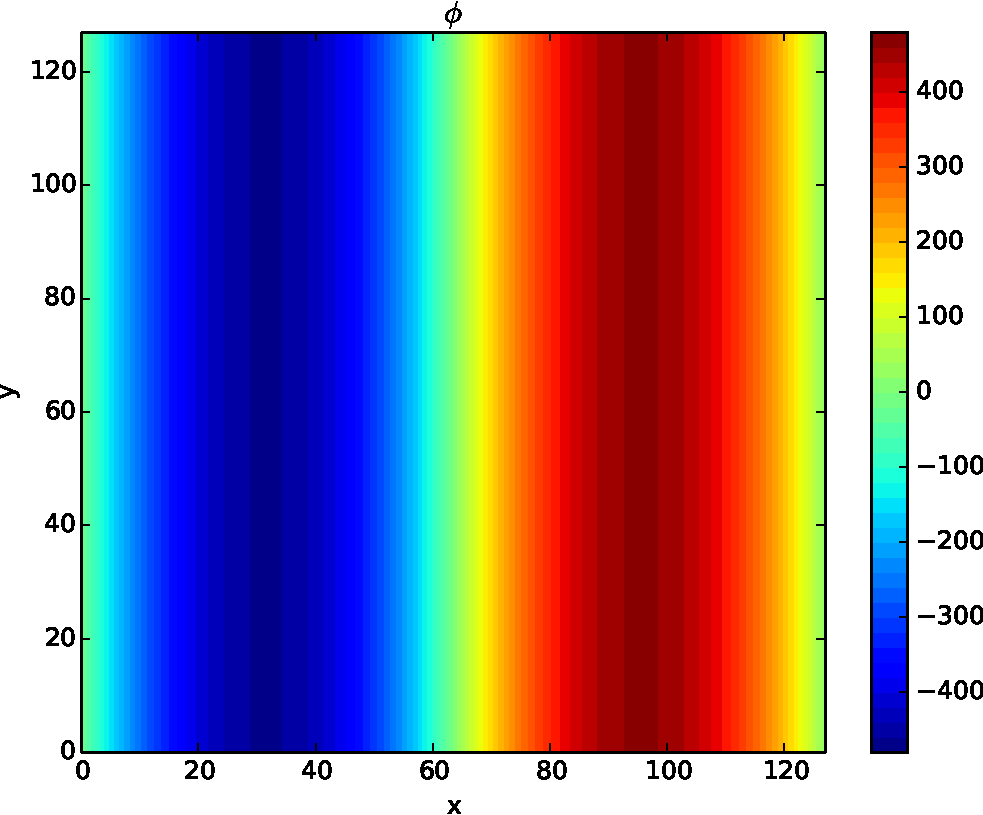
\includegraphics[width = \textwidth]{figures/verification/heaviside/phi.pdf}
	% 			% \end{subfigure}
	% 			% \begin{subfigure}[b]{0.32\textwidth}
	% 			% 	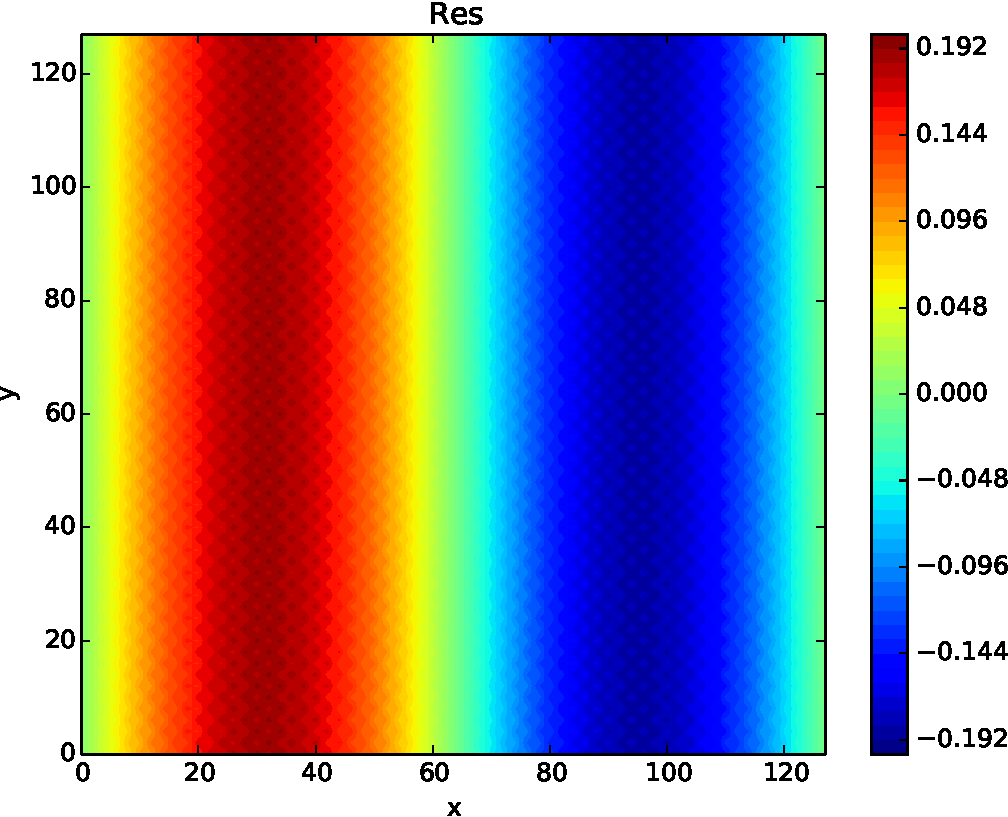
\includegraphics[width = \textwidth]{figures/verification/heaviside/residual.pdf}
	% 			% \end{subfigure}
	% 		\caption{As earlier this is a \(x,y\)-plane cut along \(x_k=32\), of the grid. The plots show the charge distribution,
	% 		numerical solution and the solution, from left to right. This is a test case constructed
	% 		with Heaviside functions. In the solution of the potential the expected second degree polynomial can be seen.
	% 		}
	% 		\label{fig:heaviside}
	% 	\end{figure}
	%
	% 	\subsection{Random Charge distribution}
	% 		To hopefully avoid some problems, that could appear due to the earlier test
	% 		cases being to constructed being to orderly, a test with a randomized
	% 		charge distribution is also included. The \cref{fig:random} shows the
	% 		charge distribution, numerical potential and the residual. The mean residual was
 % 			found to be \(\bar{r} \approx 0.00388\).
	% 		%
	% 		\begin{figure}
	% 			\centering
	% 			% \begin{subfigure}[b]{0.32\textwidth}
	% 			% 	\includegraphics[width = \textwidth]{figures/verification/random/rho.pdf}
	% 			% \end{subfigure}
	% 			% \begin{subfigure}[b]{0.32\textwidth}
	% 			% 	\includegraphics[width = \textwidth]{figures/verification/random/phi.pdf}
	% 			% \end{subfigure}
	% 			% \begin{subfigure}[b]{0.32\textwidth}
	% 			% 	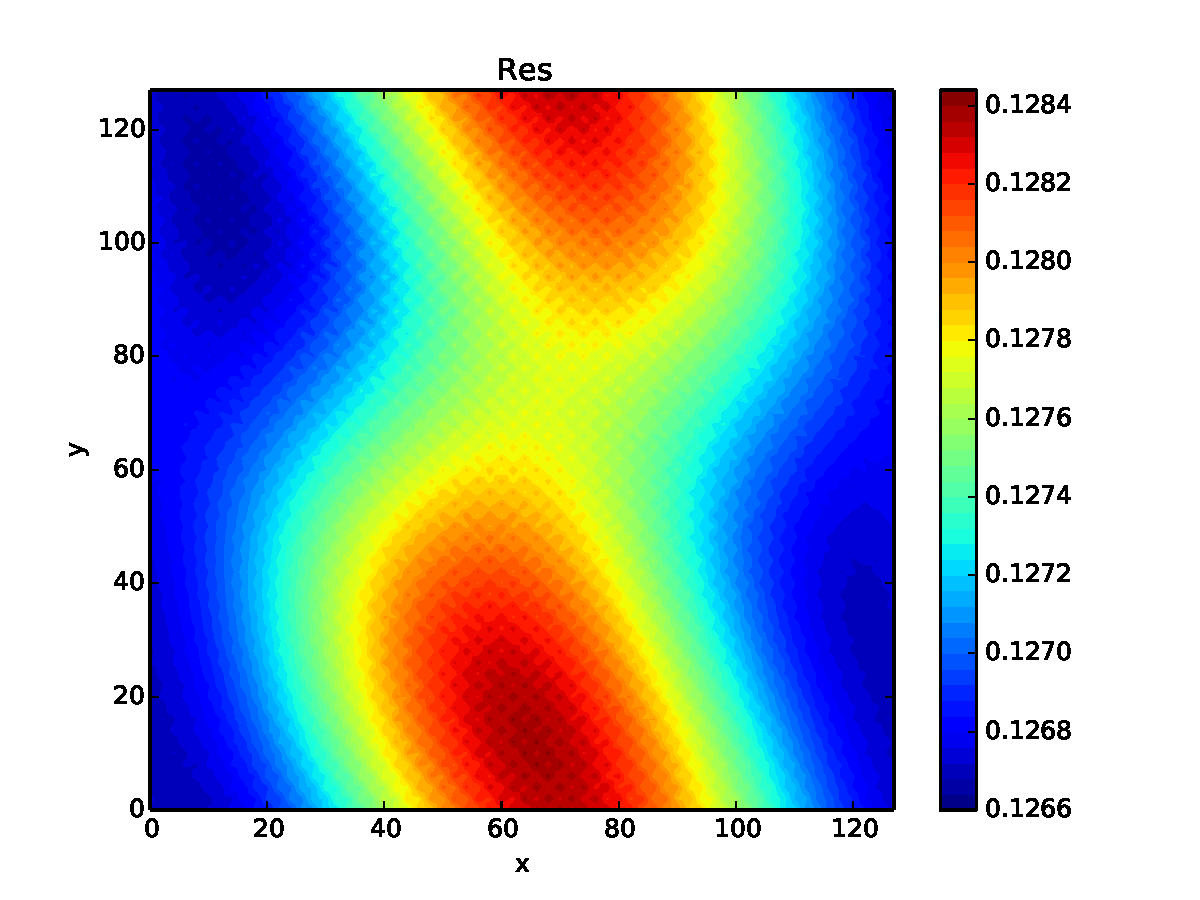
\includegraphics[width = \textwidth]{figures/verification/random/residual.pdf}
	% 			% \end{subfigure}
	% 			\caption{As earlier this is a \(x,y\)-plane cut along \(x_k=32\), of the grid. The plots show the charge distribution,
	% 			numerical solution and the solution, from left to right.}
	% 			\label{fig:random}
	% 		\end{figure}
%
% \section{Multigrid Solver}
% 	To test the solver itself we employ a couple different techniques. First we
% 	create a charge distribution by differentiating a known potential, and then
% 	running the solver and check if the resulting potential was equal to the original
% 	known potential.
%
% 	For the second test we use a charge distribution with a known analytical solution,
% 	and we then check that the solver reproduces the known analytical solution.
%
% 	A third method we use to verify it is to produce a random charge potential
% 	and then check that the potential converges, or in other words
% 	that the residual goes toward zero.
%
% 	Then lastly we use the solver on identical charge distributions with the domain
% 	divided up into different subdomains and check that the solver produces the same
% 	potential.
% \subsection{Predetermined Potential}
% 		In this section we first decide which potential we want, then numerically
% 		construct a corresponding charge potential by derivating. Then we compare the
% 		result with the original potential.

		% In
		%
		% \begin{figure}
		% 	\centering
		% 		\begin{subfigure}
		% 	% 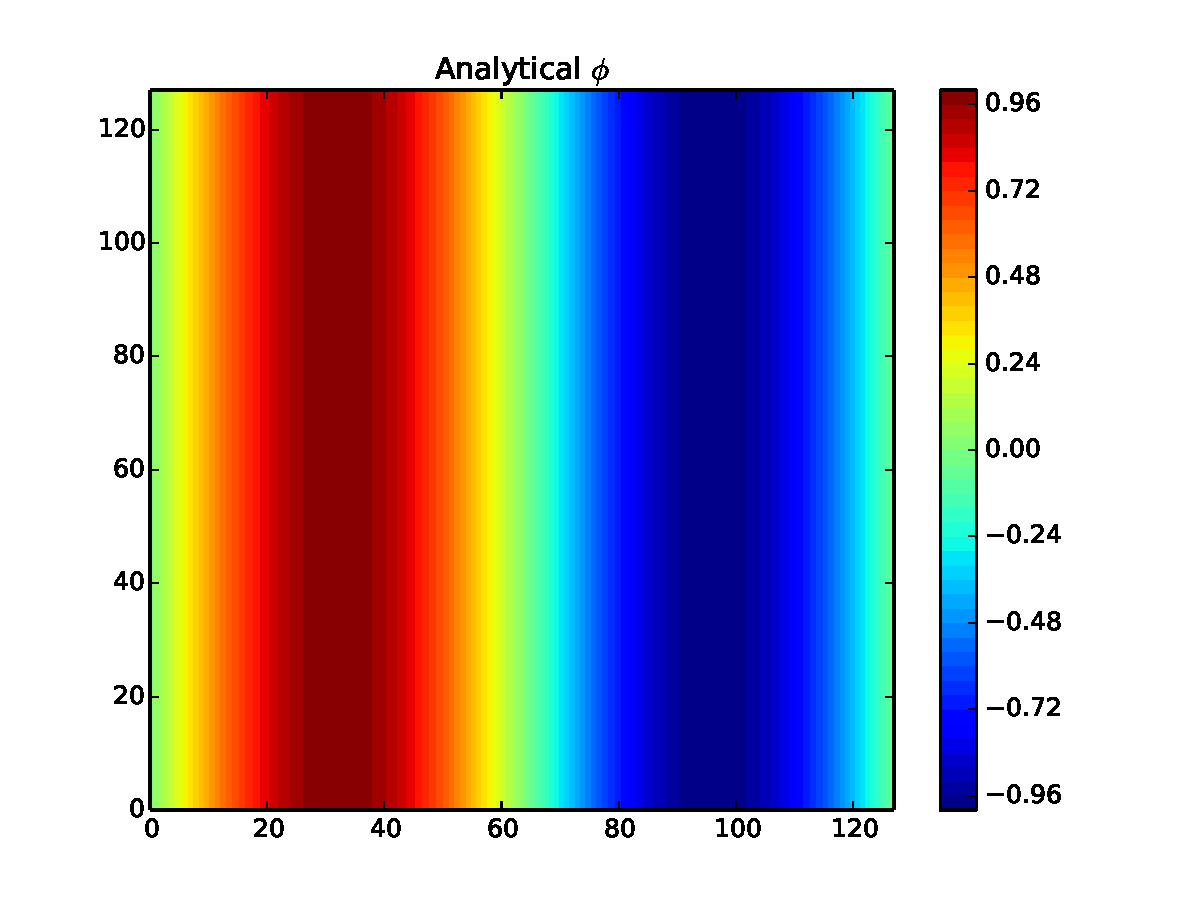
\includegraphics[width = 0.45\textwidth]{figures/verification/sinusoidal/analytical.pdf}
		% 	\end{subfigure}
		% 		\begin{subfigure}
		% 	% 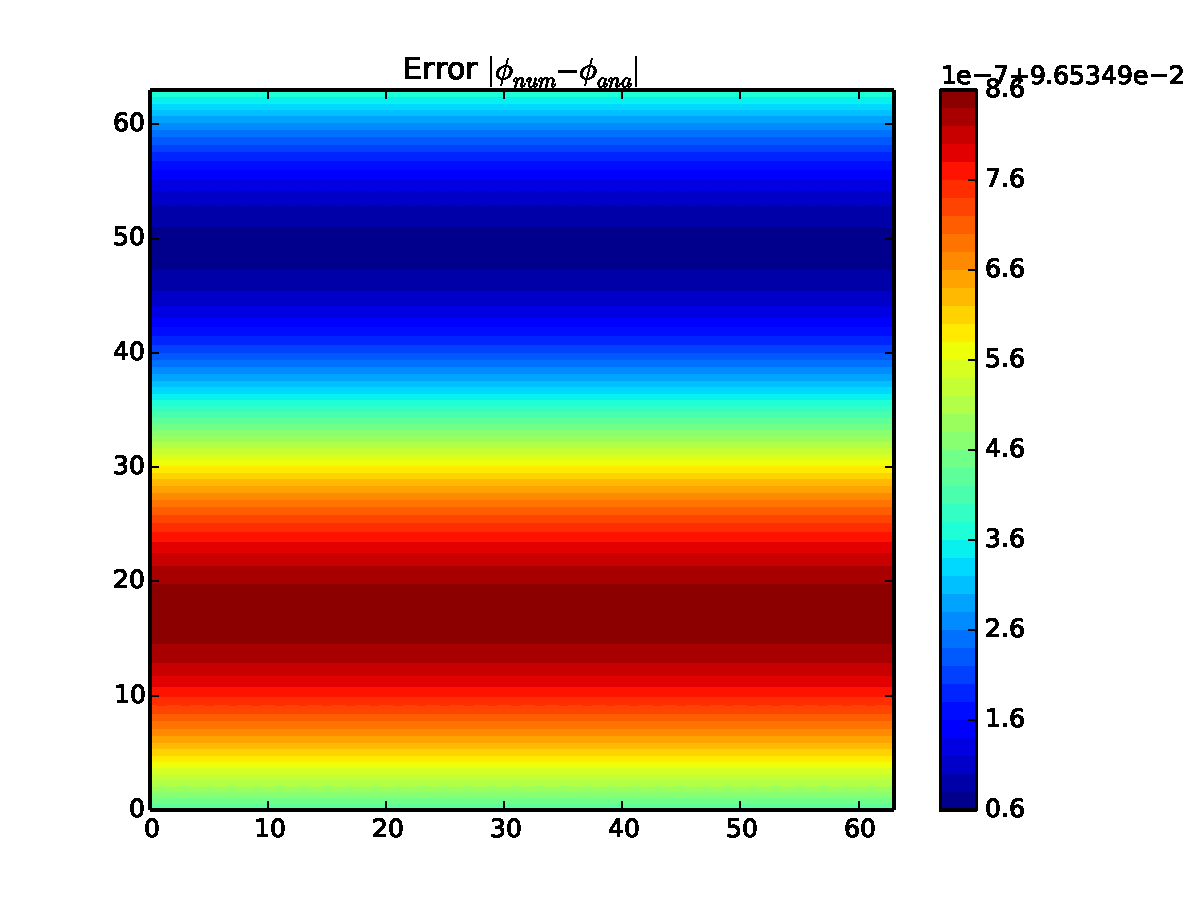
\includegraphics[width = 0.45\textwidth]{figures/verification/sinusoidal/error.pdf}
		% \end{subfigure}
		% \end{figure}
		%

		\subsection{Convergence of Residual}
		(TBD)

		\subsection{Different Domain divisions}
		(TBD)

% \section{Particle-in-Cell}
%
% 	\subsection{Plasma Oscillations}
%
% \textbf{NB! See if something below is salvageable}
%
%
% The multigrid method has several different steps in the algorithm, as a developmental
% help and to ensure that the program works correctly during as many different conditions
% as possible we want to test the whole code, as well as the constituent parts where possible.
% The method is quite modular and several parts of it can be tested alone.
% The GS-RB, used for smoothing, can be independently tested, since on it's own it converges to a solution,
% just at a higher computational cost than the multigrid method. To test it we will
% use an initial density field with a length between the grid steps that results in
% an exact answer. The restriction and prolongation operators can also tested to a
% degree by checking that they preserve a constant grid through several grid level changes.
%
%
% The multigrid method has several different steps in the algorithm, as a developmental
% help and to ensure that the program works correctly during as many different conditions
% as possible we want to test the whole code, as well as the constituent parts where possible.
% The method is quite modular and several parts of it can be tested alone.
% The GS-RB, used for smoothing, can be independently tested, since on it's own it converges to a solution,
% just at a higher computational cost than the multigrid method. To test it we will
% use an initial density field with a length between the grid steps that results in
% an exact answer. The restriction and prolongation operators can also tested to a
% degree by checking that they preserve a constant grid through several grid level changes.
%
% \subsection{The Multigrid method}
% 	We use both of the aforemented tests to check that the whole multigrid method
% 	works as intended. Since a constant source term will give a trivial solution of
% 	the potential, \(\phi(x,y,z) = \va{0}\), we use that as a test. In addition we
% 	also test that it converges on a sinusoidal source term as we did the smoother.
%
%
% \subsection{Smoothers}
%
% 	The iterative method GS-RB used for the pre- and postsmoothing of the grid in
% 	our implementation of the multigrid method is also a direct solver.
% 	So we can test it, or most other smoothers, by testing them on a small system
% 	where the problem has an analytical solution. Then we can let them run for a
% 	while and ensure that they are converging towards the solution. If we let
% 	the source term be sinusoidal in one direction, and constant in the other
% 	directions it has an easy solution given below
%
% 	\begin{align}
% 		\nabla^2 \phi(x,y,z) &= \sin(x)
% 	\end{align}
%
% 	This has a solution when \(\phi(x,y,z) = -\sin(x)\) and we can test that the
% 	solver converges to the solution. If we let the source term be constant in the
% 	x direction and instead vary in the other directions we can get verify that the
% 	solver works in all three directions independently.

    In this chapter we will go through different methods we used to verify the multigrid
solver, as well as scaling measurements. Modular parts of the solver is tested with unittests
where feasible. In addition the whole solver is tested with both analytically solvable
test cases and randomly generated fields.


\subsection{Error Quantification}
	\label{sec:errorQuant}
    (NOTE TO SELF: Tidy up)
	In order to evaluate solutions we will primarily look at the normalized 2-norm of the error, \cref{eq:2norm},
	and the residual, \cref{eq:barRes}. The \(\norm{ err }_2\) is computed from comparing the numerical
	solution \(\hat{\phi}\) to an analytical solution \(\phi\) and normalized with regards to grid points, \(N\).
	The residual is found by inserting the numerical solution into the Poisson equation, the remaining
	part is then the residual, and shows the difference of the current numerical solution
	and the optimal numerical solution.
	%
	\begin{align}
		\norm{ err }_2&= \sqrt{\frac{\sum \left(\hat\phi - \phi\right)^2}{N}}  \label{eq:2norm}
		\\
		\bar{r} &= \frac{1}{N}\left( \sum_i{ \nabla^2 \hat{\phi}_i + \rho_i  }  \right) \label{eq:barRes}
	\end{align}

    \section{Multigrid Solver}
	To test the solver itself we employ a couple different techniques. First we
	create a charge distribution by differentiating a known potential, and then
	running the solver and check the difference to the original potential.

	For the second test we use a charge distribution with a known analytical solution,
	and we then we compare the numerical solution to the analytical solution.

	Since constructed solutions can often behave to nice, we will also perform
	a third test on a randomized charge distribution, here we will only look at the
	residual since we cannot compute the error due to not having an analytical solution.
	We expect the residual to approach \(0\).

	Lastly we perform a few run on identical charge distributions, domain subdivisions
	and compare the solutions.

% \subsection{Predetermined Potential}
% 		In this subsection a potential is first constructed, then numerically differentiate
% 		it to obtain a charge distribution. Then we will let the program solve the
% 		problem and compare the numerically obtained potential with the original potential.
%
% 		\begin{figure}
% 			\centering
% 			\begin{subfigure}[b]{0.45\textwidth}
%                     % \missingfigure[figwidth=\textwidth]{Blank}
% 			% 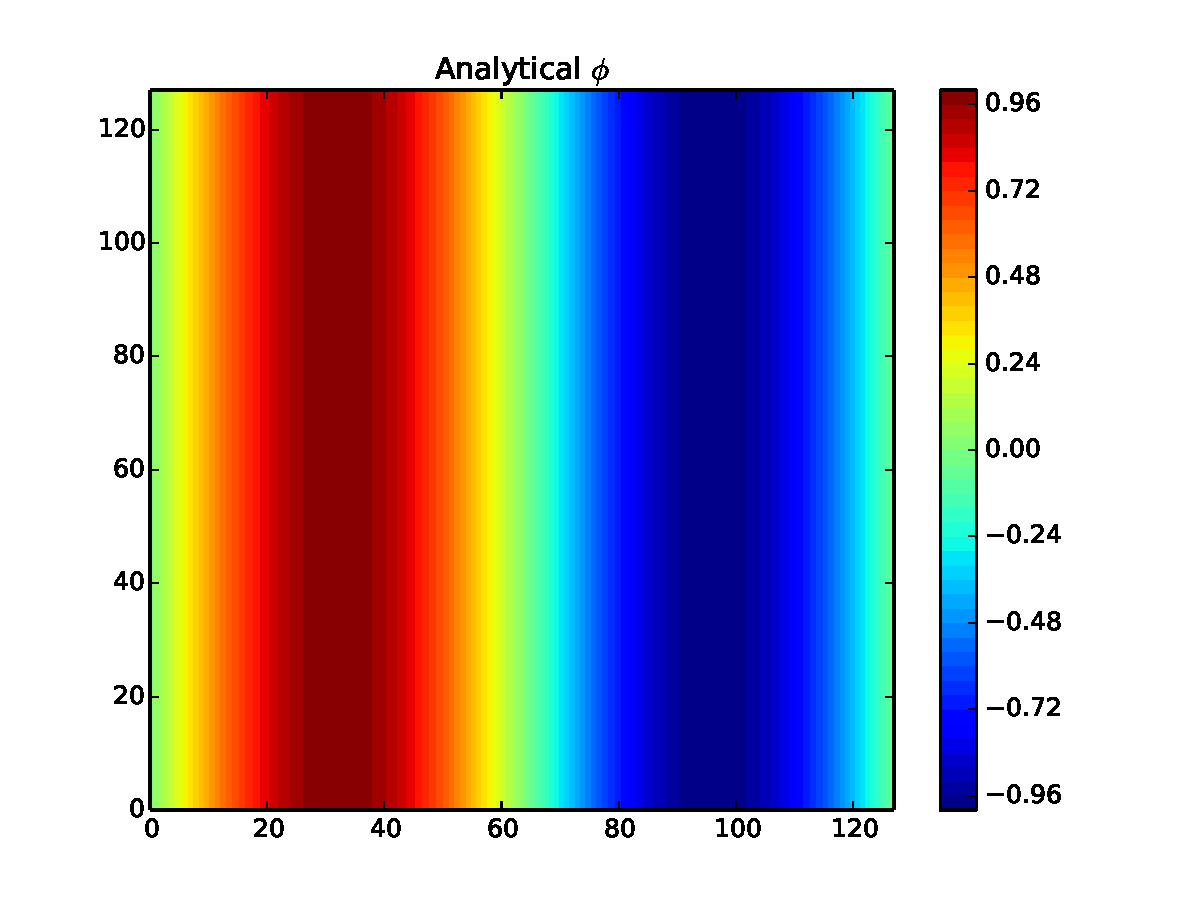
\includegraphics[width = 0.45\textwidth]{figures/verification/sinusoidal/analytical.pdf}
% 			\end{subfigure}
% 			\begin{subfigure}[b]{0.45\textwidth}
%                     \missingfigure[figwidth=\textwidth]{Blank}
% 		% 	% 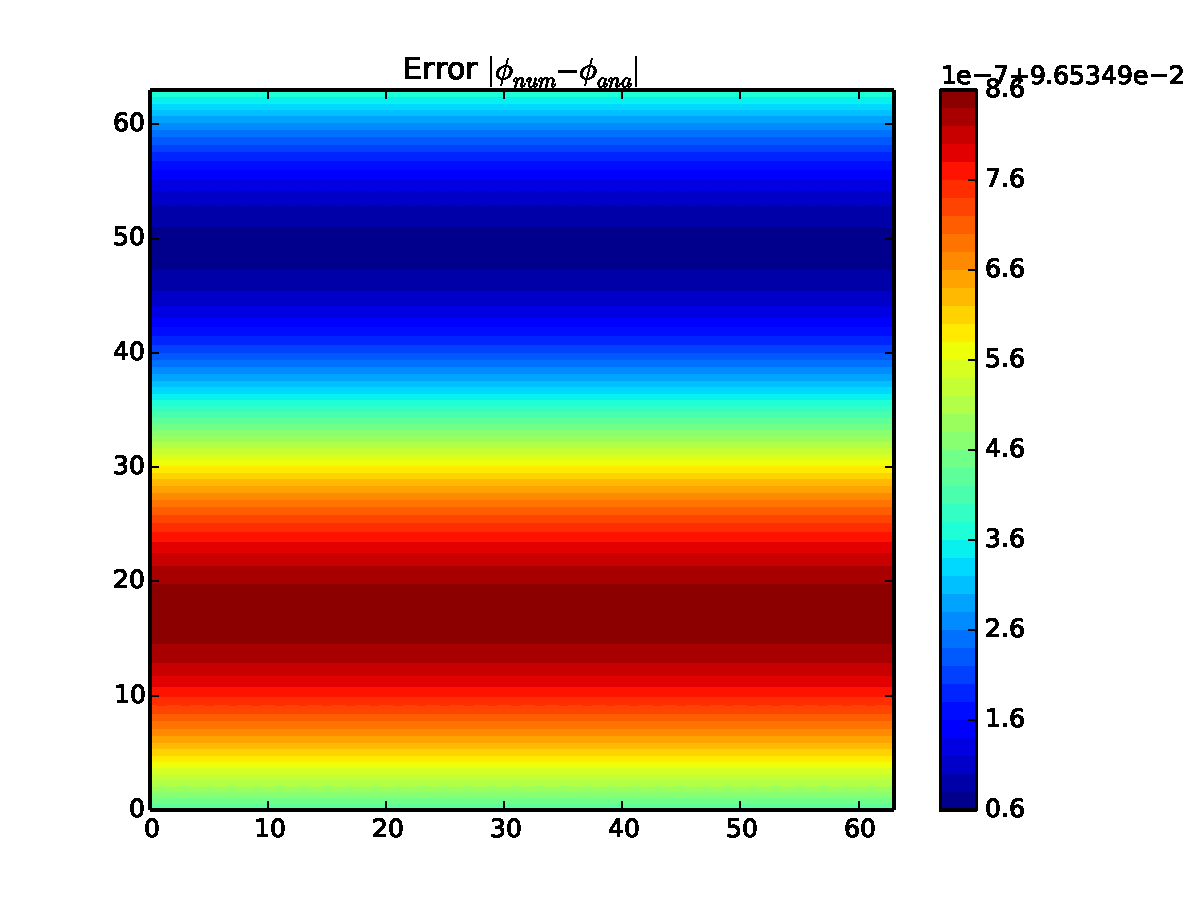
\includegraphics[width = 0.45\textwidth]{figures/verification/sinusoidal/error.pdf}
% 		\end{subfigure}
% 		% \caption{}
% 		\end{figure}




\subsection{Analytical Solutions}
	We use a few different constructed charge density fields, which is analytically solvable,
	to test the performance and correctness of the solver. All the simulations here are ran on
	a grid of the size \( 128, 64, 64 \) divided into \(1,2,2\) subdomains, with pinc
	version 36ad.
		It uses \(5\) cycles when presmoothing, solving on the coarsest grid and postsmoothing, the
	MG solver is instructed to run for \(100\) MG V-cycles with \(2\) grid levels.

\subsubsection{Sinusoidal function}
	\label{sec:sinusoidal}
	A sinusoidal source term, \(\rho\) can be useful to test the solver since
	it can be constructed to have very simple derivatives and integrals. Here
	we use a sinusoidal function that has two positive tops and two negative tops
	over the total domain. We want the sinus function to go over \(1\) period
	over the domain, so we normalize the argument by dividing the grid point
	value, \(x_j, y_k, z_l\), by the domain length in the direction, \(L_x, L_y, L_z\).

	\begin{align}
		\rho(x_j,y_j,z_l) &= \sin\left( x_j \frac{2\pi}{L_x} \right)\sin\left( y_{k} \frac{2\pi}{L_y} \right)
		\intertext{A potential that fits with this is:}
		\phi(x,y,z) &= -\left(\frac{2\pi}{L_x}\right)^2\left(\frac{2\pi}{L_y}\right)^2
			\sin\left( x_j \frac{2\pi}{L_x} \right)\sin\left( y_{k} \frac{2\pi}{L_y} \right)
	\end{align}

	\begin{figure}
		\centering
			\begin{subfigure}[b]{0.32\textwidth}
				\includegraphics[width = \textwidth]{figures/verification/analytical/sinusoidal/rho.pdf}
			\end{subfigure}
			\begin{subfigure}[b]{0.32\textwidth}
				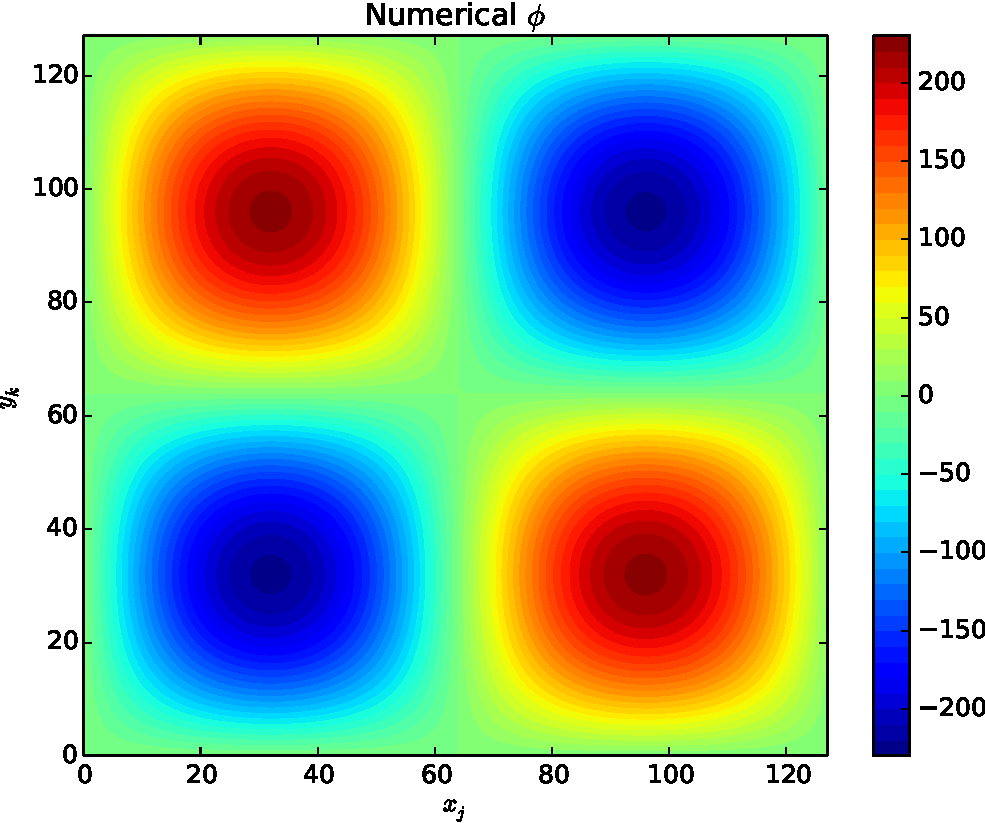
\includegraphics[width = \textwidth]{figures/verification/analytical/sinusoidal/numerical.pdf}
			\end{subfigure}
			\begin{subfigure}[b]{0.32\textwidth}
				\includegraphics[width = \textwidth]{figures/verification/analytical/sinusoidal/residual.pdf}
			\end{subfigure}
		\caption{This a \(x,y\)-plane from the grids cut along \(z_l = 32\), from the sinusoidal test case described in \cref{sec:sinusoidal}.
		The left plot shows the charge distribution, the center plot shows the numerical solution of the potential and the plot to the right depicts
		the residual.}
		\label{fig:sinusoidal}
	\end{figure}

	The \cref{fig:sinusoidal} shows the results from running the MG-solver on the test sinusoidal test case described here.
	As can be expected the potential mirrors the charge distribution, except with an opposite sign and a larger amplitude.
	A decently large grid was simulated and the mean residual was found to be: \(\bar{r} \approx 0.0312\).


	\subsubsection{Heaviside Function}
		The solver is also tested with a charge distribution governed by a Heaviside
		function. This is also suited to testing since the charge distribution is then
		constant planes, and we expect second order polynomial when integrating them.
		In the test case there are two planes with the value \(-1\) and two
		planes with \(1\). In \cref{fig:heaviside} the test case, as well as the solution and residual is
		shown, and we can see the polynomials in the solution. The mean residual \(\bar{r}\) was
		\(0.00677\).

	\begin{align}
		\rho_(x_j,y_k,z_l) &= \begin{cases} 1  & y_j \epsilon (0, 32), (64,96)\\ -1  & y_j \epsilon (33, 65), (97,127) \end{cases}
	\end{align}

	\begin{figure}
		\centering
        \missingfigure{Blank}
			\begin{subfigure}[b]{0.32\textwidth}
				\includegraphics[width = \textwidth]{figures/verification/analytical/heaviside/rho.pdf}
			\end{subfigure}
			\begin{subfigure}[b]{0.32\textwidth}
				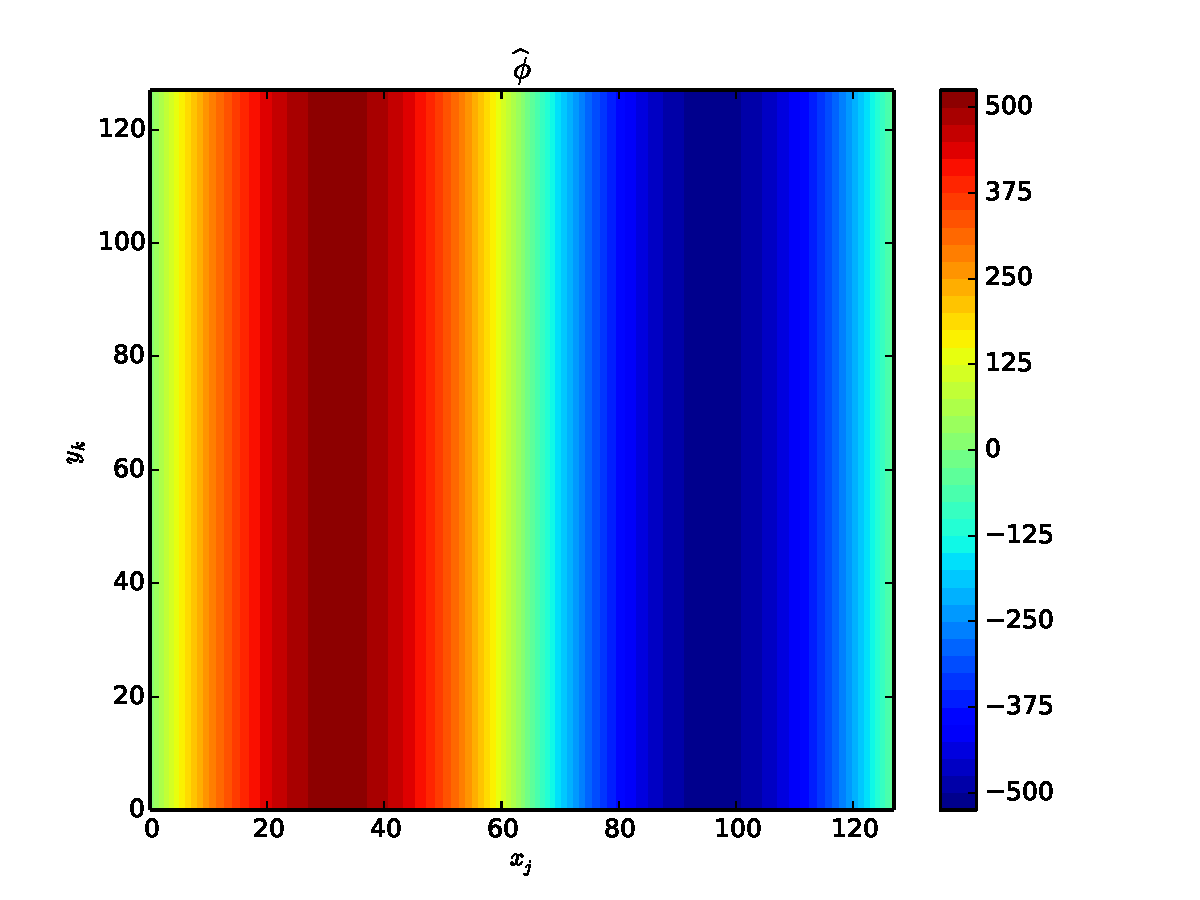
\includegraphics[width = \textwidth]{figures/verification/analytical/heaviside/numerical.pdf}
			\end{subfigure}
			\begin{subfigure}[b]{0.32\textwidth}
				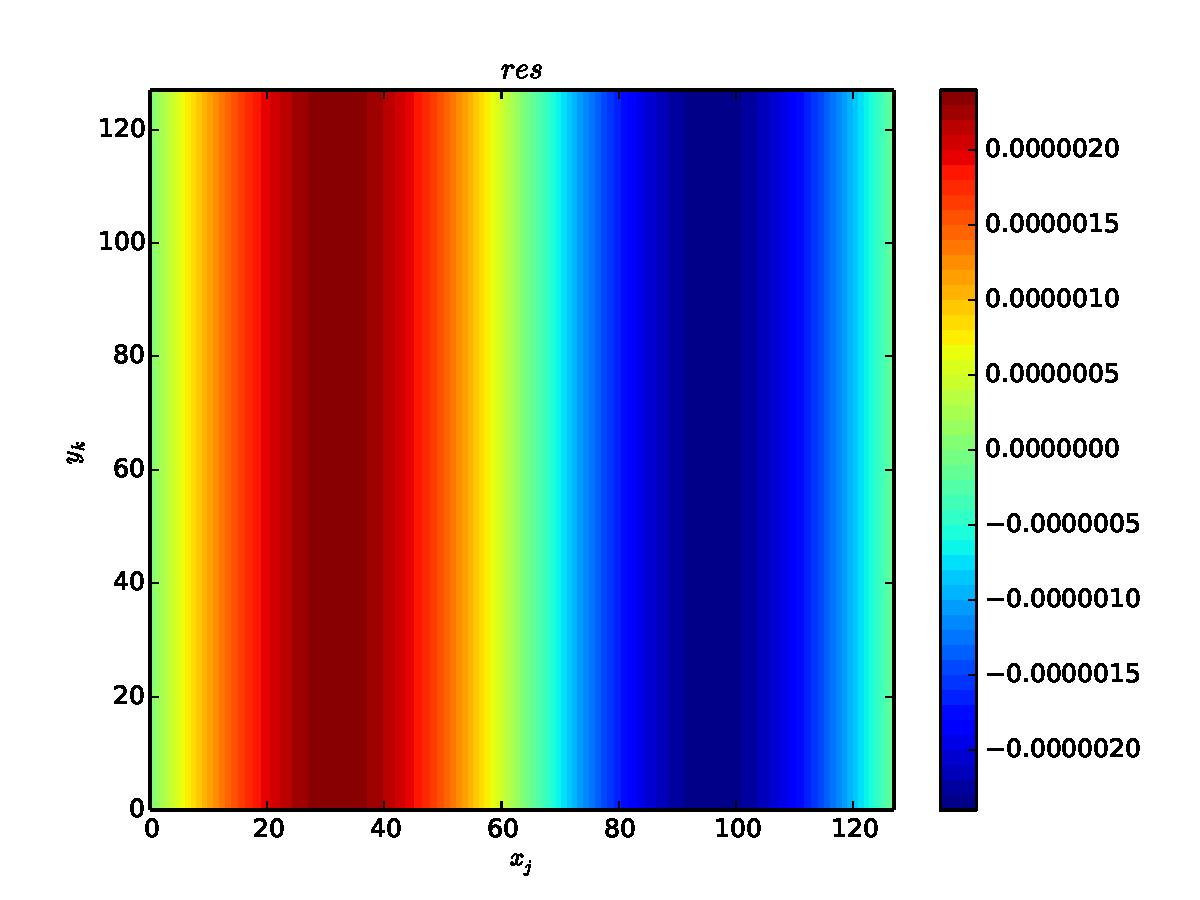
\includegraphics[width = \textwidth]{figures/verification/analytical/heaviside/residual.pdf}
			\end{subfigure}
		\caption{As earlier this is a \(x,y\)-plane cut along \(x_k=32\), of the grid. The plots show the charge distribution,
		numerical solution and the solution, from left to right. This is a test case constructed
		with Heaviside functions. In the solution of the potential the expected second degree polynomial can be seen.
		}
		\label{fig:heaviside}
	\end{figure}

	\subsection{Random Charge distribution}
		To hopefully avoid some problems, that could appear due to the earlier test
		cases being to constructed being to orderly, a test with a randomized
		charge distribution is also included. The \cref{fig:random} shows the
		charge distribution, numerical potential and the residual. The mean residual was
			found to be \(\bar{r} \approx 0.00388\).
		%
		\begin{figure}
			\centering
            \missingfigure{Blank}
			\begin{subfigure}[b]{0.32\textwidth}
				\includegraphics[width = \textwidth]{figures/verification/analytical/random/rho.pdf}
			\end{subfigure}
			\begin{subfigure}[b]{0.32\textwidth}
				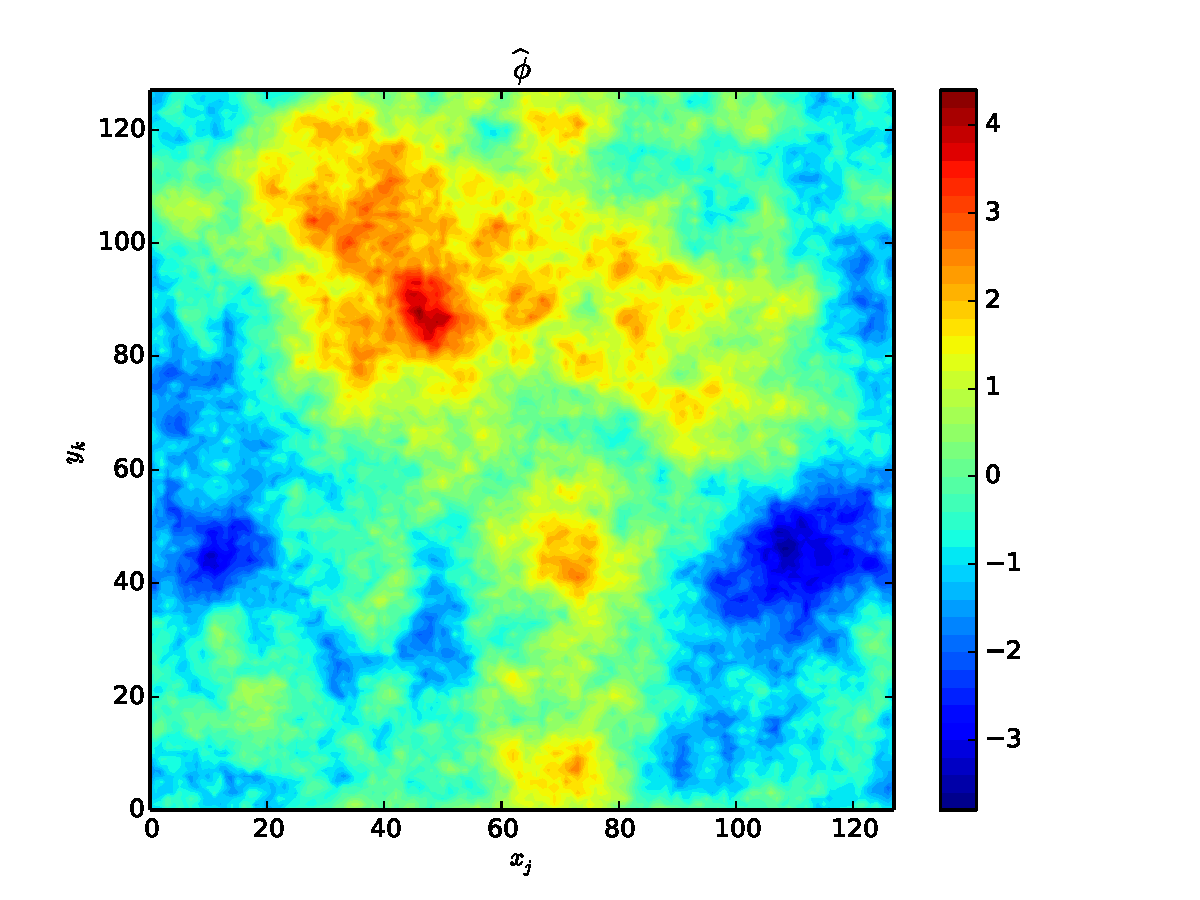
\includegraphics[width = \textwidth]{figures/verification/analytical/random/numerical.pdf}
			\end{subfigure}
			\begin{subfigure}[b]{0.32\textwidth}
				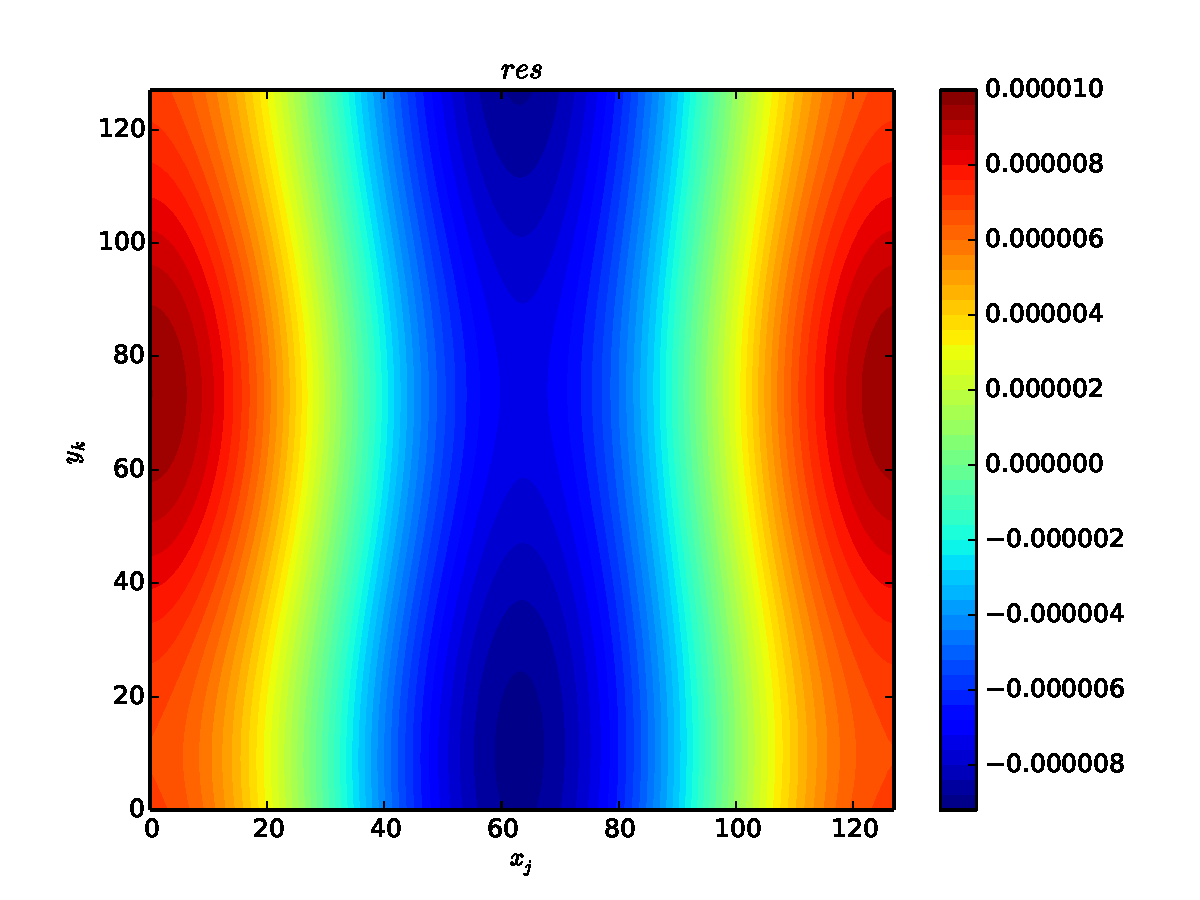
\includegraphics[width = \textwidth]{figures/verification/analytical/random/residual.pdf}
			\end{subfigure}
			\caption{As earlier this is a \(x,y\)-plane cut along \(x_k=32\), of the grid. The plots show the charge distribution,
			numerical solution and the solution, from left to right.}
			\label{fig:random}
		\end{figure}

    \section{Scaling of the error compared to discretization}
The charge density is represented by a discretized grid, due to this a numerical solution
will have an inherent error.
The error will be of second order, \(\order{h^{-2}}\), dependent on the
stepssize, \(\Delta x\), due to the first order solver, see \cref{sec:GSRB}.

To investigate that the error the of the solver follows a second order improvement
as the stepsize decreases we construct a sinusoidal \(rho\) as a test case.

\begin{equation}
    \rho(x) = \sin{\left(\frac{x}{2\pi}\right)}; \qquad x\epsilon[0,2\pi] \label{eq:sinus_errorScaling}
\end{equation}

This \(\rho\) is analytically solvable for the Poisson equation so we can compute the
\(2\)-norm of the error, \(\norm{err}_2\). Then we gradually decrease the stepsize
and obtain and compare the norm of the numerical solutions. Since the normalization in PINC
is normally done outside the multigrid solver, \(rho\) had to be suitably scaled
to the stepsize. We expect the error to be proportional to the squared stepsize, \(err(h) \approx Ch^2\), where \(C\) is a constant dependent on the geometry of the problem.
By taking the logarithm we obtain

\begin{equation}
    \log(err(h)) = 2\log(Ch)
\end{equation}

\cref{fig:errorScaling} shows the
the measured error when solving the sinusoidal charge distribution, \cref{eq:sinus_errorScaling},
for both the potential, \(\phi\), and the electric field, \(E_x\).
The problem was solved with different discretizations on a \(3\)-dimensional domain,
starting at \([8,8,8]\) doubling the grid points each time. The slope on the logarithmic plots
was in both cases found to be \(2.00\), showing a second order error scaling \(\order{h^{-2}}\).
The same test was also performed in \(1\) and \(2\) dimensional cases, with varying
subdomain configurations and with the sinus shape along the other axes.

\begin{figure}
    \centering
    \begin{subfigure}[b]{\textwidth}
        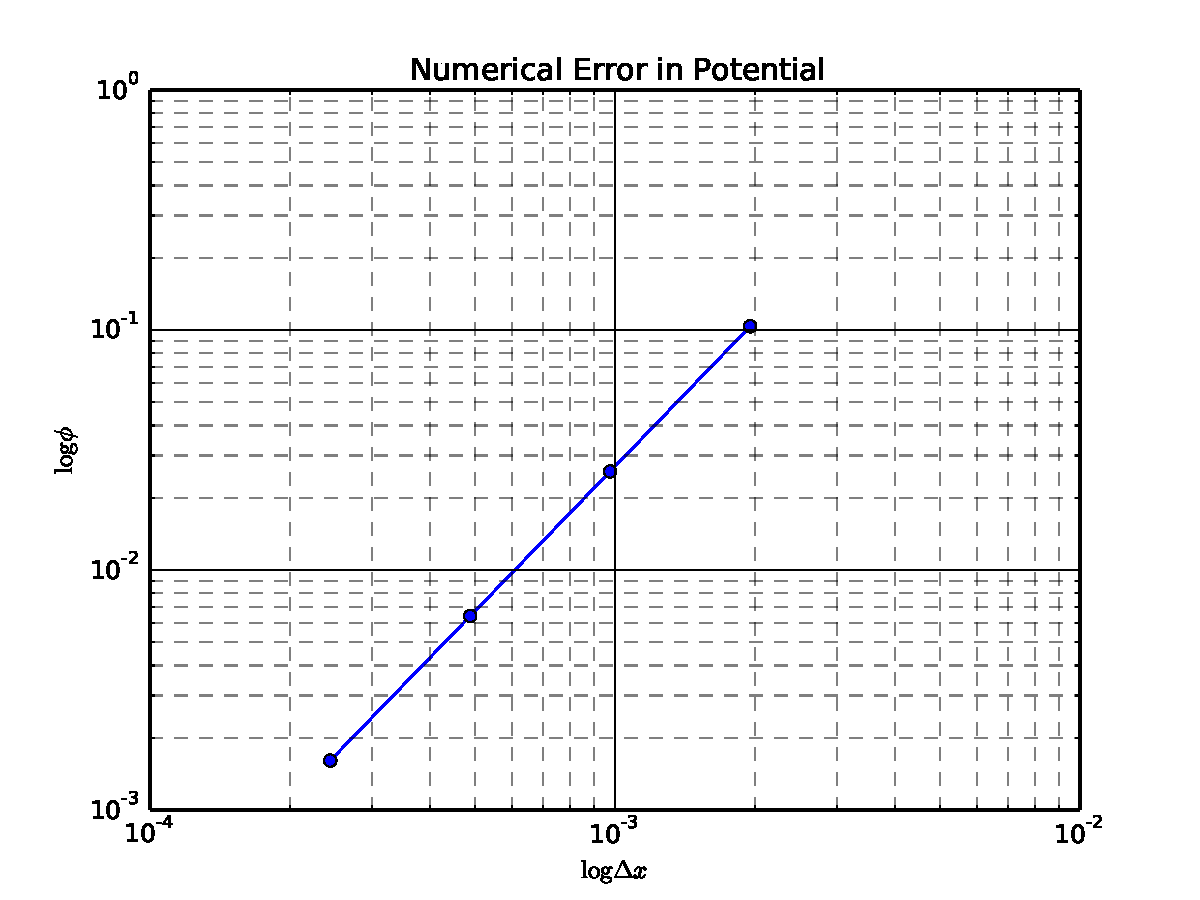
\includegraphics[width = \textwidth]{figures/verification/errorScaling/errorloglogPotential}
    \end{subfigure}
	\begin{subfigure}[b]{\textwidth}
		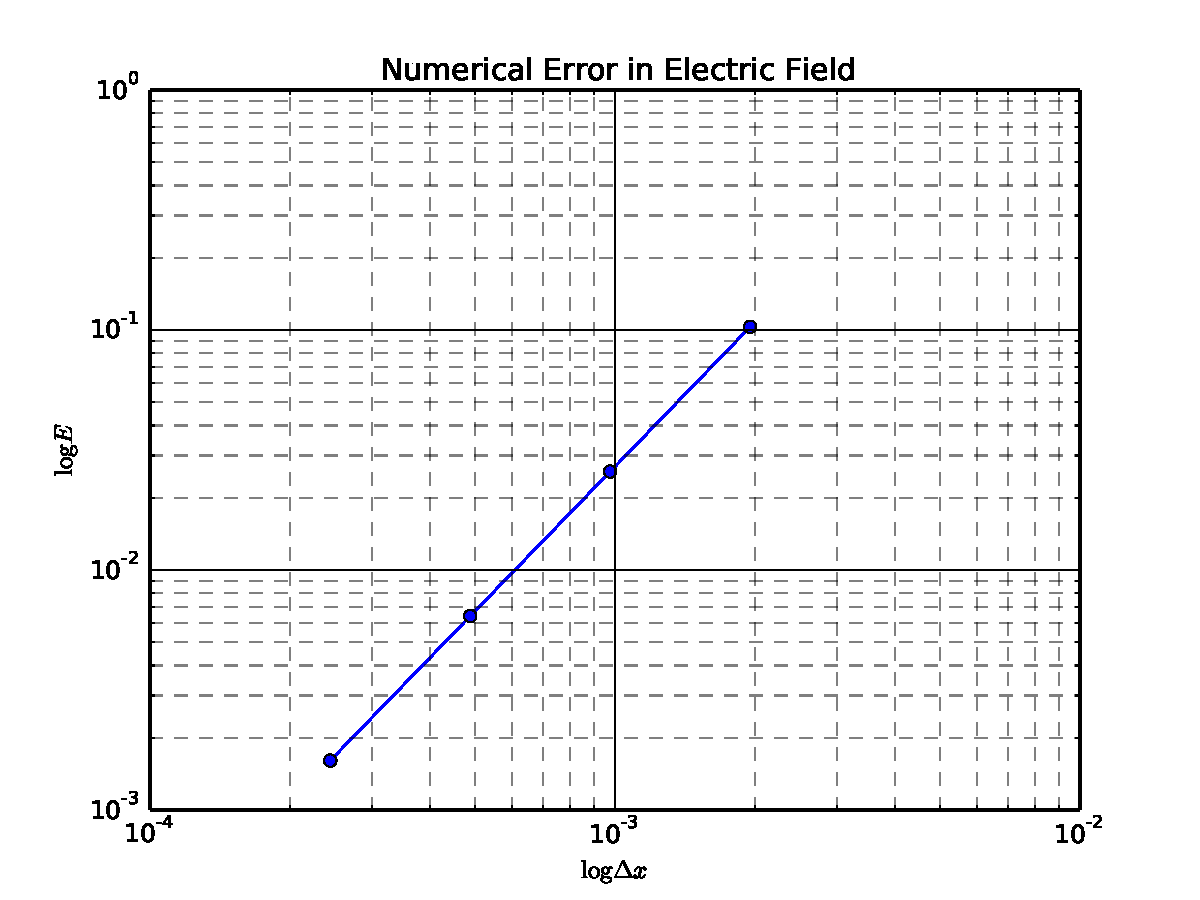
\includegraphics[width = \textwidth]{figures/verification/errorScaling/errorloglogE}
	\end{subfigure}
    \caption{Logarithmic plot of the 2-norm of the error of the potential \(\phi\), top figure, and the
    x-component of the electric field. The solver was run on a scaled sinus-shaped charge distribution.
    Both of the plots show a straight line of the error, on the logarithmic plots, with a slope
    of \(2.00\). This corresponds to the error scaling with order \(-2\) as a function of the
	stepsize. All the units are in PINC normalized units.}
    \label{fig:errorScaling}
\end{figure}

    \subsection{Langmuir Oscillation Test Case}
As a test of the validity of our PiC program, we can use the langmuir wave
oscillation. This test is inspired by a case set up in \citet{birdsall_plasma_2004},
and modified to fit with our normalization and discretizations.

    \section{Plasma Oscillation}
	\label{sec:langmuir_verification}
	As a test of the validity of our PiC program, we can use the Langmuir
	oscillation, described in \cref{sec:langmuir}.
	This test is inspired by a case set up in \citet{birdsall_plasma_2004},
	and modified to fit with our normalization and discretizations.
	To verify that the oscillation is properly simulated we will look at oscillations in the energy.


    \subsection{Input parameters}
        \subsubsection{Timestep}
        First we need to ensure that the simulation is does not violate the time-
        stability criterion, \cref{sec:time_stability}, \(\Delta t \leq 2\omega_{pe}\).
        For computational reasons each particle in the program represents many real particles
        and we can adjust the number, of real particles represented, to ensure
        that the electron plasma frequency is \(1\).

        \begin{equation}
            \omega_{pe}^2 = \frac{nq^2_e}{m\epsilon_0} = \left(\frac{N}{V}\right)\left(\frac{q_{e*}}{m_{e*} }\right)q_{e*}
        \end{equation}

        Here \((N/V)\) is just the number of electron super-particles divided by the volume,
        \(q_e\) and \(m_e\), represents super-particles and needs to be multiplied by the number
        of particles in a super-particle, \(\kappa\).

        \begin{equation}
            \omega_{pe}^2 = \left(\frac{N}{V}\right)\left(\frac{e}{m_e}\right)\kappa e
        \end{equation}

        Since we want the electron plasma frequency to be \(1\), \(\kappa\) is set to

        \begin{equation}
            \kappa = \frac{Vm_e}{Ne^2}
        \end{equation}

        Now the time is given in units of \(\omega_{pe}\) and we use \(\Delta t = 0.2 < 2\) easily.

        \subsubsection{Spatial-step}
        The spatial step need to satisfy the finite grid instability condition,
        \(\Delta x < \varsigma \lambda_{Se}\), \cref{sec:finite_grid_instability}.
        We use a similar procedure as in normalizing the time with regards to \(\omega_{pe}\)
        to normalize the length with regards to \(\lambda_{Se}\). The we end up with
        the temperature, or its other representation as thermal velocity, as the parameter we can adjust to make sure that it satisfies the
        condition.

        \begin{equation}
            \lambda_{Se}^2 = \frac{\epsilon_0 kT_e}{nq^2_e}
        \end{equation}

		% To make sure that

		\subsubsection{Simulation}
			We ran a simulation for \(10\tau_{pe}\), on a \(64,64,64\) size grid. The particles
			was first randomly distributed and given a maxwellian velocity distribution.
			Then they were slightly perturbed to create an imbalance.

			\begin{table}
					\center
			\begin{tabular}{c|c|c|c|c}
				Size 			&	Stepsize &	Timestep &\#Particles per cell	& \(v_{th}\) (electrons, ions)
				\\ \hline
				\((64,64,64)\)	& \(0.2\)	& \(0.1\)  	&	\(64\)	& 		\(0.002, 0.00046\)
			\end{tabular}
			\caption{Key settings for the langmuir wave oscillation. The complete settings are
			stored as an input file, langmuirWarm, in the PINC directory.}
			\end{table}

			The simulation were set to run for \(100\) timesteps, where each timestep represents \(0.1omega_{pe}^{-1}\).
			\begin{equation}
				\tau_p \equiv 2\pi/\omega_{pe}
			\end{equation}
			Using the plasma period this gives \(10/2\pi\approx 1.6\) periods.

		\begin{figure}
			\label{fig:oscillation}
			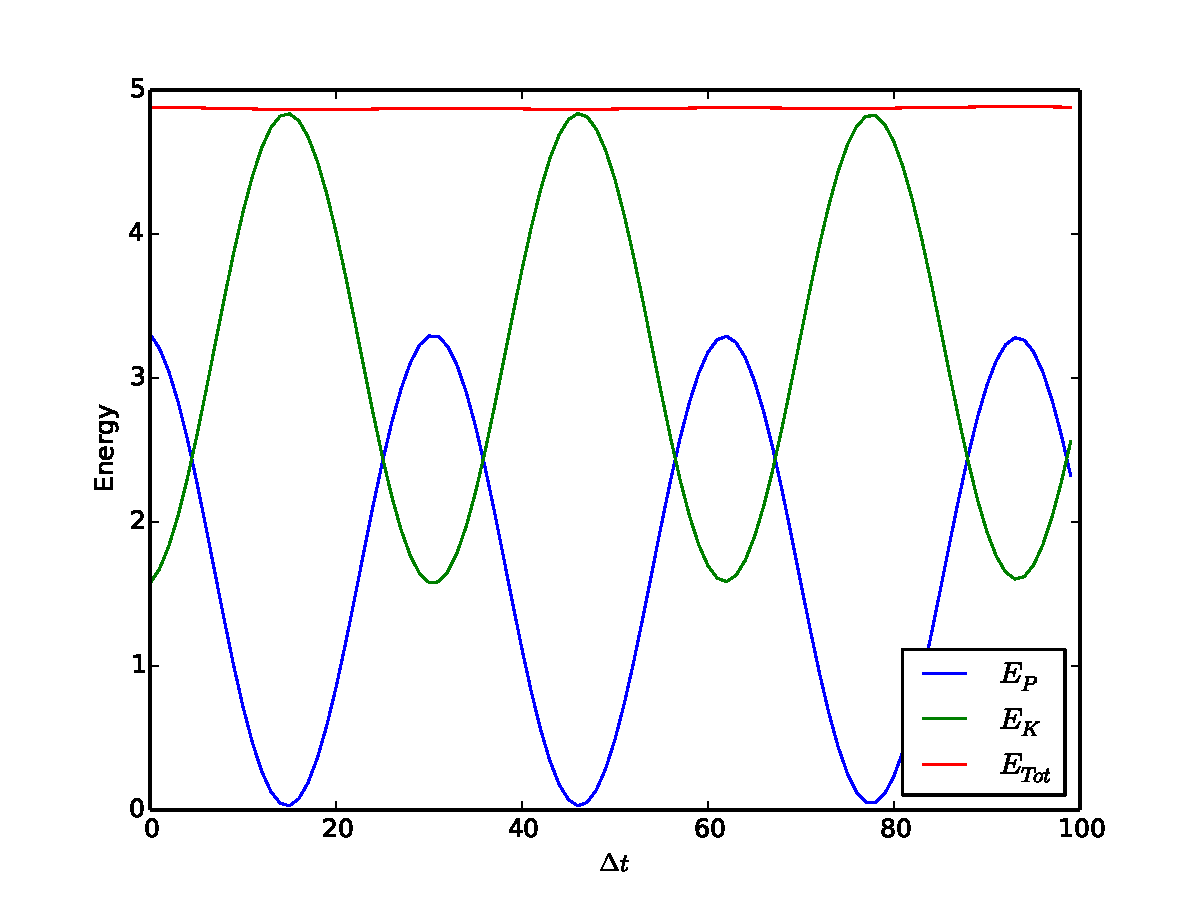
\includegraphics[width = \textwidth]{figures/verification/langmuirWave/energyPlot}
			\caption{This shows the time-evolution of the energy in an perturbed plasma. The energies are
			in normalized units and \(\Delta x = 0.1 \lambda_{De}\). The total energy has a maximum variation of \(0.22\%\). In the timespan
			of \(10\omega_{pe}\) the plasma oscillates over \(1.6\) times.}
		\end{figure}

		The \cref{fig:oscillation} shows the energy fluctuations for a plasma oscillation, the total energy
		is stable conserved, with a maximal variation of \(0.22\%\). The potential energy starts large
		and then it sinks as the potential energy is converted to kinetic energy. This is due to the particles
		attempting to neutralize the fields. The particles overshoots equilibrium position and the kinetic
		energy starts to convert back to potential energy.


\chapter{Performance/Results}
    \section{Scaling}
  In this section we investigate the performance of the solver and different scaling
  measurements. We are interested in both how well the solver performs on a larger
  number of processors, as well as the perfomance impact of the different
  parameters in the solver.

  We want to obtain a better understanding of how the field resolution can be scaled
  up without hampering the perfomance of the particle-in-cell simulation to much.

  

    \subsection{Convergence Rate}
	As an iterative solver a multigrid solver will gradually approach a solution,
	reducing the residual further each run. In this subsection we will measure the convergence
	rate, defined in similar way as in \citet{zhukov_parallel_2014},
	%
	\begin{equation}
		p = \left(\frac{r_m}{r_0}\right)^{1/m}
	\end{equation}
	%
	where \(r_m, r_0\) are the \(2\)-norm of a the residual after \(m\) multigrid runs
 	and the inital residual. We presume that each run of the multigrid solver will
	remove a proportion of the remaining residual.
	The tests are done on a sinusoidal
	problem for varying grid sizes. The smoothers run for \(100\) cycles on each of the \(5\) multigrid levels.
	%
	\begin{table}
	\centering
		\begin{tabular}{c|c|c}
			Grid 		& \(p\)
			\\ \hline
			\(64^3\)	& \(0.149\)
			\\ \hline
			\(128^3\)	& \(0.192\)
			\\ \hline
			\(256^3\)	& \(0.203\)
		\end{tabular}
		\caption{The convergence rate for the multigrid solver, running on \(5\) levels. The convergence rate becomes
		worse for larger grids.}
	\end{table}
	%
	\citeauthor{zhukov_parallel_2014} found convergence rates, \(p\), between  \( 0.095 \text{ and } 0.155\)
	using a multigrid solver with a Chebyshev algorithms to smooth. While the convergence rates found here were
	worse, this is to be expected with the much simpler Gauss-Seidel smoothers.

    \subsection{Scaling of the MG Solver}
	One of the aims of building a parallell multigrid solver was to be able
	to enable simulating large plasma problems. To be able to achieve that the solver
	should be able to scale up very well, i.e. doubling the problem size and the number
	of available processors should only give a manageable increase in computational time.
	We don't expect to be able to achieve a perfect parallelization, since there is
	a certain amount of interprocessor communications necessary that will slow down
	the algorithm compared to a sequential algorithm. The exact parallel performance
	is also dependent on the communications channels and the topology between the processor clusters.
	In \cref{sec:para_comp} the parallel
	complexeties for the different multigrd algorithms is given and we will look at
	the parallel proprties for a V, W and FMG algorithm.


	To investigate the scaling properties we will run set up a standard problem,
	and solve it with increasing resolutions. We keep the size of the domain unchanged but increase the resolution (reducing the spacing). We start with a \(32^3\) grid on
 	\(1^3\) computaional core, then we increase the problemsize to \(64^3\) on \(2^3\)
	and so on. These tests were run on Abel, UiO's computer cluster, and the technical details
	can be found at the web page \footnote{http://www.uio.no/english/services/it/research/hpc/abel/more/index.html (Accessed 2016-11-15)}.
	The results are shown on c\ref{fig:scalingMG}.
	%
	\begin{figure}
		% \begin{subfigure{\textwith}
		\label{fig:scalingMG}
		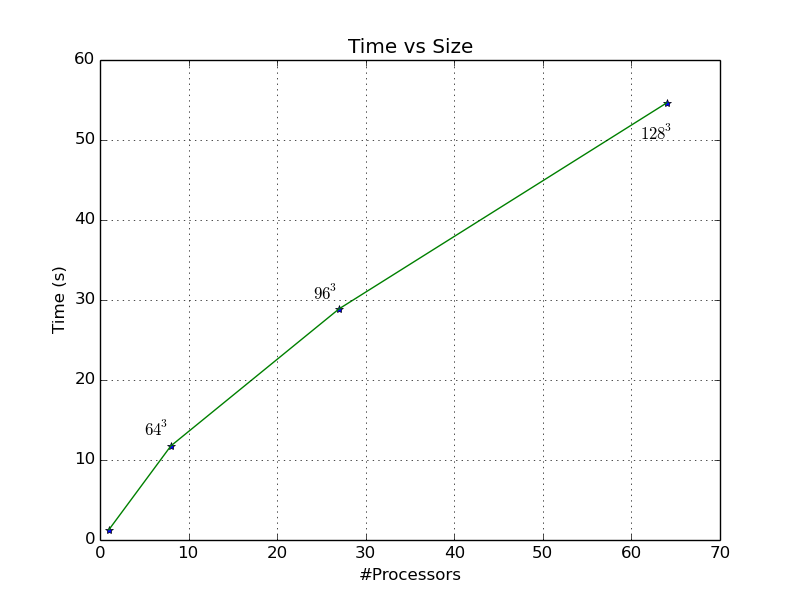
\includegraphics[width = \textwidth]{figures/performance/scalingMG}
		\caption{A Langmuir Oscillation were performed for \(10\) timesteps with a \((32,32,32)\) grid on each processor.
		This was repeated with increasing amount of processors, \((1, 8, 32, 64)\), to see how the multigrid solver scales.}
		% \end{subfigure}
	\end{figure}
	%
	%Comments
	From \cref{sec:para_comp} we expect theoretical optimal scaling of \(\log{N}\log{\varepsilon}\).
	While this was not achieved, the settings were not optimized in these runs, for the various problem sizes and
	this may have caused it to scale worse than it should. When more processors are used the speed of
	the interprocessor communcation may have slowed down, as the processors are not part of the
	same node. The main problem with the test was that the subdomains was very small so
	the communication costs dominated. The communication costs scales linearly \citep{jung_parallelization_1997}, so
	for the coarse grids of the \(5\)-level multigrid the solver scaled close to linearly.

	\citet{baker_scaling_2012} found it crucial to use assumed partition
	to achieve good scalability, as the interprocessor communication costs are the main obstacle to
	scalability for multigrid methods. By assumed partitioning the subdomains are divided into nearby groups
	to easy communication between them.

    \subsection{Scaling properties PiC}
	As well as the scaling properties of the multigrid solver a look at the
	whole PiC model is interesting. This helps us easier pinpoint where further
	optimizations efforts should be directed. We do not necessarilly except the
	the particle based algorithms to scale up to larger problems in the same
	rate as	the solver. So above a certain number of processors, or size, there may
	be a bottleneck.




% \chapter{Discussion}
%   Put in discussion here
%
% \chapter{Conclusions}
%   Put wonderful conclusions here...
%
\appendix
\chapter{Further Development}
    Here is a list of what possible improvements and extensions that we hope
is eventually developed in our PINC program. Our aim was to develop a solid, basic
and easy to use parallel PiC program, that is suited to further development. Our hope
is that this project eventually develops into a full scale open source PiC program.

\begin{itemize}
    \item Objects
    \item Adaptive mesh
    \item Realtime plasma vizualizations (ala Atomify)
    \item Full Electromagnetic PiC
    \item Compatibility with FEM (dolphin) as a solver
    \item Hybrid, add on possibility of fluid-species and molecular dynamics
    \item Spectral Solvers (Wish that was available for testing of other solvers)
    \item Variable Ghost Layers
    \item Various stencils, interpolation and discretizations of different orders
\end{itemize}

%
\chapter{Notation}
    \section{Notation}
  While the notation is described in the main text at its first instance, we have also included
  this small note on the notation used to make it easier to look up.
  Notation that are only used in locally in smaller sections are not included here.

  In the PinC project we have decided to try to keep different indexes tied different
  objects to help avoid confusion and increase readability. Since the \(i\) index is
  reserved for incrementing particles, the spatial \(x,y,z\)-indexes are \(j,k,l\) instead of the
  more usual \(i,j,k\). So to make the transition between this document and the code
  easier we have also used the \(j,k,l\) indexes to denote the spatial area.
  This is the convention used by Birdsall and Langdon, (cite plasma physics via simulation).


  Subscripts are usually used to denote spatial index, and a superscripts are usually
  reserved for temporal cases. So \( \Phi^n_{j,k,l} \) means the potential at
  the timestep \(n\) and position \(j,k,l\). When plasma theory is involved the subscript
  can also signify the particle species.


  \begin{centering}
    \begin{tabular}{c |l}
      \(\Phi\) & Electric Potential
      \\
      \(\rho\) & Charge Density
      \\
      \(\omega_{pe}\) & Electron Plasma Frequency
      \\
      \(\omega_{ce}\) & Electron Cycletron Frequency
      \\
      \(T_e\)   & Electron Kinetic Temperature
      \\
      \(\vb{E} \)   & Electric Field
      \\
      \(\vb{B}\)    & Magnetic Field
      \\
      \(\vb{r} \)   & Position
      \\
      \(m \)        & Mass
      \\
      \(T \)        & Kinetic Temperature
    \end{tabular}
  \end{centering}

%
\chapter{Unittests}
    \section{Unittests}
\label{sec:unittests}
Unittests are small tests that is used to check that the single pieces of the code
work as they should. This serves a dual purpose in developing a software project.
When a part of the code is developed it serves as a framework to create a standardized
test of the piece of code that can easily be repeated. The unit tests are not maintained
in the latest version of the software.
It also helps when developing the higher level algorithms, in that the unittests ensures
that the problem lies in the higher level algorithm and not in the lower level pieces
it uses. When implementing wider changes, for example datastructures, the unittests
can help making sure that the changes are not causing any unintended bugs. For
information of how to use the unittests see the documentation, \cite{documentation}.

\subsection{Prolongation and Restriction}
	The prolongation and restriction operators with the earlier proposed stencils
  will average out the grid points when applied. So the idea here is to set up a
  system with a constant charge density, \(\rho(\va{r}) = C\), and then apply a
  restriction. After performing the restriction we can check that the grid points
  values are preserved. Then we can do the same with the prolongation. While this
  does not completely verify that the operators work as wanted, it gives an indication
	that we have not lost any grid points and the total mass of the charge density should be conserved.

\subsection{Finite difference}
  The finite difference operators is tested by setting up a test
  field based on a polynomial on which the operator should give an exact answer for.
  For example if we have a quantity \(f(x) = 3x\), then a first order finite difference
  scheme will give \(\hat{\nabla}f(x) = 3\).

\subsection{Multigrid and Grid structure}
  We want the basic grid to be available through a grid datastructure and the stack
  of grids stored in the multigrid structure. To ensure that this will still work
  through changes in the the structs there is a simple unittest that uses a grid struct
  to set up a field, then it is changed in the multigrid struct. Then it confirms
  that the values in the grid struct is also changed.

\subsection{Edge Operations}
  In the communication between the subdomains, as well as in the treatment of
  boundary conditions, there is a group of functions dealing with slice operations.
  These are tested by putting assigning each subdomain different constant values,
  then different slice operations is performed.

%
\chapter{Examples}
    \section{Ex: 3 level V cycle, steps necessary}
	\label{sec:EX_V_Ccyles}
\begin{dingautolist}{192}
			\item Compute defect on grid \(0\), the finest grid:
		\begin{itemize}
			\item	\( \widehat{\phi}_0 = \mathcal{S}(\phi_0, \rho_0)\)
			\item 	\(d_0 = \nabla^2\widehat{\phi}_0 - \rho_0\)
			\item Restrict defect: \(\rho_1 = \mathcal{R}d_0 \) \nonumber
		\end{itemize}
	\item Compute defect on grid \(1\):
		\begin{itemize}
			\item \(\widehat{\phi}_1 = \mathcal{S}(\phi_1^0, \rho_1)\)
			\item \(d_1 = \nabla^2\widehat{\phi}_1 - \rho_1 \)
			\item Restrict defect: \(\rho_2 = \mathcal{R}d_1 \)
		\end{itemize}
	\item Solve Coarse Grid for correction \(\omega\)
		\begin{itemize}
			\item \( \phi_2 = \mathcal{S}(\phi_2^0, \rho_2)\)
			\item Interpolate as correction:\(\omega_1 = \mathcal{I}\phi_2\)
		\end{itemize}
	\item Add correction on level 1:
		\begin{itemize}
			\item \(\widetilde{\phi}_1 = \widehat{\phi}_1 + \omega_1\)
			\item \( \phi_1 = \mathcal{S}(\widetilde{\phi}_1, \rho_1)  \)
			\item Interpolate correction:\( \omega_0 = \mathcal{I} \phi_1\)
		\end{itemize}
	\item Compute solution.
		\begin{itemize}
			\item \(\widetilde{\phi}_0 = \widehat{\phi}_0 + \omega_0\)
			\item \( \phi_0 = \mathcal{S}(\widetilde{\phi}_0, \rho_0)  \)
		\end{itemize}
\end{dingautolist}

%
\chapter{Optional methods}
    


\section{MG-Methods}

	\subsection{FMG}
		\begin{itemize}
			\item 'Easy' to implement.
			\item Theoretically scales \(\order{N}\) \citep{Press1987}, in reality
			\item FMG and W cycles are usually avoided in massive parallel computers \citep{chow_survey_2006}, as they visit the coarsest grid often, due to:
				\begin{itemize}
					\item At the coarsest level the computation is fast, communication usually the bottleneck
					\item Coarsest grid may couple all the domain, needs global communication
				\end{itemize}
			\item Options to solve the coarse matrix \citep{chow_survey_2006}
				\begin{itemize}
					\item Direct solver: Sequential, if small problem may be done on each processor to avoid communication
					\item Iterative method, Gauss-Seidel. Can be parallelized
				\end{itemize}
			\item Will use G-S with R-B ordering, has good parallel properties
		\end{itemize}


\section{Other methods worth considering}
		\begin{itemize}
			\item MUMPS (MUltifrontal Massive Parallel Solver), tried and compared in \cite{Kacem2012}, slower than MG.
				\begin{itemize}
					\item Solves \(Au = \rho\) for a sparse matrix.
				\end{itemize}
			\item

		\end{itemize}














% \begin{figure}
% 		\center
% 		\begin{tikzpicture}[%
% 		    >=triangle 60,              % Nice arrows; your taste may be different
% 		    start chain=going below,    % General flow is top-to-bottom
% 		    node distance=6mm and 45mm, % Global setup of box spacing
% 		    every join/.style={norm},   % Default linetype for connecting boxes
% 		    ]
% 		% -------------------------------------------------
% 		% A few box styles
% 		% <on chain> *and* <on grid> reduce the need for manual relative
% 		% positioning of nodes
% 		\tikzset{
% 		  base/.style={draw, on chain, on grid, align=center, minimum height=4ex},
% 		  proc/.style={base, rectangle, text width=10em},
% 		  test/.style={base, diamond, aspect=2, text width=5em},
% 		  term/.style={proc, rounded corners},
% 		  % coord node style is used for placing corners of connecting lines
% 		  coord/.style={coordinate, on chain, on grid, node distance=6mm and 45mm},
% 		  % nmark node style is used for coordinate debugging marks
% 		  nmark/.style={draw, cyan, circle, font={\sffamily\bfseries}},
% 		  % -------------------------------------------------
% 		  % Connector line styles for different parts of the diagram
% 		  norm/.style={->, draw, lcnorm},
% 		  free/.style={->, draw, lcfree},
% 		  cong/.style={->, draw, lccong},
% 		  it/.style={font={\small\itshape}}
% 		}
% 		% -------------------------------------------------
% 		% Start by placing the nodes



% 		%Setting up the nodes on the side
% 		% \node [term, left=of SD] (quantum) { Compute  Quantumforce};
% 		% \node[coord, right=of last]	(around1){};



% 		%Draw new links between boxes
% 		% \draw [->,lcnorm] (SD.west) -- (quantum);

% 		\end{tikzpicture}
% 		\caption{Multigrid method}
% 		\label{fig:schematic}
% 	\end{figure}





	% \begin{figure}
	% 	\center
	% 	\begin{tikzpicture}[%
	% 	    >=triangle 60,              % Nice arrows; your taste may be different
	% 	    start chain=going below,    % General flow is top-to-bottom
	% 	    node distance=6mm and 45mm, % Global setup of box spacing
	% 	    every join/.style={norm},   % Default linetype for connecting boxes
	% 	    ]
	% 	% -------------------------------------------------
	% 	% A few box styles
	% 	% <on chain> *and* <on grid> reduce the need for manual relative
	% 	% positioning of nodes
	% 	\tikzset{
	% 	  base/.style={draw, on chain, on grid, align=center, minimum height=4ex},
	% 	  proc/.style={base, rectangle, text width=10em},
	% 	  test/.style={base, diamond, aspect=2, text width=5em},
	% 	  term/.style={proc, rounded corners},
	% 	  % coord node style is used for placing corners of connecting lines
	% 	  coord/.style={coordinate, on chain, on grid, node distance=6mm and 45mm},
	% 	  % nmark node style is used for coordinate debugging marks
	% 	  nmark/.style={draw, cyan, circle, font={\sffamily\bfseries}},
	% 	  % -------------------------------------------------
	% 	  % Connector line styles for different parts of the diagram
	% 	  norm/.style={->, draw, lcnorm},
	% 	  free/.style={->, draw, lcfree},
	% 	  cong/.style={->, draw, lccong},
	% 	  it/.style={font={\small\itshape}}
	% 	}
	% 	% -------------------------------------------------
	% 	% Start by placing the nodes
	% 	\node[proc, densely dotted, it] (init) {Initialize solver};
	% 	\node[term, join] (split)      {Split into several threads for multi core};
	% 	\node[term, join] (position)      {Suggest move};
	% 	\node[term, join] (SD) { Compute/update \( |D| \) };
	% 	\node[term, join ] (metro) {Compute Metropolis Ratio};
	% 	\node[test, densely dotted , join ]	(test)	{\(R \ge r\)};
	% 	\node[term]	(new_pos)	{\(\vb{r}^{old} = \vb{r}^{new}\)};
	% 	\node[term, join ]	(energy)	{ Store \(E_L\) };
	% 	\node[test, densely dotted ,join ]	(last)	{Last cycle?};
	% 	\node[term]	(end)	{Collect samples};


	% 	%Setting up the nodes on the side
	% 	\node [term, right=of SD] (trialfunction) {Compute \( \psi_T(\vb{r}) \)};
	% 	\node [term, left=of SD] (quantum) { Compute  Quantumforce};
	% 	\node[term, left=of test] (old_pos) {Keep \(  \vb{r}^{old} \)};
	% 	\node [coord, left=of new_pos] (c1)  {};
	% 	\node[coord, right=of last]	(around1){};
	% 	\node[coord, right=of around1] (around2) {};
	% 	\node[coord, right=of position]	(around3){};
	% 	\node[coord, right=of around3]	(around4){};


	% 	%Draw new links between boxes
	% 	% \path (SD.south) to node [near start, xshift=1em] {$y$} (quantum);
	% 	\draw [->,lcnorm] (SD.west) -- (quantum);
	% 	\draw [->,lcnorm] (SD.east) -- (trialfunction);
	% 	\draw [->, lcnorm] (quantum.south) -- (metro);
	% 	\draw [->, lcnorm] (trialfunction.south) -- (metro);
	% 	\draw [*->, lccong, , dotted] (test.west) -- (old_pos);
	% 		\path (test.west) to node [ yshift = -1em] {no} (old_pos);
	% 	\draw [*->, lcfree, dotted] (test.south) -- (new_pos);
	% 		\path (test.south) to node [xshift = -1em]{yes} (new_pos);

	% 	\draw [-, lcnorm] (old_pos.south) -- (c1);
	% 	\draw [->, lcnorm] (c1.south) -- (energy);

	% 	\draw[*-, lccong, dotted] (last.east) -- (around2);
	% 		\path (last.east) to node [yshift = -1em] {no} (last);
	% 		\draw[-, lccong, dotted] (around2.east) -- (around4);
	% 		\draw[->, lccong, dotted] (around4) -- (position);

	% 	\draw [*->, lcfree, dotted] (last.south) -- (end);
	% 		\path (last.south) to node [xshift = -1em]{yes} (new_pos);


	% 	\end{tikzpicture}
	% 	\caption{Schematic overview over the workflow of the VMC solver}
	% 	\label{fig:schematic}
	% \end{figure}

\chapter{Multigrid Libraries}
    

Efficient computation of the poisson equation, or other elliptic equations, is a common problem with many applications, and there exists several predeveloped and optimized libraries to help solve it. These include Parallel Particle Mesh (PPM) \citep{Sbalzarini2006}, Hypre \citep{Falgout02hypre:a}, Muelu (??), METIS \citep{METIS} and PETCs \citep{Gropp2001} amongst others. There is also PiC libraries that can be used PICARD and VORPAL to mention two.

If we want to have an efficient integration of a multigrid library into our PiC model we need to consider how easy it is to use with our scalar and field structures. To have an effiecient program we need to avoid having the program convert data between our structures and the library structures. Since our PiC implementation uses the same datastructures for the scalar fields in several other parts, than the solution to the poisson equation, we could have an efficiency problem in the interface between our program and the library.

We could also consider that only part of the multigrid algorithm uses building blocks from libraries. The algorithm is now using the conceptually, and programatically easy, GS-RB as smoothers, but if we implement compatibility with a library we could easily use several other types of smoothers which could improve the convergence of the algorithm

\section{Libraries}

\section{PPM - Parallel Particle Mesh}
Parallel Particle Mesh is a library designed for particle based approaches to physical problems, written in Fortran. As a part of the library it includes a structured geometric multigrid solver which follows a similar algorithm to the algorithm we have implemented in our project implemented in both 2 and 3 dimensions. For the 3 dimensional case the laplacian is discretized with a \(7\)-point stencil, then it uses a RB-SOR (Red and Black Succesive Over-Relaxation), which equals GS-RB with the relaxation parameter \(\omega\) set as \(1\), as a smoother. The full-weighting scheme is used for restriction and trilinear interpolation for the prolongation, both are described in \citep{Trottenberg}. It has implementations for both V and W multigrid cycles. To divide up the domains between the computational nodes it uses the METIS library. The efficiency of the parallel multigrid implementation was tested  

\section{Hypre}
Hypre is a library developed for solving sparse linear systems on massive parallel computers. It has support for c and Fortran. Amongst the algorithms included is both structured multigrid as well as element-based algebraic multigrid. The multigrid algorithms scales well on up to \(100 000\) cores, for a detailed overview see Baker et al 2012. (bibtex files started to argue, will fix).

\section{MueLo - Algebraic Multigrid Solver} 
MueLo is an algebraic multigrid solver, and is a part of the TRILINOS project and has the advantage that it works in conjunction with the other libraries there. It is written as an object oriented solver in cpp. For a investigation into the scaling properties see Lin et. al. 2014.


\section{METIS - Graph Partitioning Library}
METIS is a library that is used for graph partitioning, and could have been used in our program to partition the grids. The partitionings it produces has been shown to be \(10\%\) to \(50\%\) faster than the partionionings produces by spectral partitioning algorithms \citep{Karypis}. It is mostly used for irregular graphs, and we are not sure if it could be easily made to work with the datastructures used throughout the program.


\section{PETSc - Scientific Toolkit}
The PETSc is an extensive toolkit for scientific calculation that is used by a multitude of different numerical applications, including FEniCS. It has a native multigrid option, DMDA, where the grid can be constructed as a cartesian grid. In addition there is large amount of inbuilt smoothers that can be used.


% \chapter{Code}
%     %%%%%%%%%%%%%%%%%%%%%%%%%MG-Cycles%%%%%%%%%%%%%%%%%%%%%%%%%%%%%%%%%%%%%%%%%%%
\newpage
	\subsection{V-cycle, code}
	\label{sec:mg_V}
	\begin{lstlisting}[language=c, caption = Implementation of an recursive V-cycle]
void inline static mgVRecursive(int level, int bottom, int top, Multigrid *mgRho, Multigrid *mgPhi,
 									Multigrid *mgRes, const MpiInfo *mpiInfo){

	//Solve and return at coarsest level
	if(level == bottom){
		gInteractHalo(setSlice, mgPhi->grids[level], mpiInfo);
		mgRho->coarseSolv(mgPhi->grids[level], mgRho->grids[level], mgRho->nCoarseSolve, mpiInfo);
		mgRho->prolongator(mgRes->grids[level-1], mgPhi->grids[level], mpiInfo);
		return;
	}

	//Gathering info
	int nPreSmooth = mgRho->nPreSmooth;
	int nPostSmooth= mgRho->nPostSmooth;

	Grid *phi = mgPhi->grids[level];
	Grid *rho = mgRho->grids[level];
	Grid *res = mgRes->grids[level];

	//Boundary
	gInteractHalo(setSlice, rho, mpiInfo);
	gBnd(rho,mpiInfo);

	//Prepare to go down
	mgRho->preSmooth(phi, rho, nPreSmooth, mpiInfo);
	mgResidual(res, rho, phi, mpiInfo);
	gInteractHalo(setSlice, res, mpiInfo);
	gBnd(res, mpiInfo);

	//Go down
	mgRho->restrictor(res, mgRho->grids[level + 1]);
	mgVRecursive(level + 1, bottom, top, mgRho, mgPhi, mgRes, mpiInfo);

	//Prepare to go up
	gAddTo( phi, res );
	gInteractHalo(setSlice, phi,mpiInfo);
	gBnd(phi,mpiInfo);
	mgRho->postSmooth(phi, rho, nPostSmooth, mpiInfo);

	//Go up
	if(level > top){
		mgRho->prolongator(mgRes->grids[level-1], phi, mpiInfo);
	}
	return;
}
	\end{lstlisting}

\newpage
\begin{lstlisting}[language=c, caption = Implementation of an recursive V-cycle]
void mgVRegular(int level, int bottom, int top, Multigrid *mgRho, Multigrid *mgPhi,
 									Multigrid *mgRes, const MpiInfo *mpiInfo){

	//Gathering info
	int nPreSmooth = mgRho->nPreSmooth;
	int nPostSmooth= mgRho->nPostSmooth;
	int nCoarseSolv= mgRho->nCoarseSolve;


	//Down to coarsest level
	for(int current = level; current <bottom; current ++){
		//Load grids
		Grid *phi = mgPhi->grids[current];
		Grid *rho = mgRho->grids[current];
		Grid *res = mgRes->grids[current];

		//Boundary
		gInteractHalo(setSlice, phi,mpiInfo);
		gBnd(phi,mpiInfo);

		mgRho->preSmooth(phi, rho, nPreSmooth, mpiInfo);
		mgResidual(res, rho, phi, mpiInfo);
		mgRho->restrictor(res, mgRho->grids[current + 1]);
	}

	//Solve at coarsest
	gInteractHalo(setSlice, mgRho->grids[bottom], mpiInfo);
	gBnd(mgRho->grids[bottom],mpiInfo);
	mgRho->coarseSolv(mgPhi->grids[bottom], mgRho->grids[bottom], nCoarseSolv, mpiInfo);
	mgRho->prolongator(mgRes->grids[bottom-1], mgPhi->grids[bottom], mpiInfo);

	//Up to finest
	for(int current = bottom-1; current >-1; current --){
		//Load grids
		Grid *phi = mgPhi->grids[current];
		Grid *rho = mgRho->grids[current];
		Grid *res = mgRes->grids[current];


		//Prepare to go up
		gAddTo( phi, res );
		gInteractHalo(setSlice, phi,mpiInfo);
		gBnd(phi,mpiInfo);
		mgRho->postSmooth(phi, rho, nPostSmooth, mpiInfo);
		if(level > top)	mgRho->prolongator(mgRes->grids[current-1], phi, mpiInfo);
	}

	return;
}
\end{lstlisting}


%%%%%%%%%%%%%%%%%%%%%%%%%Prolongators/Restrictors%%%%%%%%%%%%%%%%%%%%%%%%%%%%
\newpage
The direct insertion is done similar to the previously described in the restriction section, \ref{sec:restriction}.
\begin{lstlisting}[language=c, caption = Codesnippet for the Z Y and X sweeps]
//Interpolation 3rd Dim
f = fSizeProd[1] + fSizeProd[2] + 2*fSizeProd[3];
fNext = f + fSizeProd[3];
fPrev = f - fSizeProd[3];

for(int l = 0; l < fTrueSize[3]; l+=2){
	for(int k = 0; k < fSize[2]; k+=2){
		for(int j = 0; j < fSize[1]; j+=2){
			fVal[f] = 0.5*(fVal[fPrev]+fVal[fNext]);
			f +=2;
			fNext +=2;
			fPrev +=2;
		}
		f		+=fSizeProd[2];
		fNext 	+=fSizeProd[2];
		fPrev 	+=fSizeProd[2];
	}
	f		+=fSizeProd[3];
	fNext 	+=fSizeProd[3];
	fPrev 	+=fSizeProd[3];
}

gSwapHalo(fine, mpiInfo, 2);

//Interpolation 2nd Dim
f = fSizeProd[1] + 2*fSizeProd[2] + fSizeProd[3];
fNext = f + fSizeProd[2];
fPrev = f - fSizeProd[2];

for(int l = 0; l < fTrueSize[3]; l++){
	for(int k = 0; k < fSize[2]; k+=2){
		for(int j = 0; j < fSize[1]; j+=2){
			fVal[f] = 0.5*(fVal[fPrev]+fVal[fNext]);
			f +=2;
			fNext +=2;
			fPrev +=2;
		}
		f		+=fSizeProd[2];
		fNext 	+=fSizeProd[2];
		fPrev 	+=fSizeProd[2];
	}
}

gSwapHalo(fine, mpiInfo, 1);

//Interpolation 2nd Dim
f = 2*fSizeProd[1] + fSizeProd[2] + fSizeProd[3];
fNext = f + fSizeProd[1];
fPrev = f - fSizeProd[1];

for(int l = 0; l < fTrueSize[3]; l++){
	for(int k = 0; k < fTrueSize[2]; k++){
		for(int j = 0; j < fSize[1]; j+=2){
			fVal[f] = 0.5*(fVal[fPrev]+fVal[fNext]);
			f +=2;
			fNext +=2;
			fPrev +=2;
		}
	}
	f		+=2*fSizeProd[2];
	fNext 	+=2*fSizeProd[2];
	fPrev 	+=2*fSizeProd[2];
}
\end{lstlisting}


\begin{lstlisting}[language=c,  caption = Setting the stencil indexes]
	//Indexes
	long int c = cSizeProd[1]*nGhostLayers[1] + cSizeProd[2]*nGhostLayers[2] + cSizeProd[3]*nGhostLayers[3];

	long int f = fSizeProd[1]*nGhostLayers[1] + fSizeProd[2]*nGhostLayers[2] + fSizeProd[3]*nGhostLayers[3];
	long int fj  = f + fSizeProd[1];
	long int fjj = f - fSizeProd[1];
	long int fk  = f + fSizeProd[2];
	long int fkk = f - fSizeProd[2];
	long int fl  = f + fSizeProd[3];
	long int fll = f - fSizeProd[3];
\end{lstlisting}


\newpage
\begin{lstlisting}[language=c, caption = The foor loop doing the calculations]
	//Cycle Coarse grid
	for(int l = 0; l<cTrueSize[3]; l++){
		for(int k = 0; k < cTrueSize[2]; k++){
			for(int j = 0; j < cTrueSize[1]; j++){
				cVal[c] = coeff*(6*fVal[f] + fVal[fj] + fVal[fjj] + fVal[fk] + fVal[fkk] + fVal[fl] + fVal[fll]);
				c++;
				f  +=2;
				fj +=2;
				fjj+=2;
				fk +=2;
				fkk+=2;
				fl +=2;
				fll+=2;
			}
			c  += cKEdgeInc;
			f  += fKEdgeInc;
			fj += fKEdgeInc;
			fjj+= fKEdgeInc;
			fk += fKEdgeInc;
			fkk+= fKEdgeInc;
			fl += fKEdgeInc;
			fll+= fKEdgeInc;
		}
		c  += cLEdgeInc;
		f  += fLEdgeInc;
		fj += fLEdgeInc;
		fjj+= fLEdgeInc;
		fk += fLEdgeInc;
		fkk+= fLEdgeInc;
		fl += fLEdgeInc;
		fll+= fLEdgeInc;
	}
\end{lstlisting}

As of now there is 2 seperate implementations, for 2 and 3 dimensions.



%%%%%%%%%%%%%%%%%%%%%%%%%Iterative Solvers%%%%%%%%%%%%%%%%%%%%%%%%%%%%%%%%%%%
\newpage
\section{Iterative solvers}
\subsection{Jacobian code}
\label{sec:jacobian}

\begin{lstlisting}[language=c, caption = Code snippet 2D jacobian]
  for(int c = 0; c < nCycles; c++){
    // Index of neighboring nodes
    int gj = sizeProd[1];
    int gjj= -sizeProd[1];
    int gk = sizeProd[2];
    int gkk= -sizeProd[2];

    for(long int g = 0; g < sizeProd[rank]; g++){
      tempVal[g] = 0.25*(	phiVal[gj] + phiVal[gjj] +
                phiVal[gk] + phiVal[gkk] + rhoVal[g]);

      gj++;
      gjj++;
      gk++;
      gkk++;
    }

    for(int q = 0; q < sizeProd[rank]; q++) phiVal[q] = tempVal[q];
    for(int d = 1; d < rank; d++) gSwapHalo(phi, mpiInfo, d);
  }
\end{lstlisting}

% \newpage
% \subsection{GS-RB 2D}
% \label{sec:GS_RB_2D}
% \begin{lstlisting}[language=c, caption = Main loop]
%     for(int c = 0; c < nCycles;c++){
%
%       //Increments
%       int kEdgeInc = nGhostLayers[2] + nGhostLayers[rank + 2] + sizeProd[2];
%
%       /**************************
%        *	Red Pass
%        *************************/
%       //Odd numbered rows
%       g = nGhostLayers[1] + sizeProd[2];
%       loopRedBlack2D(rhoVal, phiVal, sizeProd, trueSize, kEdgeInc, g, gj, gjj, gk, gkk);
%
%       //Even numbered columns
%       g = nGhostLayers[1] + 1 + 2*sizeProd[2];
%       loopRedBlack2D(rhoVal, phiVal, sizeProd, trueSize, kEdgeInc, g, gj, gjj, gk, gkk);
%
%       for(int d = 1; d < rank; d++) gSwapHalo(phi, mpiInfo, d);
%
%       /***********************************
%        *	Black pass
%        **********************************/
%       //Odd numbered rows
%       g = nGhostLayers[1] + 1 + sizeProd[2];
%       loopRedBlack2D(rhoVal, phiVal, sizeProd, trueSize, kEdgeInc, g, gj, gjj, gk, gkk);
%
%       //Even numbered columns
%       g = nGhostLayers[1] + 2*sizeProd[2];
%       loopRedBlack2D(rhoVal, phiVal, sizeProd, trueSize, kEdgeInc, g, gj, gjj, gk, gkk);
%
%
%       for(int d = 1; d < rank; d++) gSwapHalo(phi, mpiInfo, d);
%     }
%
%     return;
%   }
% \end{lstlisting}

% \begin{lstlisting}[language=c, caption = Loop through grid]
%   gj = g + sizeProd[1];
%   gjj= g - sizeProd[1];
%   gk = g + sizeProd[2];
%   gkk= g - sizeProd[2];
%
%   for(int k = 1; k < trueSize[2]; k +=2){
%     for(int j = 1; j < trueSize[1]; j += 2){
%       phiVal[g] = 0.25*(	phiVal[gj] + phiVal[gjj] +
%                 phiVal[gk] + phiVal[gkk] + rhoVal[g]);
%       g	+=2;
%       gj	+=2;
%       gjj	+=2;
%       gk	+=2;
%       gkk	+=2;
%     }
%     g	+=kEdgeInc;
%     gj	+=kEdgeInc;
%     gjj	+=kEdgeInc;
%     gk	+=kEdgeInc;
%     gkk	+=kEdgeInc;
%   }
% \end{lstlisting}

\newpage
\subsection{GS-RB 3D if tests}
\label{sec:GS-RB_if}
\begin{lstlisting}[language=c, caption = GS-RB with if-tests]

  /*********************
   *	Red Pass
   ********************/
  g = sizeProd[3]*nGhostLayers[3];
  for(int l = 0; l < trueSize[3];l++){
    for(int k = 0; k < size[2]; k++){
      for(int j = 0; j < size[1]; j+=2){
        phiVal[g] = 0.125*(	phiVal[g+gj] + phiVal[g-gj] +
                  phiVal[g+gk] + phiVal[g-gk] +
                  phiVal[g+gl] + phiVal[g-gl] + rhoVal[g]);
        g	+=2;
      }
      if(l%2){
        if(k%2)	g+=1; else g-=1;
      } else {
        if(k%2) g-=1; else g+=1;
      }

    }
    if(l%2) g-=1; else g+=1;
  }

  for(int d = 1; d < rank; d++) gSwapHalo(phi, mpiInfo, d);
\end{lstlisting}

\newpage
\subsection{GS-RB 3D without if tests}
\begin{lstlisting}[language=c, caption = main routine]
/**************************
 *	Red Pass
 *************************/
//Odd layers - Odd Rows
g = nGhostLayers[1]*sizeProd[1] + nGhostLayers[2]*sizeProd[2] + nGhostLayers[3]*sizeProd[3];
loopRedBlack3D(rhoVal, phiVal, sizeProd, trueSize, kEdgeInc, lEdgeInc,
        g, gj, gjj, gk, gkk, gl, gll);

//Odd layers - Even Rows
g = (nGhostLayers[1]+1)*sizeProd[1] + (nGhostLayers[2]+1)*sizeProd[2] + nGhostLayers[3]*sizeProd[3];
loopRedBlack3D(rhoVal, phiVal, sizeProd, trueSize, kEdgeInc, lEdgeInc,
        g, gj, gjj, gk, gkk, gl, gll);

//Even layers - Odd Rows
g = (nGhostLayers[1])*sizeProd[1] + (nGhostLayers[2])*sizeProd[2] + (nGhostLayers[3]+1)*sizeProd[3];
loopRedBlack3D(rhoVal, phiVal, sizeProd, trueSize, kEdgeInc, lEdgeInc,
        g, gj, gjj, gk, gkk, gl, gll);

//Even layers - Even Rows
g = (nGhostLayers[1] + 1)*sizeProd[1] + (nGhostLayers[2]+1)*sizeProd[2] + (nGhostLayers[3]+1)*sizeProd[3];
loopRedBlack3D(rhoVal, phiVal, sizeProd, trueSize, kEdgeInc, lEdgeInc,
        g, gj, gjj, gk, gkk, gl, gll);

for(int d = 1; d < rank; d++) gSwapHalo(phi, mpiInfo, d);
\end{lstlisting}

\begin{lstlisting}[language=c, caption = loop routine]
  inline static void loopRedBlack3D(double *rhoVal,double *phiVal,long int *sizeProd, int *trueSize, int kEdgeInc, int lEdgeInc,
        long int g, long int gj, long int gjj, long int gk, long int gkk, long int gl, long int gll){

  gj = g + sizeProd[1];
  gjj= g - sizeProd[1];
  gk = g + sizeProd[2];
  gkk= g - sizeProd[2];
  gl = g + sizeProd[3];
  gll= g - sizeProd[3];

  for(int l = 0; l<trueSize[3]; l+=2){
    for(int k = 0; k < trueSize[2]; k+=2){
      for(int j = 0; j < trueSize[1]; j+=2){
        // msg(STATUS, "g=%d", g);
        phiVal[g] = 0.125*(phiVal[gj] + phiVal[gjj] +
                phiVal[gk] + phiVal[gkk] +
                phiVal[gl] + phiVal[gll] + rhoVal[g]);
        g	+=2;
        gj	+=2;
        gjj	+=2;
        gk	+=2;
        gkk	+=2;
        gl	+=2;
        gll	+=2;{subfigure}
      }
    g	+=kEdgeInc;
    gj	+=kEdgeInc;
    gjj	+=kEdgeInc;
    gk	+=kEdgeInc;
    gkk	+=kEdgeInc;
    gl	+=kEdgeInc;
    gll	+=kEdgeInc;
    }
  g	+=lEdgeInc;
  gj	+=lEdgeInc;
  gjj	+=lEdgeInc;
  gk	+=lEdgeInc;
  gkk	+=lEdgeInc;
  gl	+=lEdgeInc;
  gll	+=lEdgeInc;
  }

  return;
}
\end{lstlisting}



% \newpage
% NB! Note to self, page 122 has a proposed exact solution to u(x,y) = x+2y with no discretization errors. (In which document may I ask?)
% NB! Remember to cite mayavi if using their visualization package
%
\printbibliography

\end{document}
